%% LaTeX2e class for student theses
%% sections/evaluation.tex
%% 
%% Karlsruhe Institute of Technology
%% Institute for Program Structures and Data Organization
%% Chair for Software Design and Quality (SDQ)
%%
%% Dr.-Ing. Erik Burger
%% burger@kit.edu
%%
%% Version 1.3.6, 2022-09-28

\chapter{Evaluation}
\label{ch:Evaluation}

In this section, we present the results of our experiments. Our experiments are split into two parts. The first part is the evaluation of our novel
continual active learning approach. In the second part, we evaluate the performance of our continual active learning approach when applied to model stealing.
In each of these respective subsections, we will first describe the experiments schedule for each part and then present the results of the experiments.



\section{Continual Active Learning}
\label{sec:CAL}
In this section, we evaluate the results of our experiments using continual active learning in its classic setting. First, we experiment with regularization-based
continual learning strategies. Next, we analyze the performance of our custom replay strategy from section \ref{sec:Methodology:ReplayStrategy}. Finally, we
test the combination of exemplar rehearsal continual learning and representation-based active learning.

\subsection{Regularization-based Continual Learning}
\label{sec:Evaluation:CAL:ALRegCL}
We start our experiments by running each combination of the active learning strategies \gls{bald},\gls{badge}, CoreSet, \gls{lc} and Random with the continual learning
strategies Naive, \gls{ewc}, \gls{mas}, \gls{alasso} and \gls{imm}. We use the dataset CIFAR-10, the neural network architecture ResNet18 and a batch size of 4,000 for
these experiments. For each experiment, we present the validation accuracy with the increasing size of the labeled pool and the overall execution time.
The results by validation accuracy and execution time are shown in figure \ref{fig:Evaluation:CAL:4000bAcc} and table \ref{fig:Evaluation:CAL:4000bTime}, respectively.\par

First, we evaluate the results for random sampling. In terms of execution time, there is a large gap between the baseline and the continual learning strategies.
\gls{imm} is the fastest method, followed by \gls{mas}, \gls{ewc} and Naive who perform on the same level. \gls{alasso} is the slowest continual learning strategy,
albeit being approximately six times as fast as the baseline. In terms of validation accuracy, the baseline outperforms all continual learning strategies by at
least ten percentage points. Naive, \gls{ewc} and \gls{imm} demonstrate a similar accuracy progression, with \gls{ewc} and Naive marginally outperforming \gls{imm}.
\gls{mas} has a higher validation accuracy than the three aforementioned strategies at first but fails to keep up with their continuous increase in validation accuracy.
\gls{alasso} starts with a higher validation accuracy than the other continual learning strategies but falls behind at around 8,000 samples due to exploding
gradients. \par
 

Next, we re-run the previous experiment using \gls{lc}. In terms of execution time, the results are similar to the experiment with random sampling. \gls{alasso} is again
the slowest strategy, followed by \gls{mas}, \gls{ewc}, \gls{imm} and Naive. All continual learning strategies are significantly faster than the baseline, with \gls{alasso}
being about six times as fast, and Naive about ten times as fast. The gap in validation accuracy between the baseline and the continual learning strategies remains significant
and increases during the last 25,000 samples. \gls{imm}, \gls{ewc}, and Naive perform almost identically across the experiment, with \gls{mas} following closely and outperforming
the remaining strategies within the last 5000 samples. The four aforementioned methods experience a decrease in validation accuracy caused by the inferior representativeness
of the final batches. \gls{alasso} starts competitively but suffers from a heavy decrease in validation accuracy at around 8000 samples, which is due to exploding gradients. \par


The third experiment is run with the active learning strategy \gls{bald}. The ranking of the execution time of the continual learning strategies and the baseline is similar to
the previous experiments with Random and \gls{lc}. In terms of accuracy, the baseline outperforms the continual learning strategies significantly. The gap between
validation accuracy is most prominent at roughly 15,000 samples and in the final batch. Naive, \gls{imm} and \gls{ewc} perform similarly, showing an
s-shaped validation accuracy curve. The performance of \gls{mas} follows a similar curve. However, \gls{mas} performs better in the first half of the experiment,
and worse in the second half compared to the three former strategies. Since we use ResNet18, which does not contain dropout layers, we are unable to run Monte Carlo
dropout to accurately estimate $\mathbb{E}_{\theta \sim p(\theta \mid L)} [H[y \mid x, \theta]]$. This leads to the inferior performance of \gls{bald} compared to the
other active learning strategies. \gls{alasso} starts as the best continual learning strategy, but its validation accuracy decreases steadily throughout the
experiment, which is again caused by exploding gradients. \par 



We now run the experiment with the identical setup using CoreSet. The gap in execution time between the baseline and the continual learning 
strategies remains significant. \gls{imm} is the fastest continual learning strategy, being about six times as fast as the baseline. On the other hand, \gls{alasso}
is the slowest continual learning strategy, boasting around one-fourth of the execution time of the baseline. In terms of validation accuracy, the accuracy progression
closely resembles the experiment with \gls{lc}. Naive is the best-performing method lacking ten percentage points to the baseline during the first 25,000 samples. \gls{imm},
\gls{ewc} and \gls{mas} follow in that order. \gls{alasso} starts with a similar validation accuracy as the other continual learning strategies but falls behind after 8,000 samples.
All continual learning approaches have a declining validation accuracy in the final 10,000 samples because these are less representative
than the previous samples. \par



Our final experiment in this setting is run with \gls{badge}. Out of all experiments in this series, this one shows the smallest relative gap in execution time between the
baseline and the continual learning strategies. This is because \gls{badge} exhibits a high query time, which is a bottleneck from a runtime perspective. The ranking between
the continual learning methods remains similar to previous experiments, with \gls{alasso} being the slowest and \gls{imm} being the fastest.
The validation accuracy progression of the baseline and the continual learning strategies is similar to the experiments with \gls{lc} and CoreSet.
\gls{alasso} is an exception to this, however. While \gls{alasso} experiences a decline in validation accuracy after 8,000 samples, it stalls at around 60\% validation accuracy
until the penultimate batch. We assume this is because \gls{badge} selects more representative samples than the other active learning strategies, partially alleviating
\gls{alasso}'s exploding gradients problem. \par


\begin{figure}[h]
    \centering
    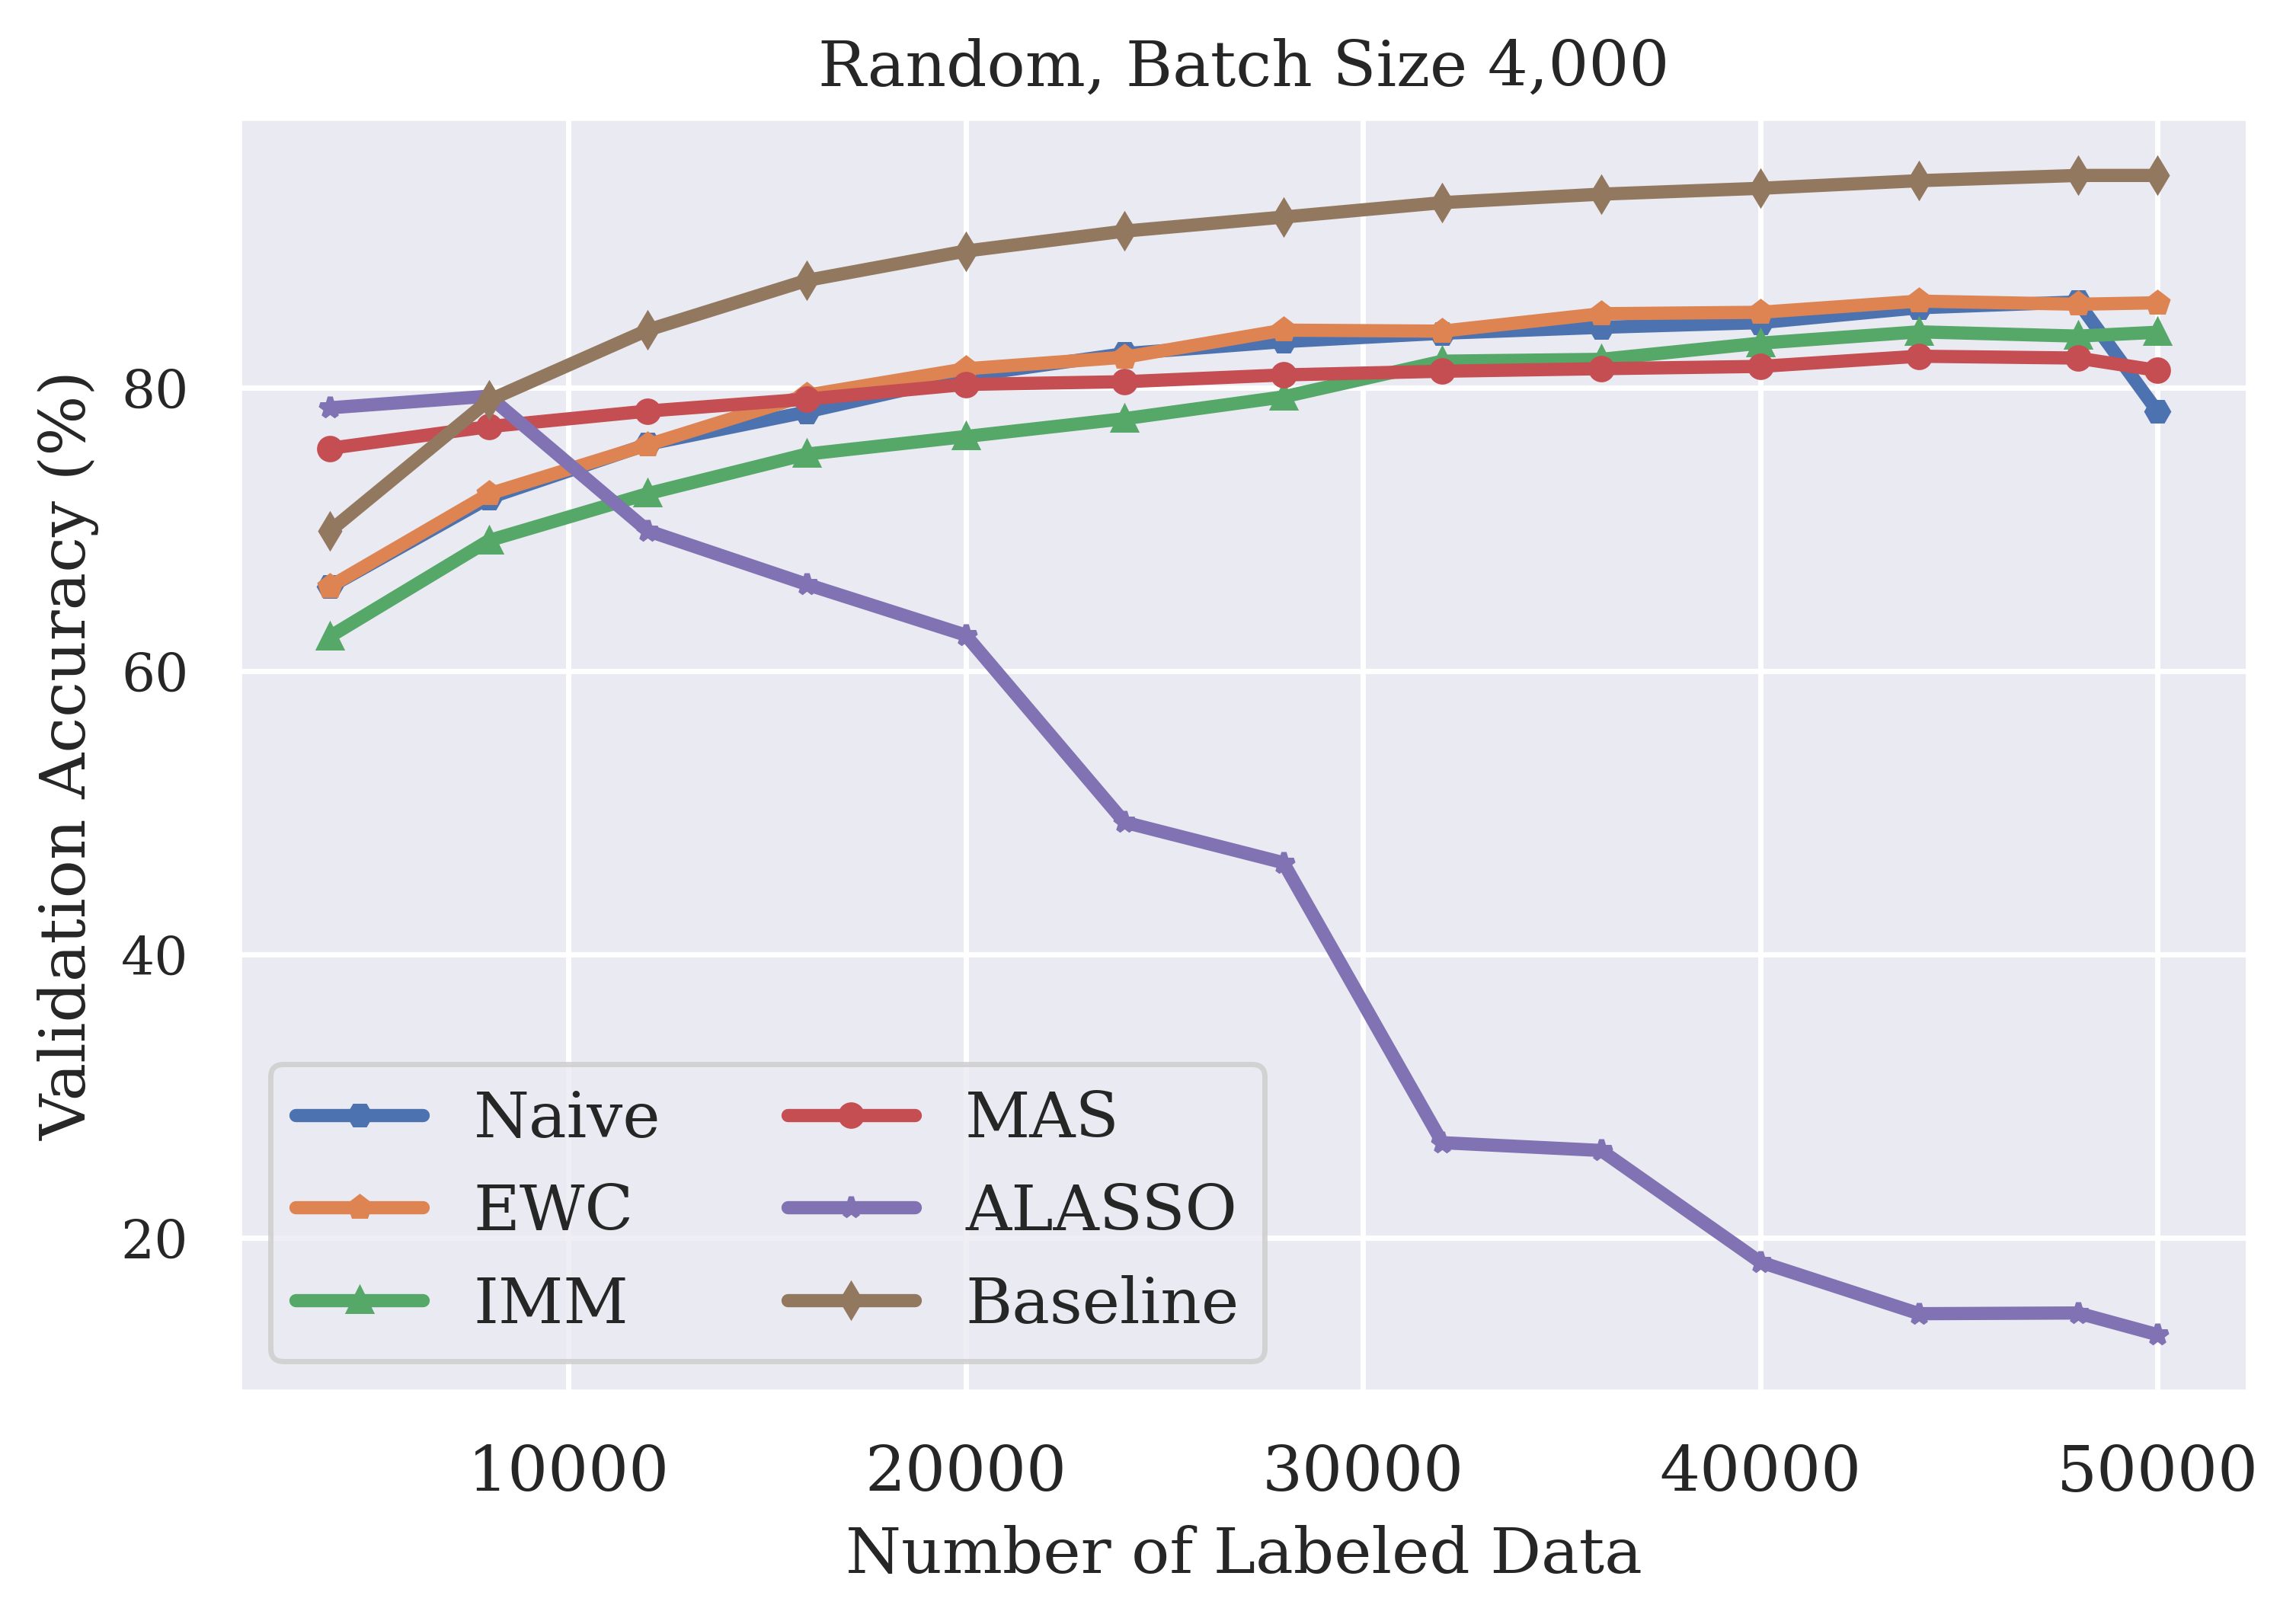
\includegraphics[width=0.32\linewidth]{images/results_CAL/random_4000b_acc.png} \hfill
    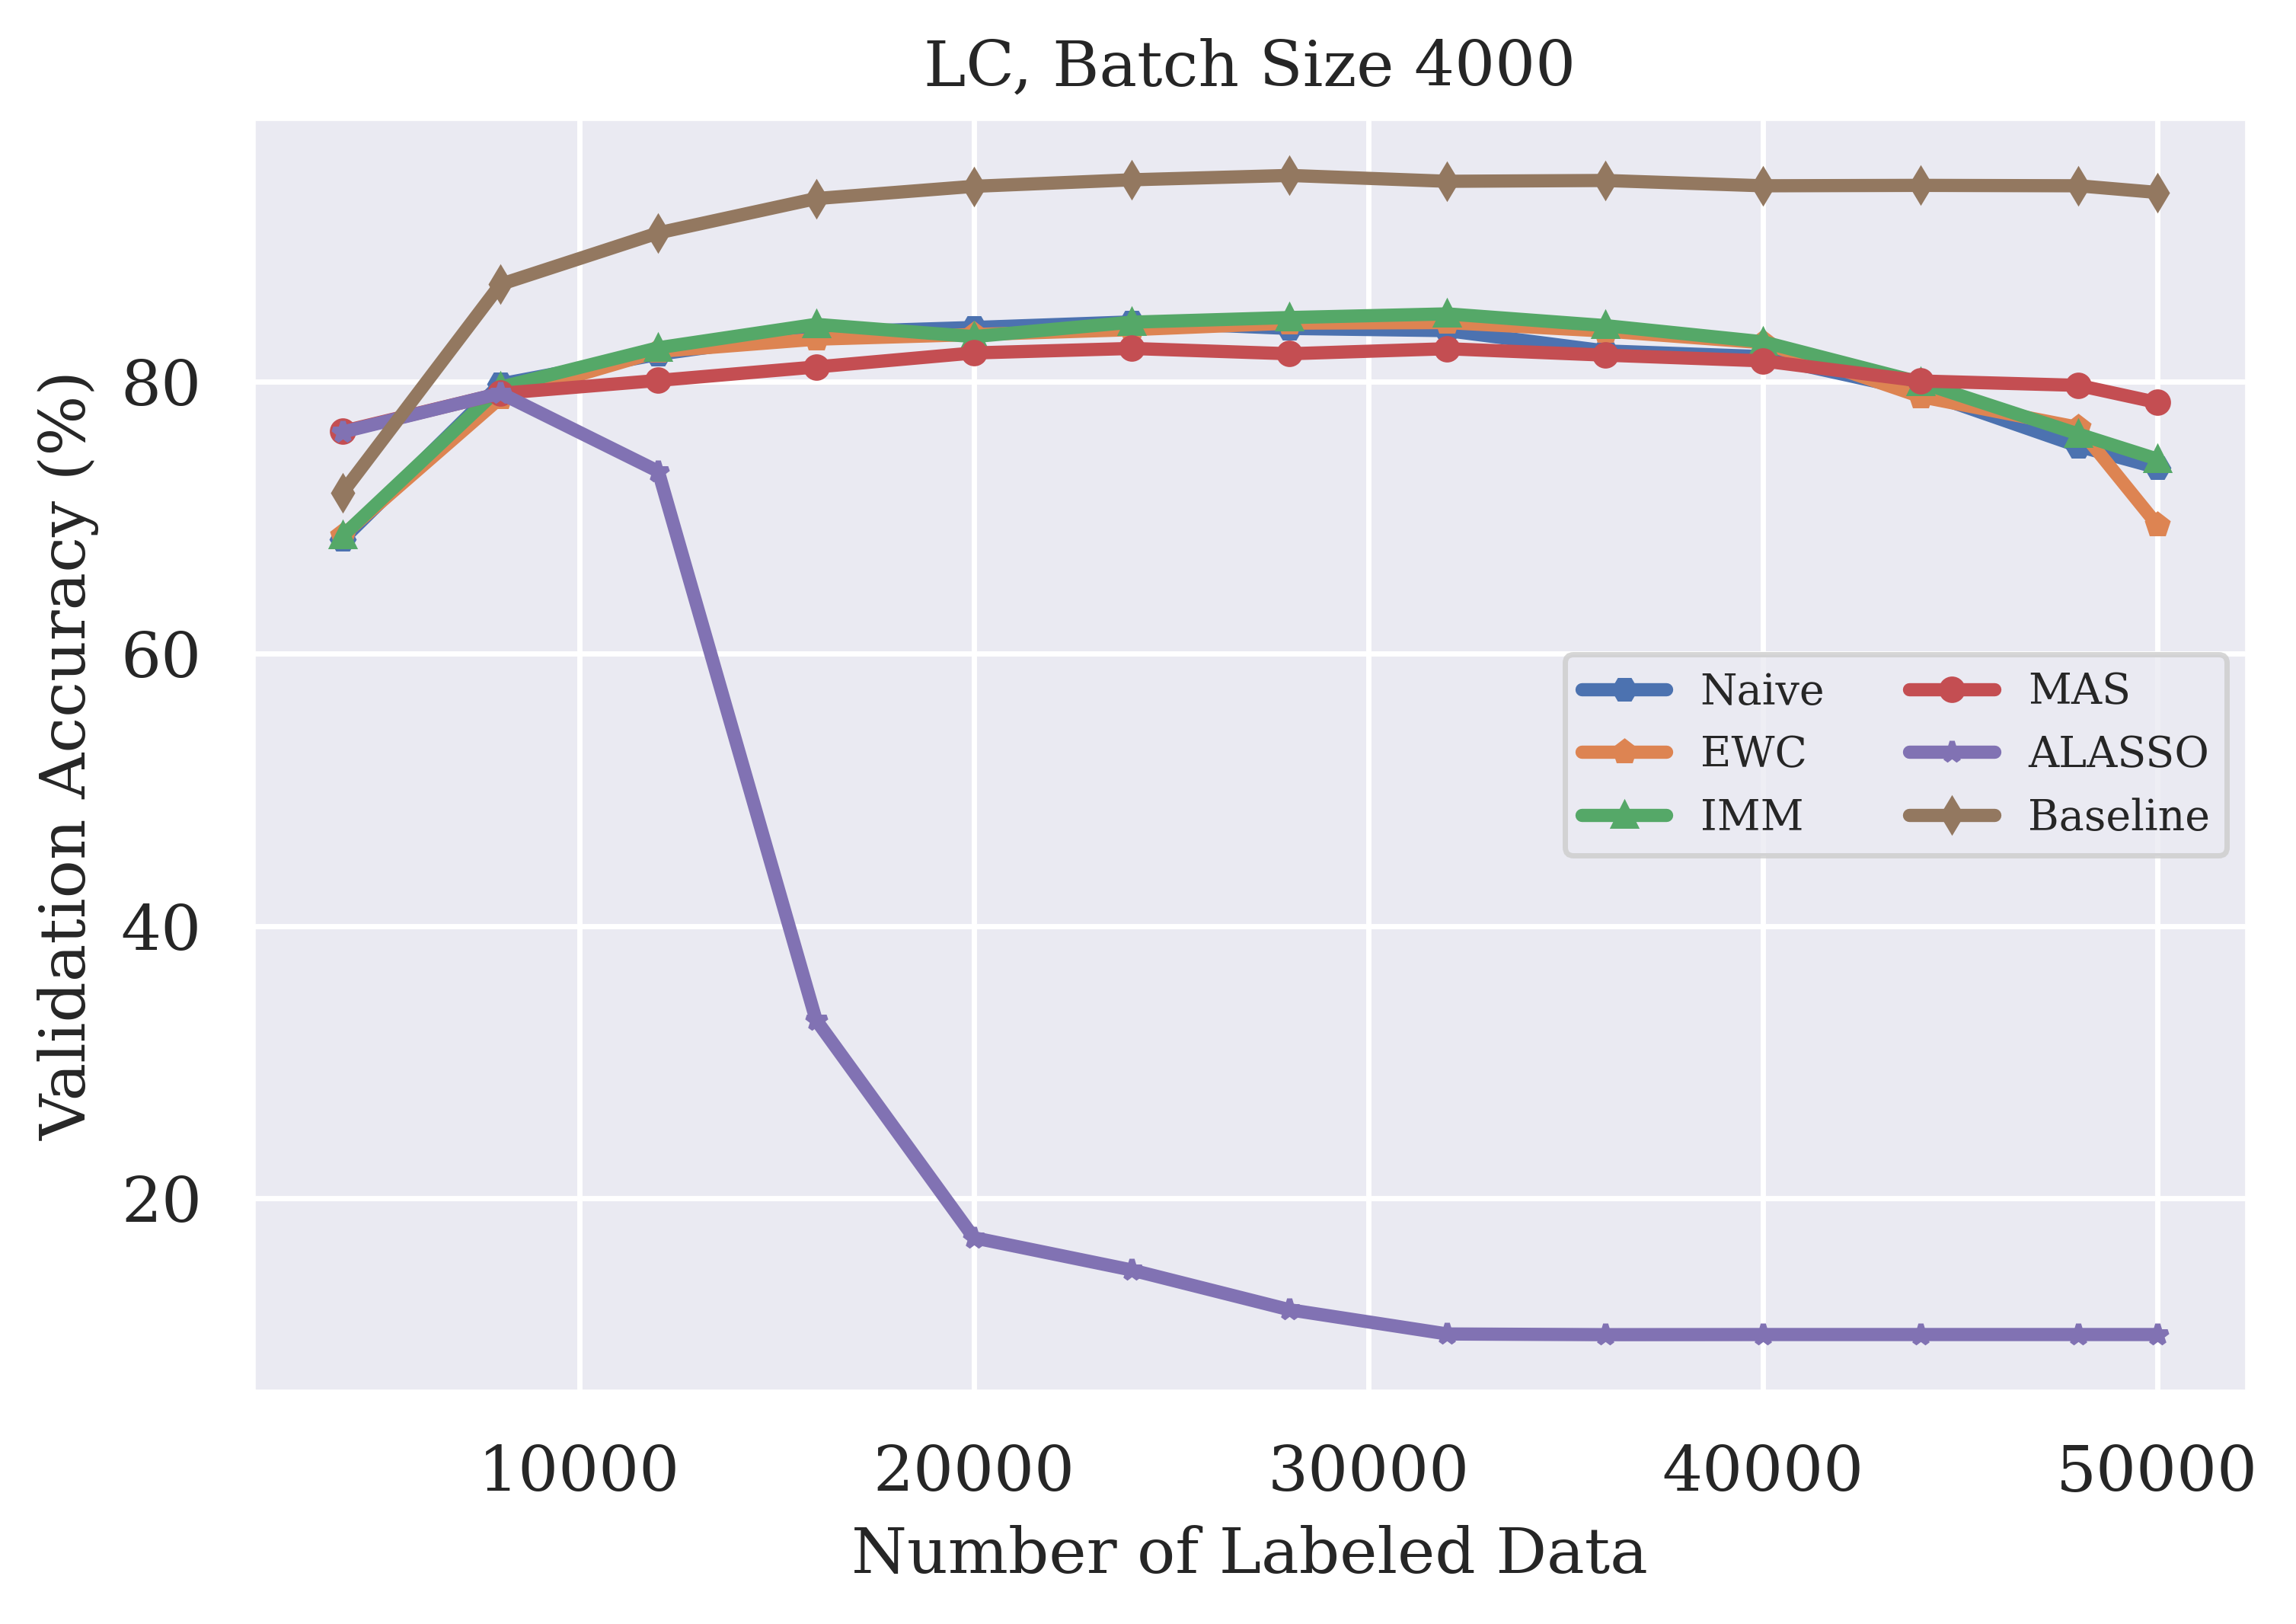
\includegraphics[width=0.32\linewidth]{images/results_CAL/lc_4000b_acc.png} \hfill
    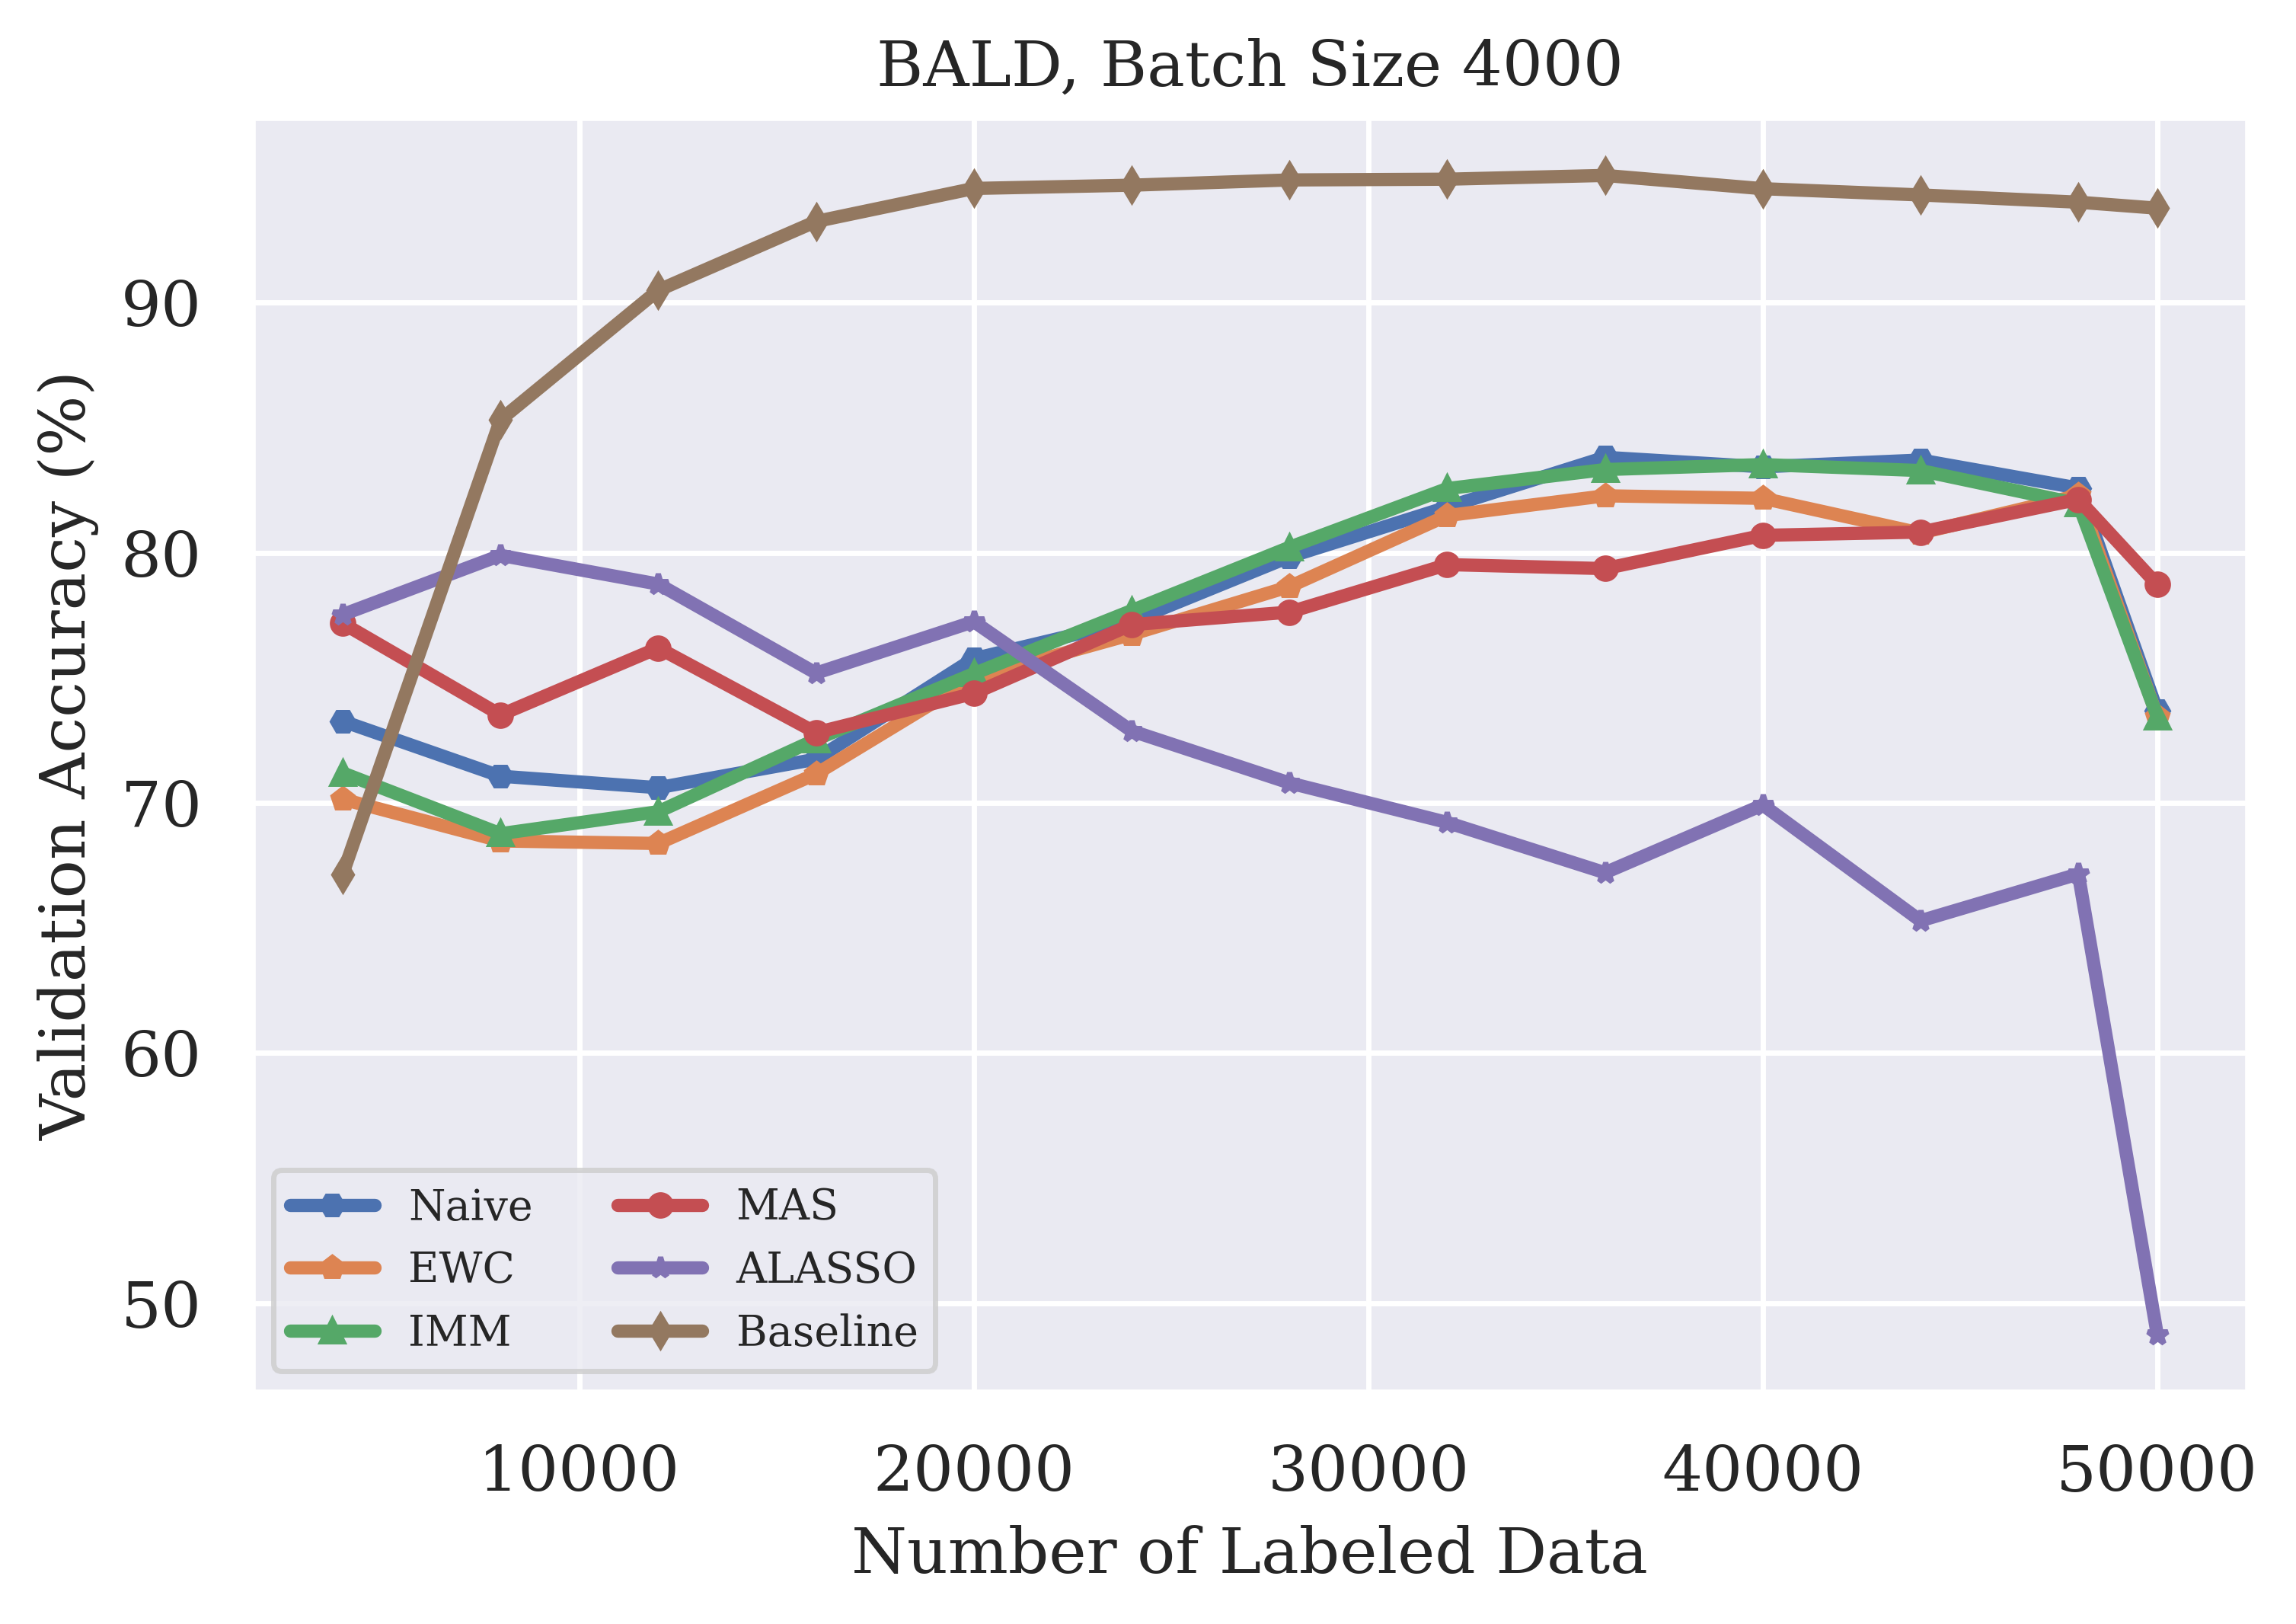
\includegraphics[width=0.32\linewidth]{images/results_CAL/bald_4000b_acc.png}
    \\[\smallskipamount]
    \hfill 
    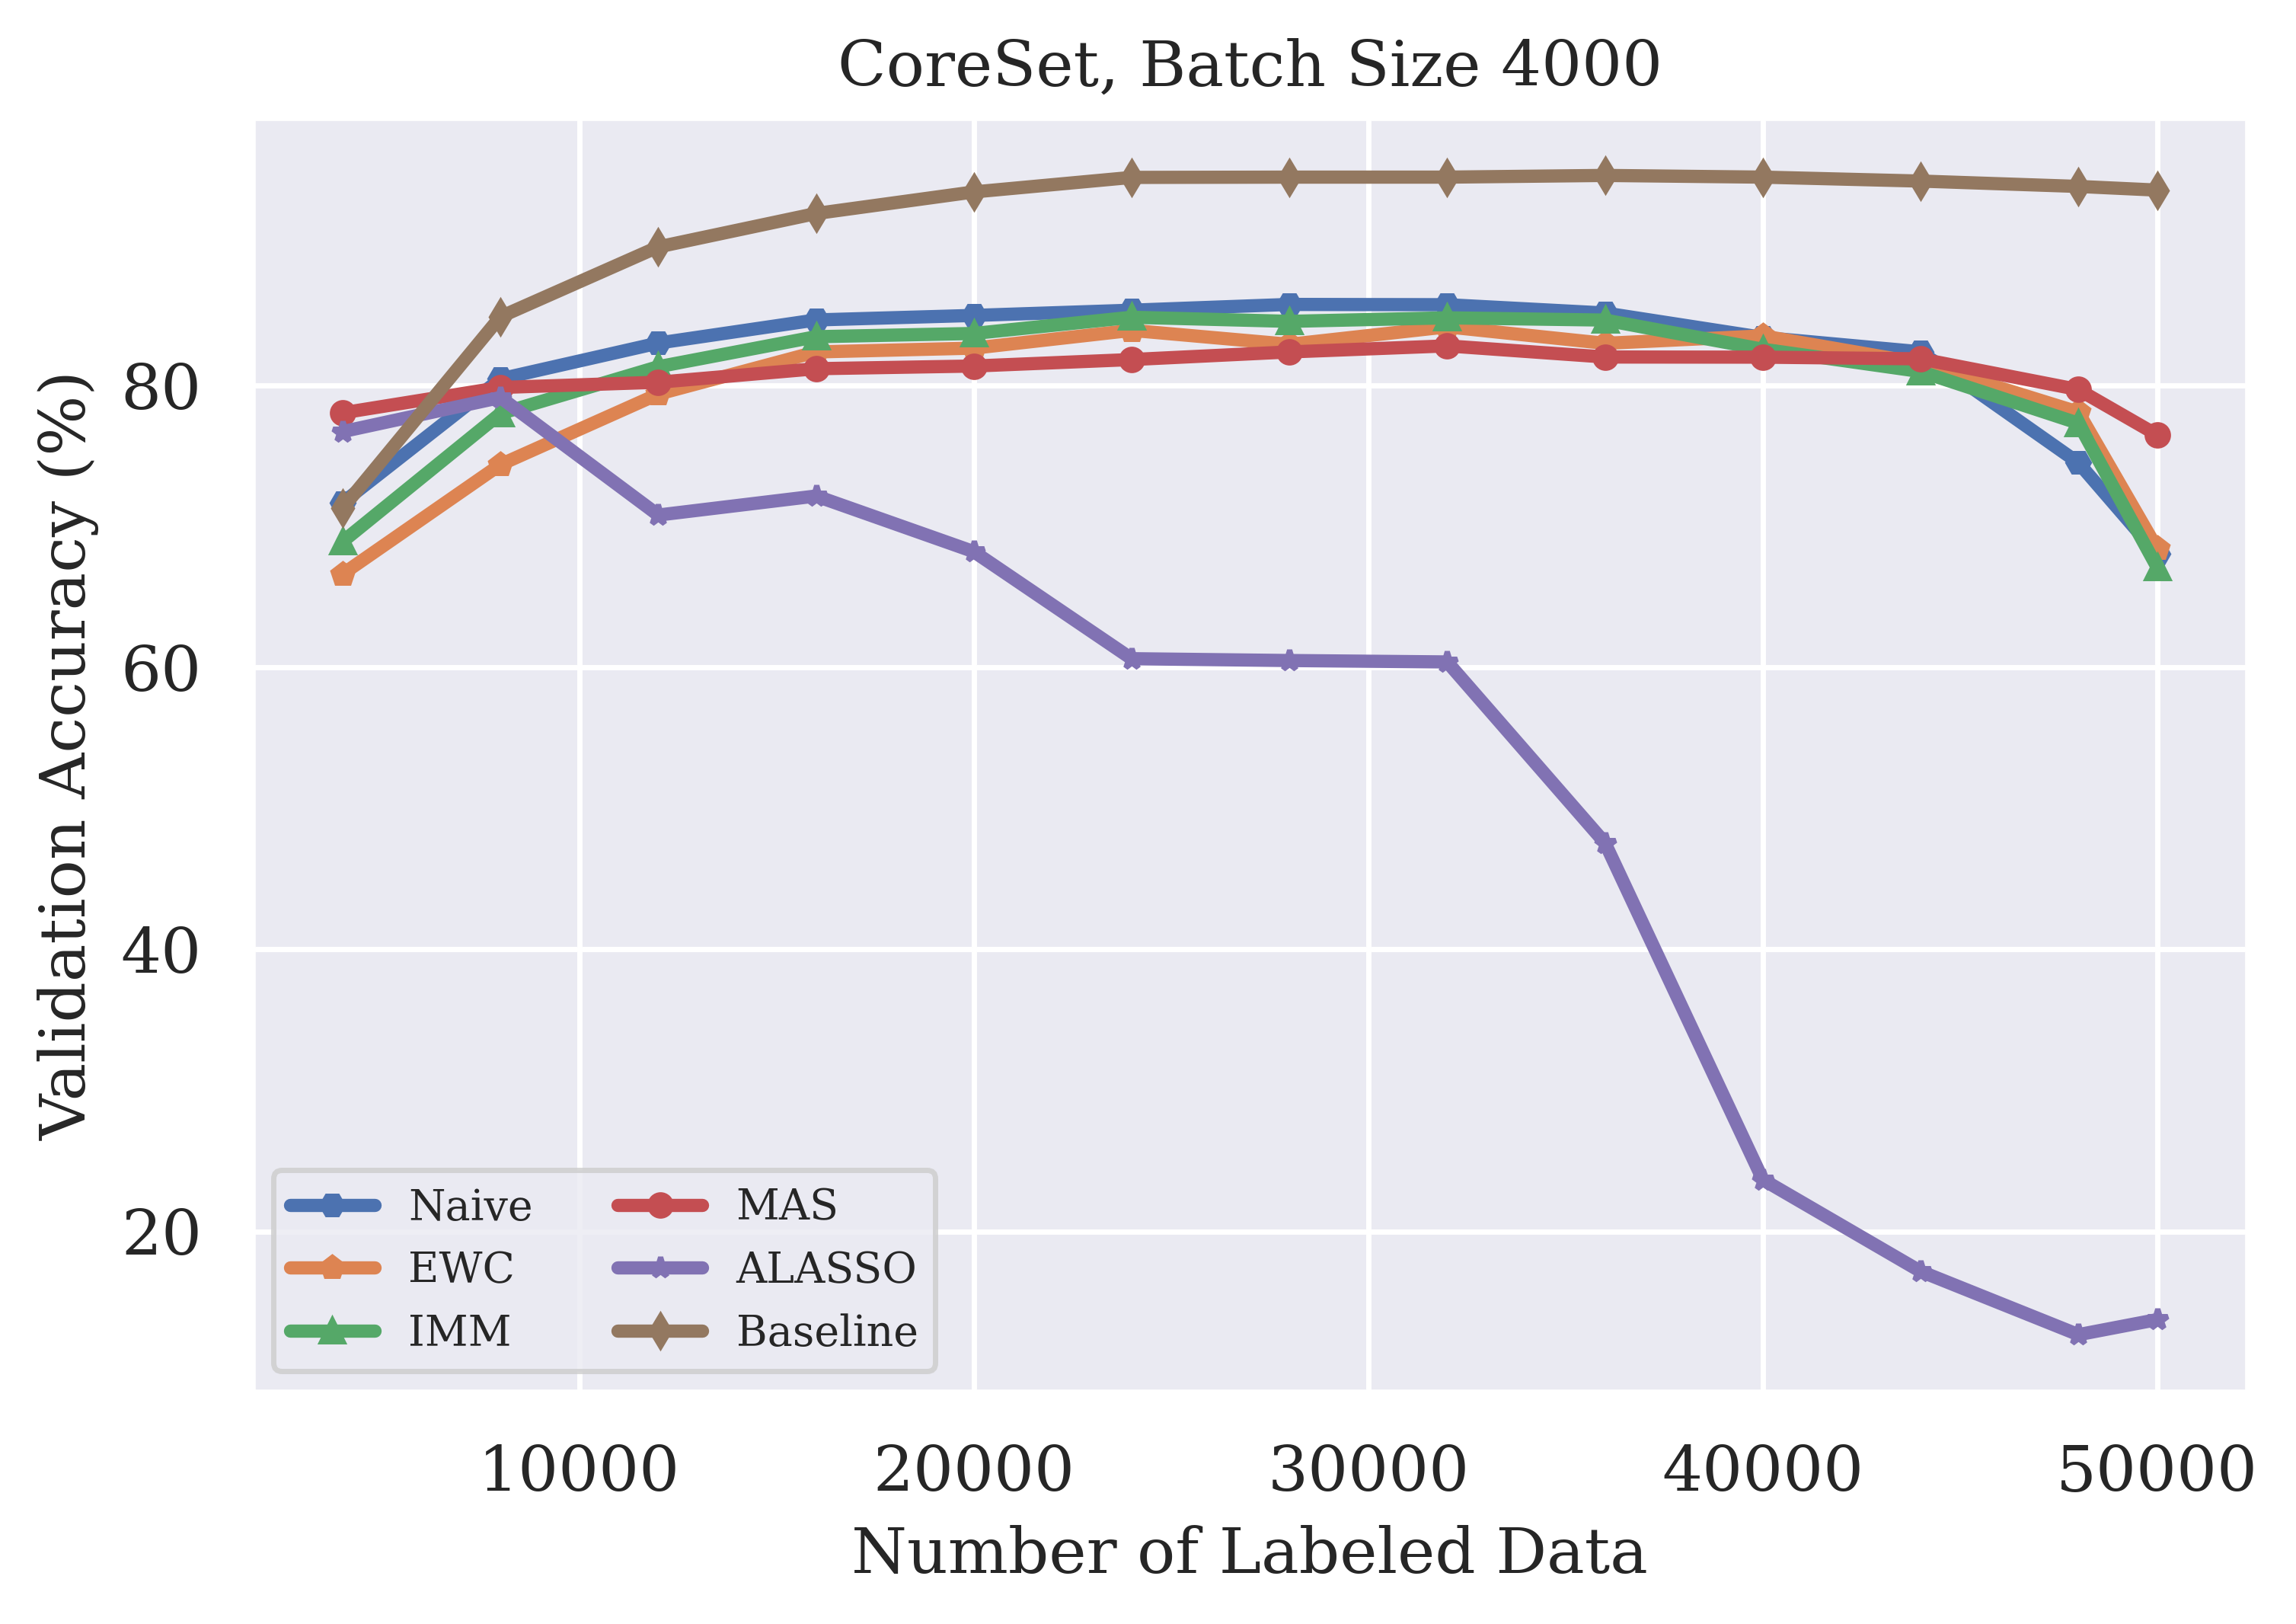
\includegraphics[width=0.32\linewidth]{images/results_CAL/coreset_4000b_acc.png} \hfill
    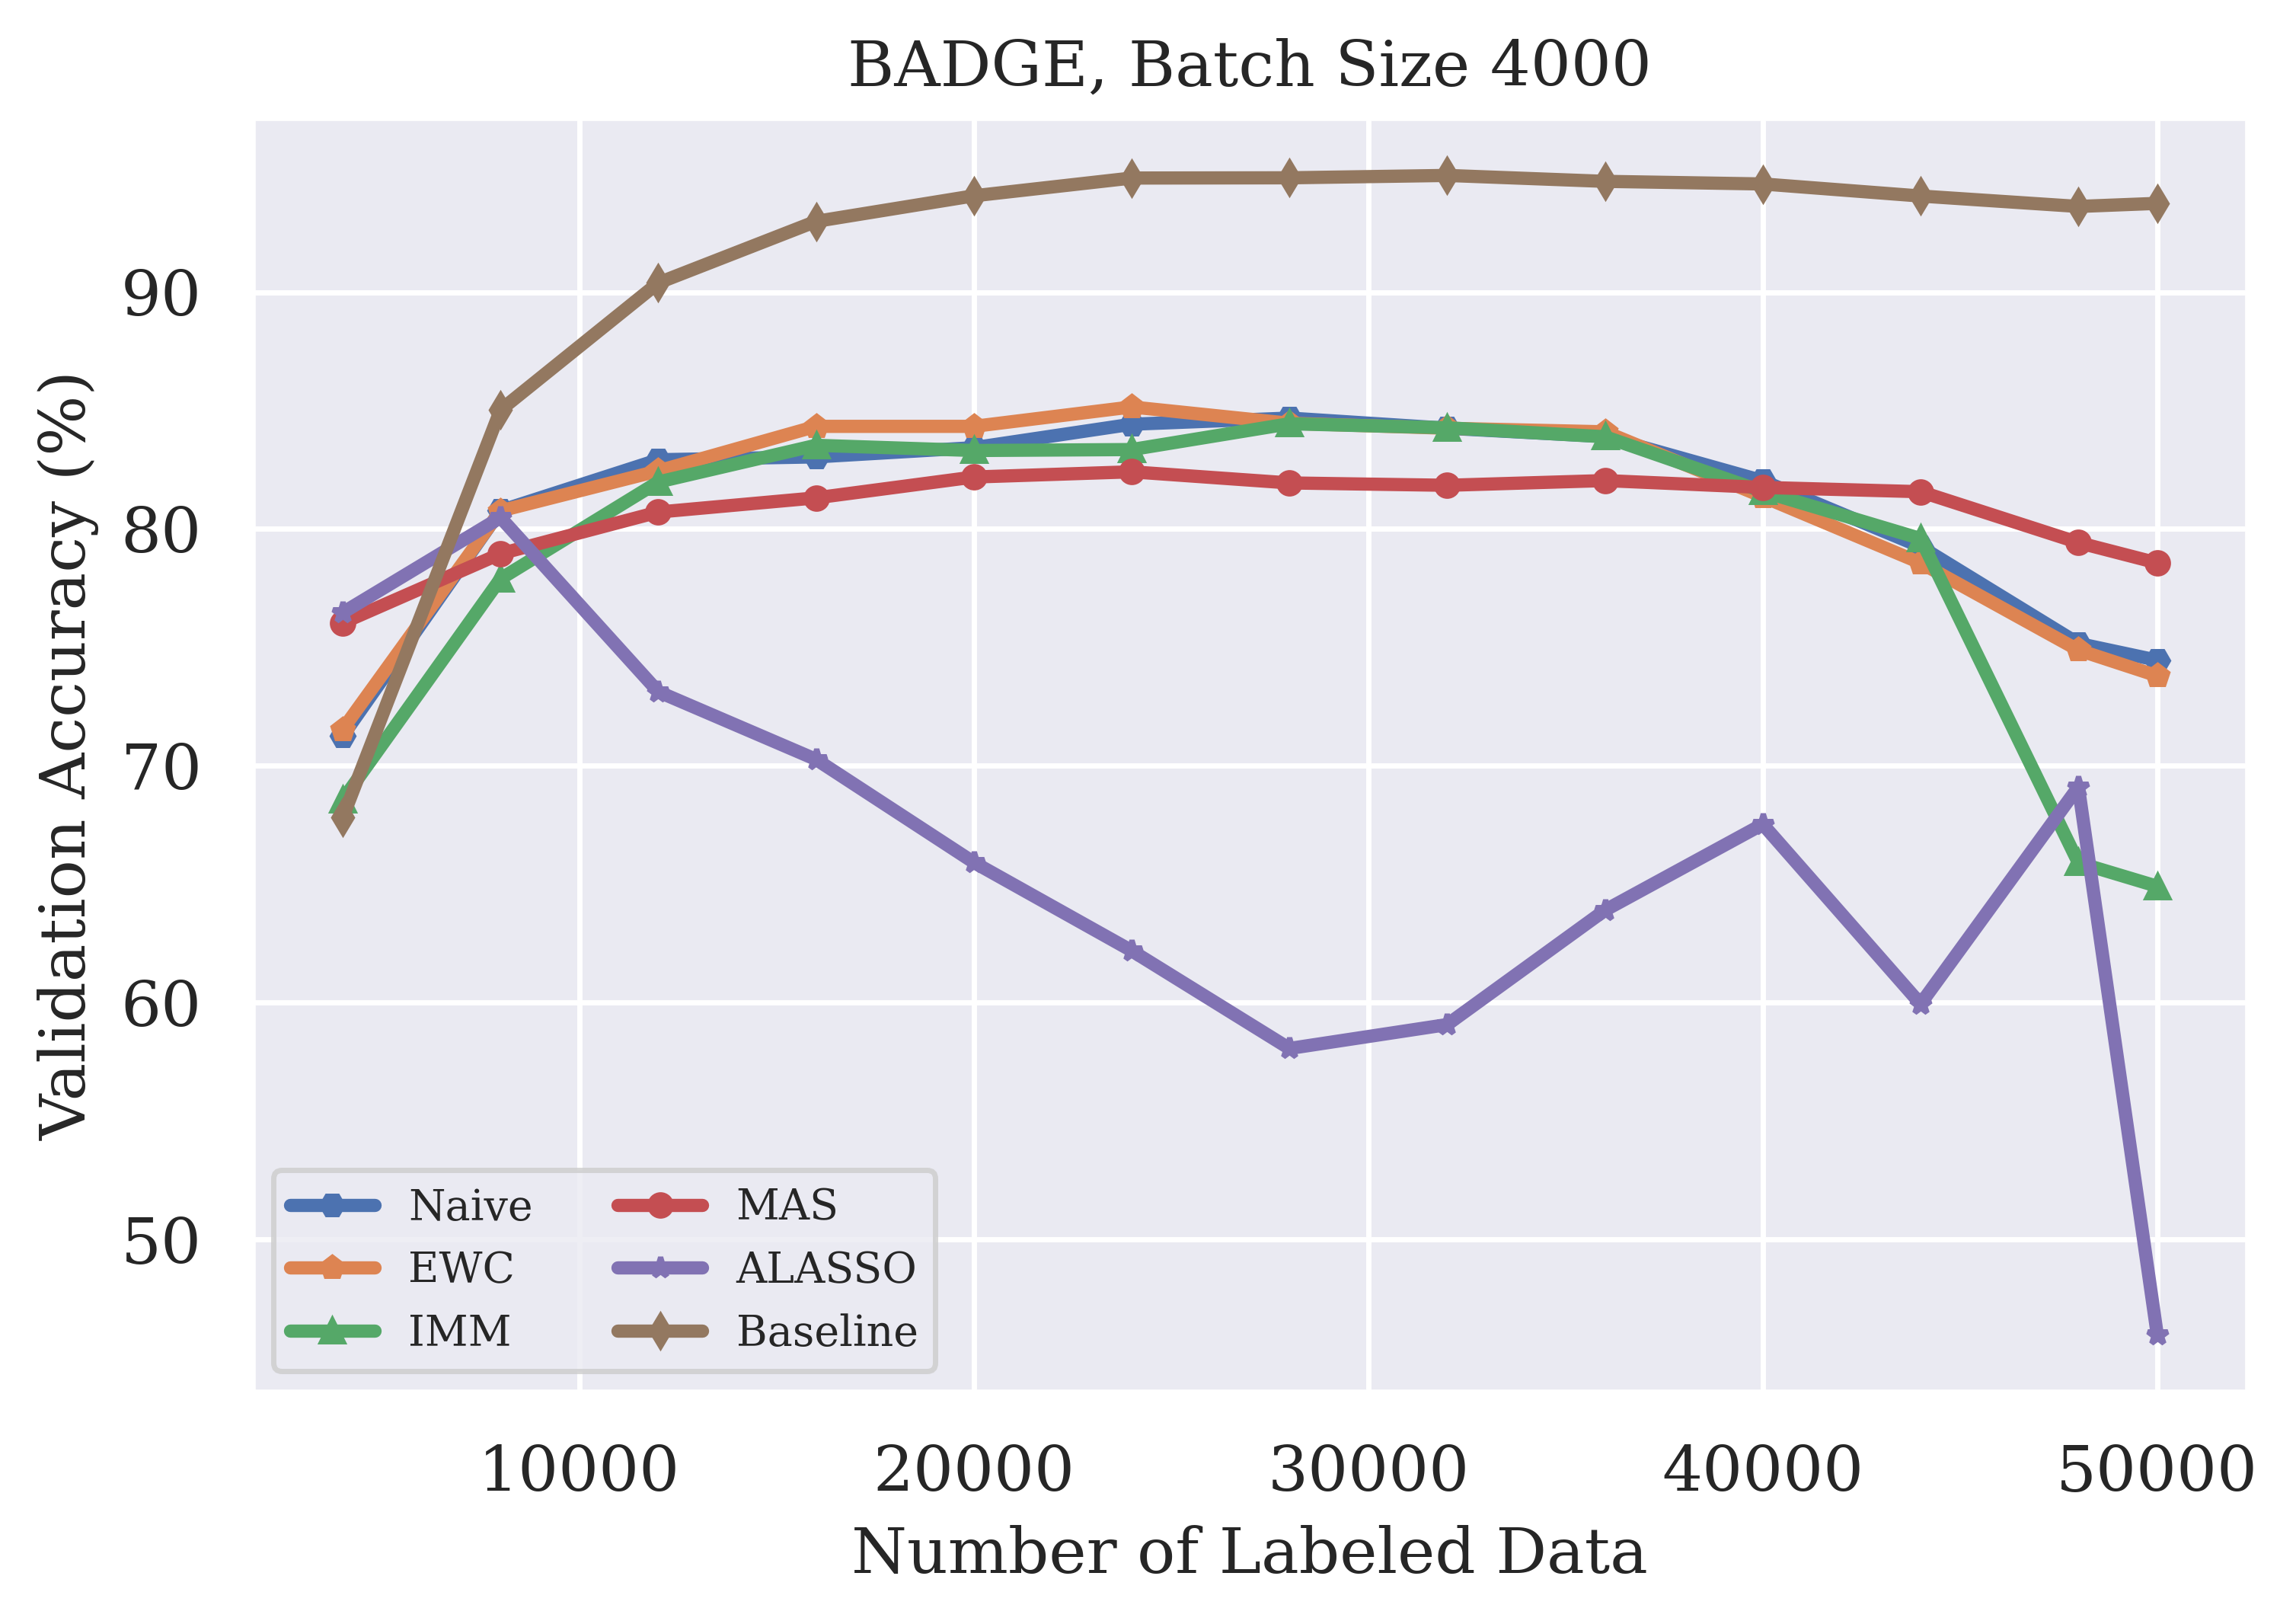
\includegraphics[width=0.32\linewidth]{images/results_CAL/badge_4000b_acc.png} \hfill
    \caption[Continual Active Learning with \gls{badge} with varying batch size]{Comparison of validation accuracy of regularization-based continual learning strategies
    with batch size 4000.}
    \label{fig:Evaluation:CAL:4000bAcc}
\end{figure}



\begin{table}[h]
    \centering
    \begin{tabular}{c | c c c c c } 
         & Random & \gls{lc} & \gls{bald} & CoreSet & \gls{badge}\\ 
        \hline
        Naive & 82 & 77 & 78 & 160 & 497 \\
        \gls{ewc} & 82 & 83 & 82 & 145 & 493\\
        \gls{imm} & 76 & 78 & 76 & 129 & 487\\
        \gls{mas} & 81 & 88 & 81 & 145 & 501\\
        \gls{alasso} & 118 & 127 & 120 & 189 & 534\\
        \hline 
        Baseline & 717 & 712 & 721 & 782 & 1311 \\
    \end{tabular}
    \caption{Comparison of execution time of regularization-based continual learning strategies
    with batch size 4000.}
    \label{fig:Evaluation:CAL:4000bTime}
\end{table}



\subsubsection{Influence of Batch Size}
\label{sec:Evaluation::CAL:ALRegCL:BatchSize}
Next, we study how the batch size of the selected active learning algorithm influences the results. To do so, we re-run each experiment from figure \ref{fig:Evaluation:CAL:4000bAcc}
with batch sizes 1,000 and 2,000. In this section, we only show the results for \gls{badge} since the results for the other active learning strategies are similar. For completeness, we
present the results of the remaining active learning strategies in appendix \ref{sec:Appendix:ContinualActiveLearning}. \par
In figure \ref{fig:Evaluation:Results:CAL:VaryBatchSizeAcc}, we present validation accuracy using \gls{badge} with batch sizes 1,000, 2,000, and 4,000. The execution times of these experiments
are displayed in table \ref{fig:Evaluation:CAL:BadgeVaryBatchSizeTime}, respectively. We notice a positive correlation between batch size and
validation accuracy. This correlation is caused by neural networks' tendency to overfit their training data. Since continual active learning methods only use the current batch as their training
samples in a given iteration, the neural network is more likely to overfit the training data. A commonly known remedy for this problem is increasing the amount of training data
\cite{ying2019overview}. Therefore, using a larger batch size yields better validation accuracy. Active learning algorithms, on the other hand, are not affected by overfitting because
they use the entire labeled pool for training. We can see that overfitting is an issue for small batch sizes not only because of the lower validation accuracy, but also because the validation
accuracy curve is more erratic. \par
In terms of execution time, we observe minor differences between the batch sizes for continual active learning and substantial differences for pure active learning. This is because the continual
active learning strategies will always use the same number of training data across a complete experiment, regardless of the batch size. Active learning methods, however, use the entire labeled pool
as their training data. In section \ref{sec:Methodology:CombiningCLandAL}, we mentioned that a model trained using active learning with a total budget of $n$ and a batch size of $b$ is trained
on $\frac{n(n+b)}{2b}$ samples. To demonstrate the influence of the batch size in this setting, we calculate the total number of samples trained. The results are given in table 
\ref{fig:NumberOfTrainingPoints}. We can see that the number of training samples behaves anti-proportionally to the batch size. Therefore, the total execution time is higher for smaller batch sizes.
Note, however, that this behavior is not anti-proportional, because the total execution time is broken down into training and query time. The training time is anti-proportional
to the batch size. The query time, however, remains constant because the batch size does not influence the total amount of queried points. \par

\begin{figure}[h]
    \centering
    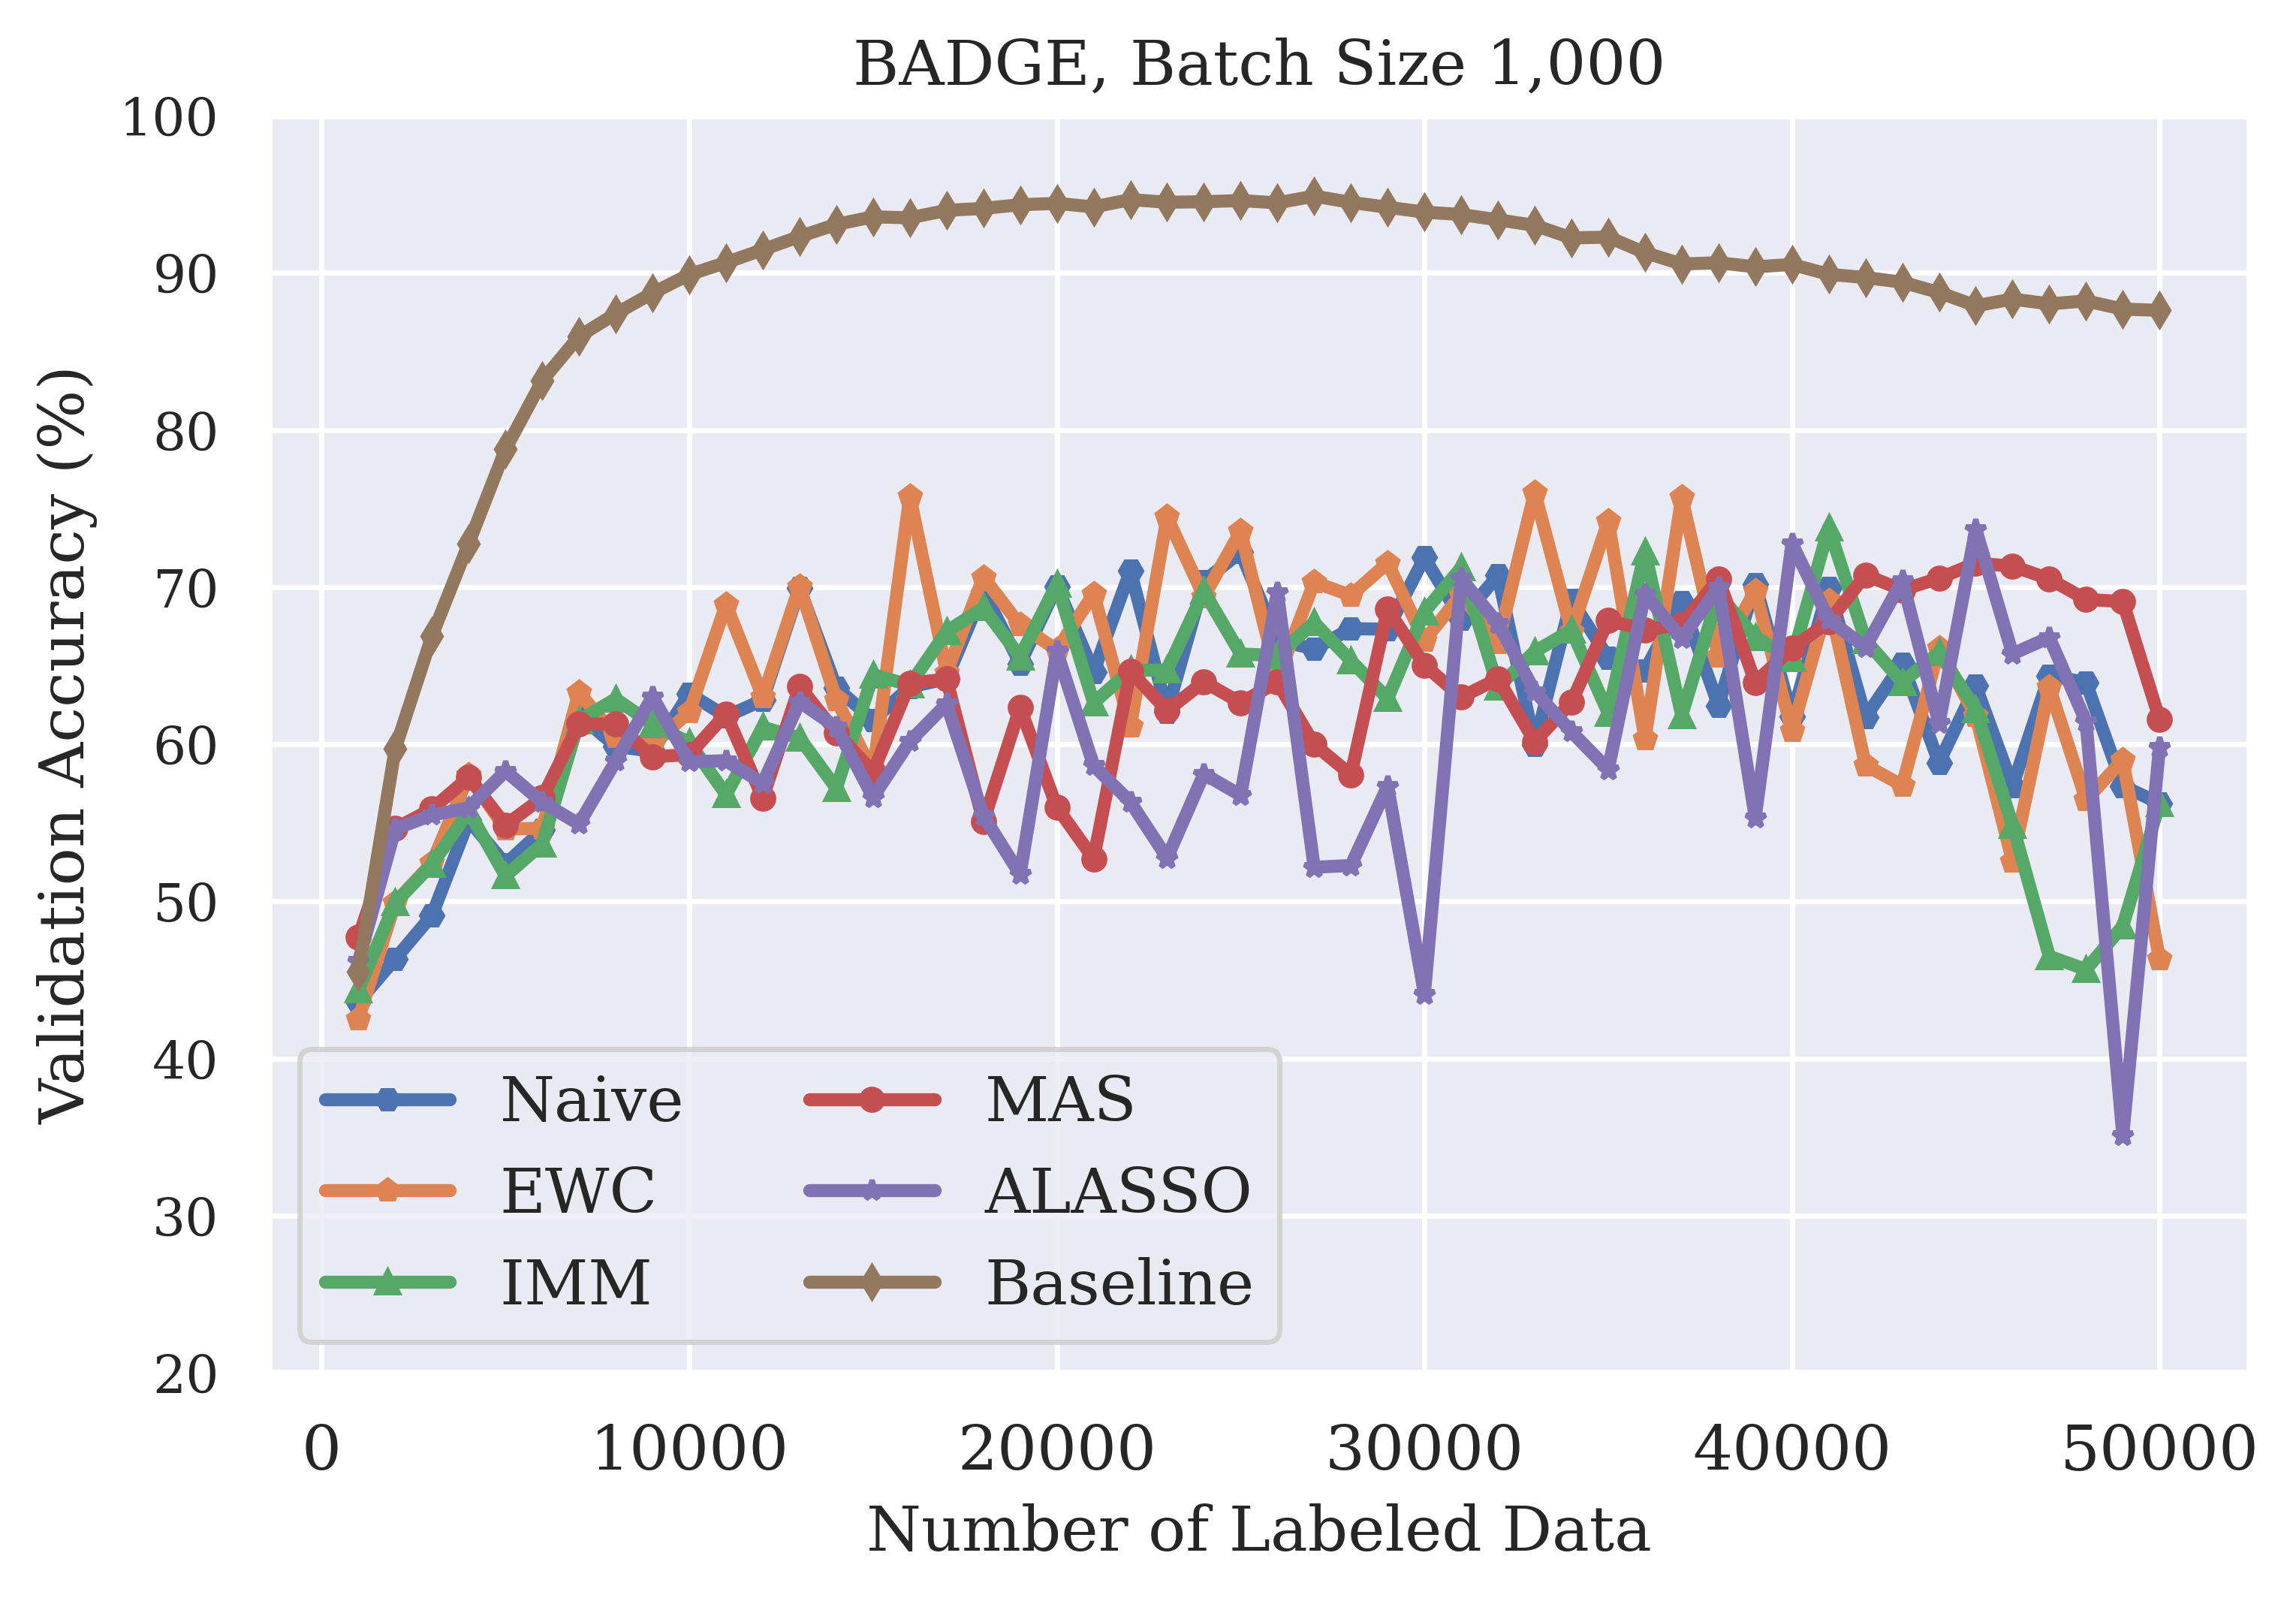
\includegraphics[width=0.32\linewidth]{images/results_CAL/badge_1000b_Comp.png} \hfill
    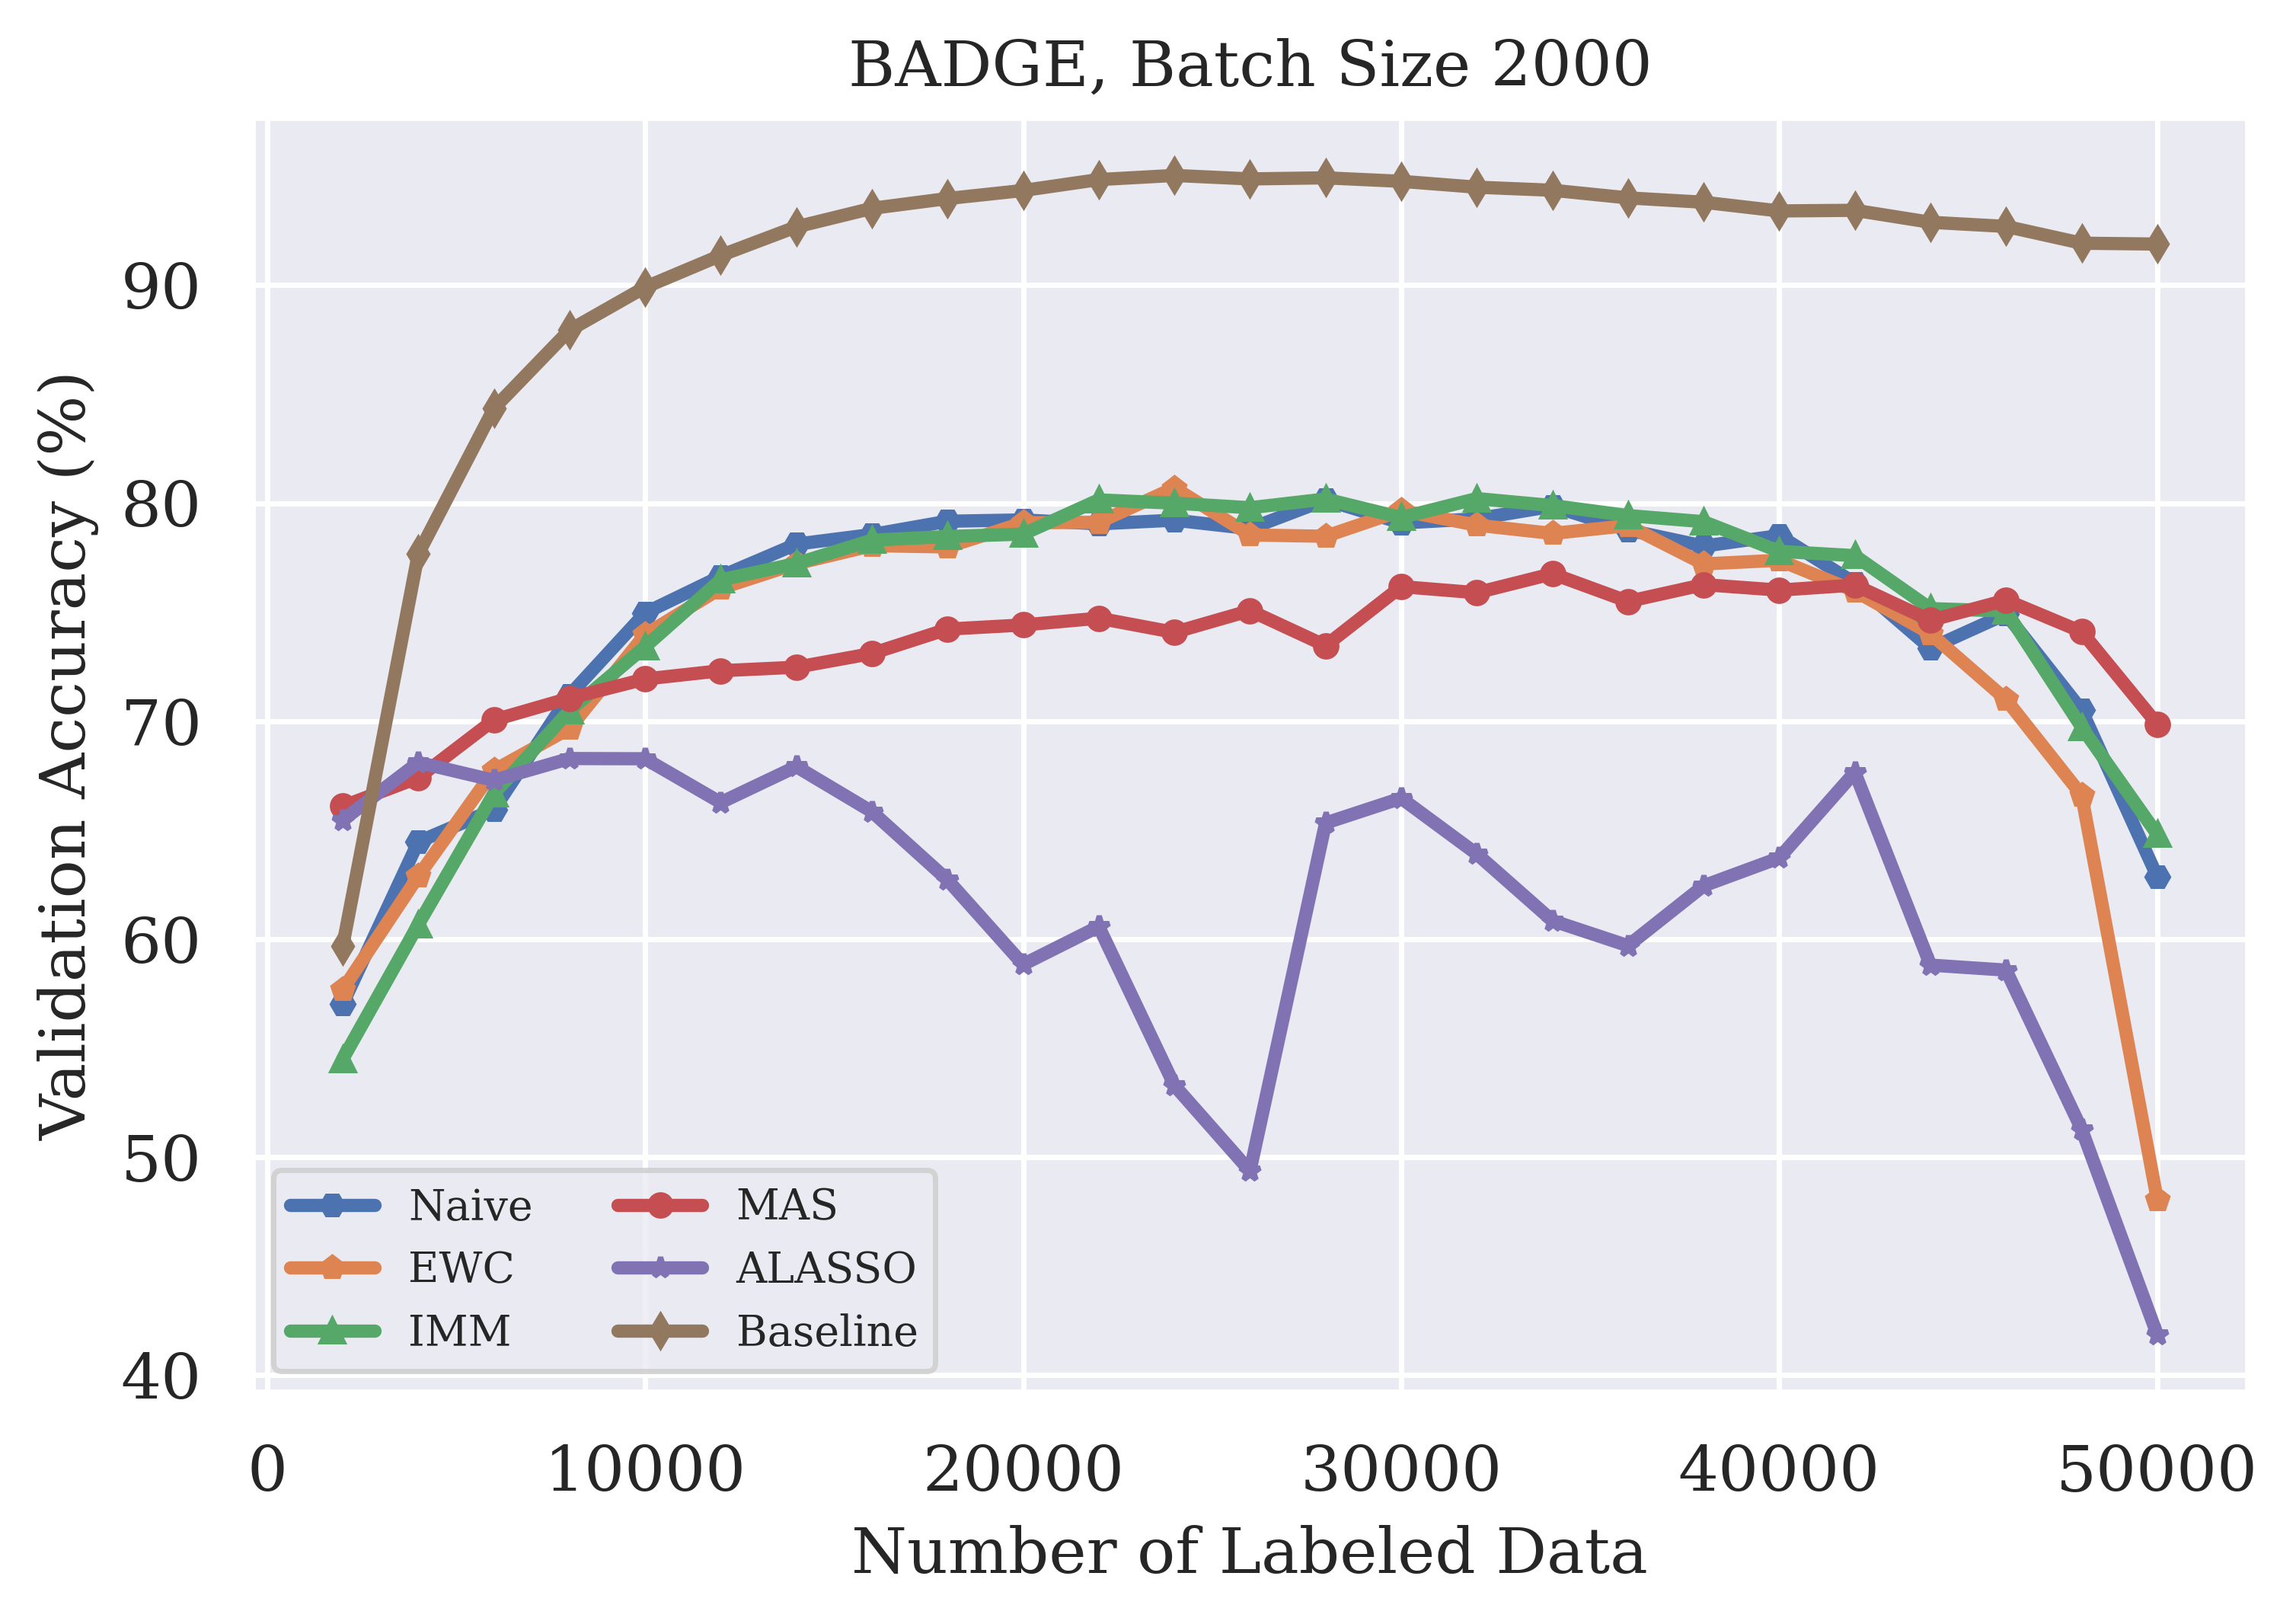
\includegraphics[width=0.32\linewidth]{images/results_CAL/badge_2000b_acc.png} \hfill
    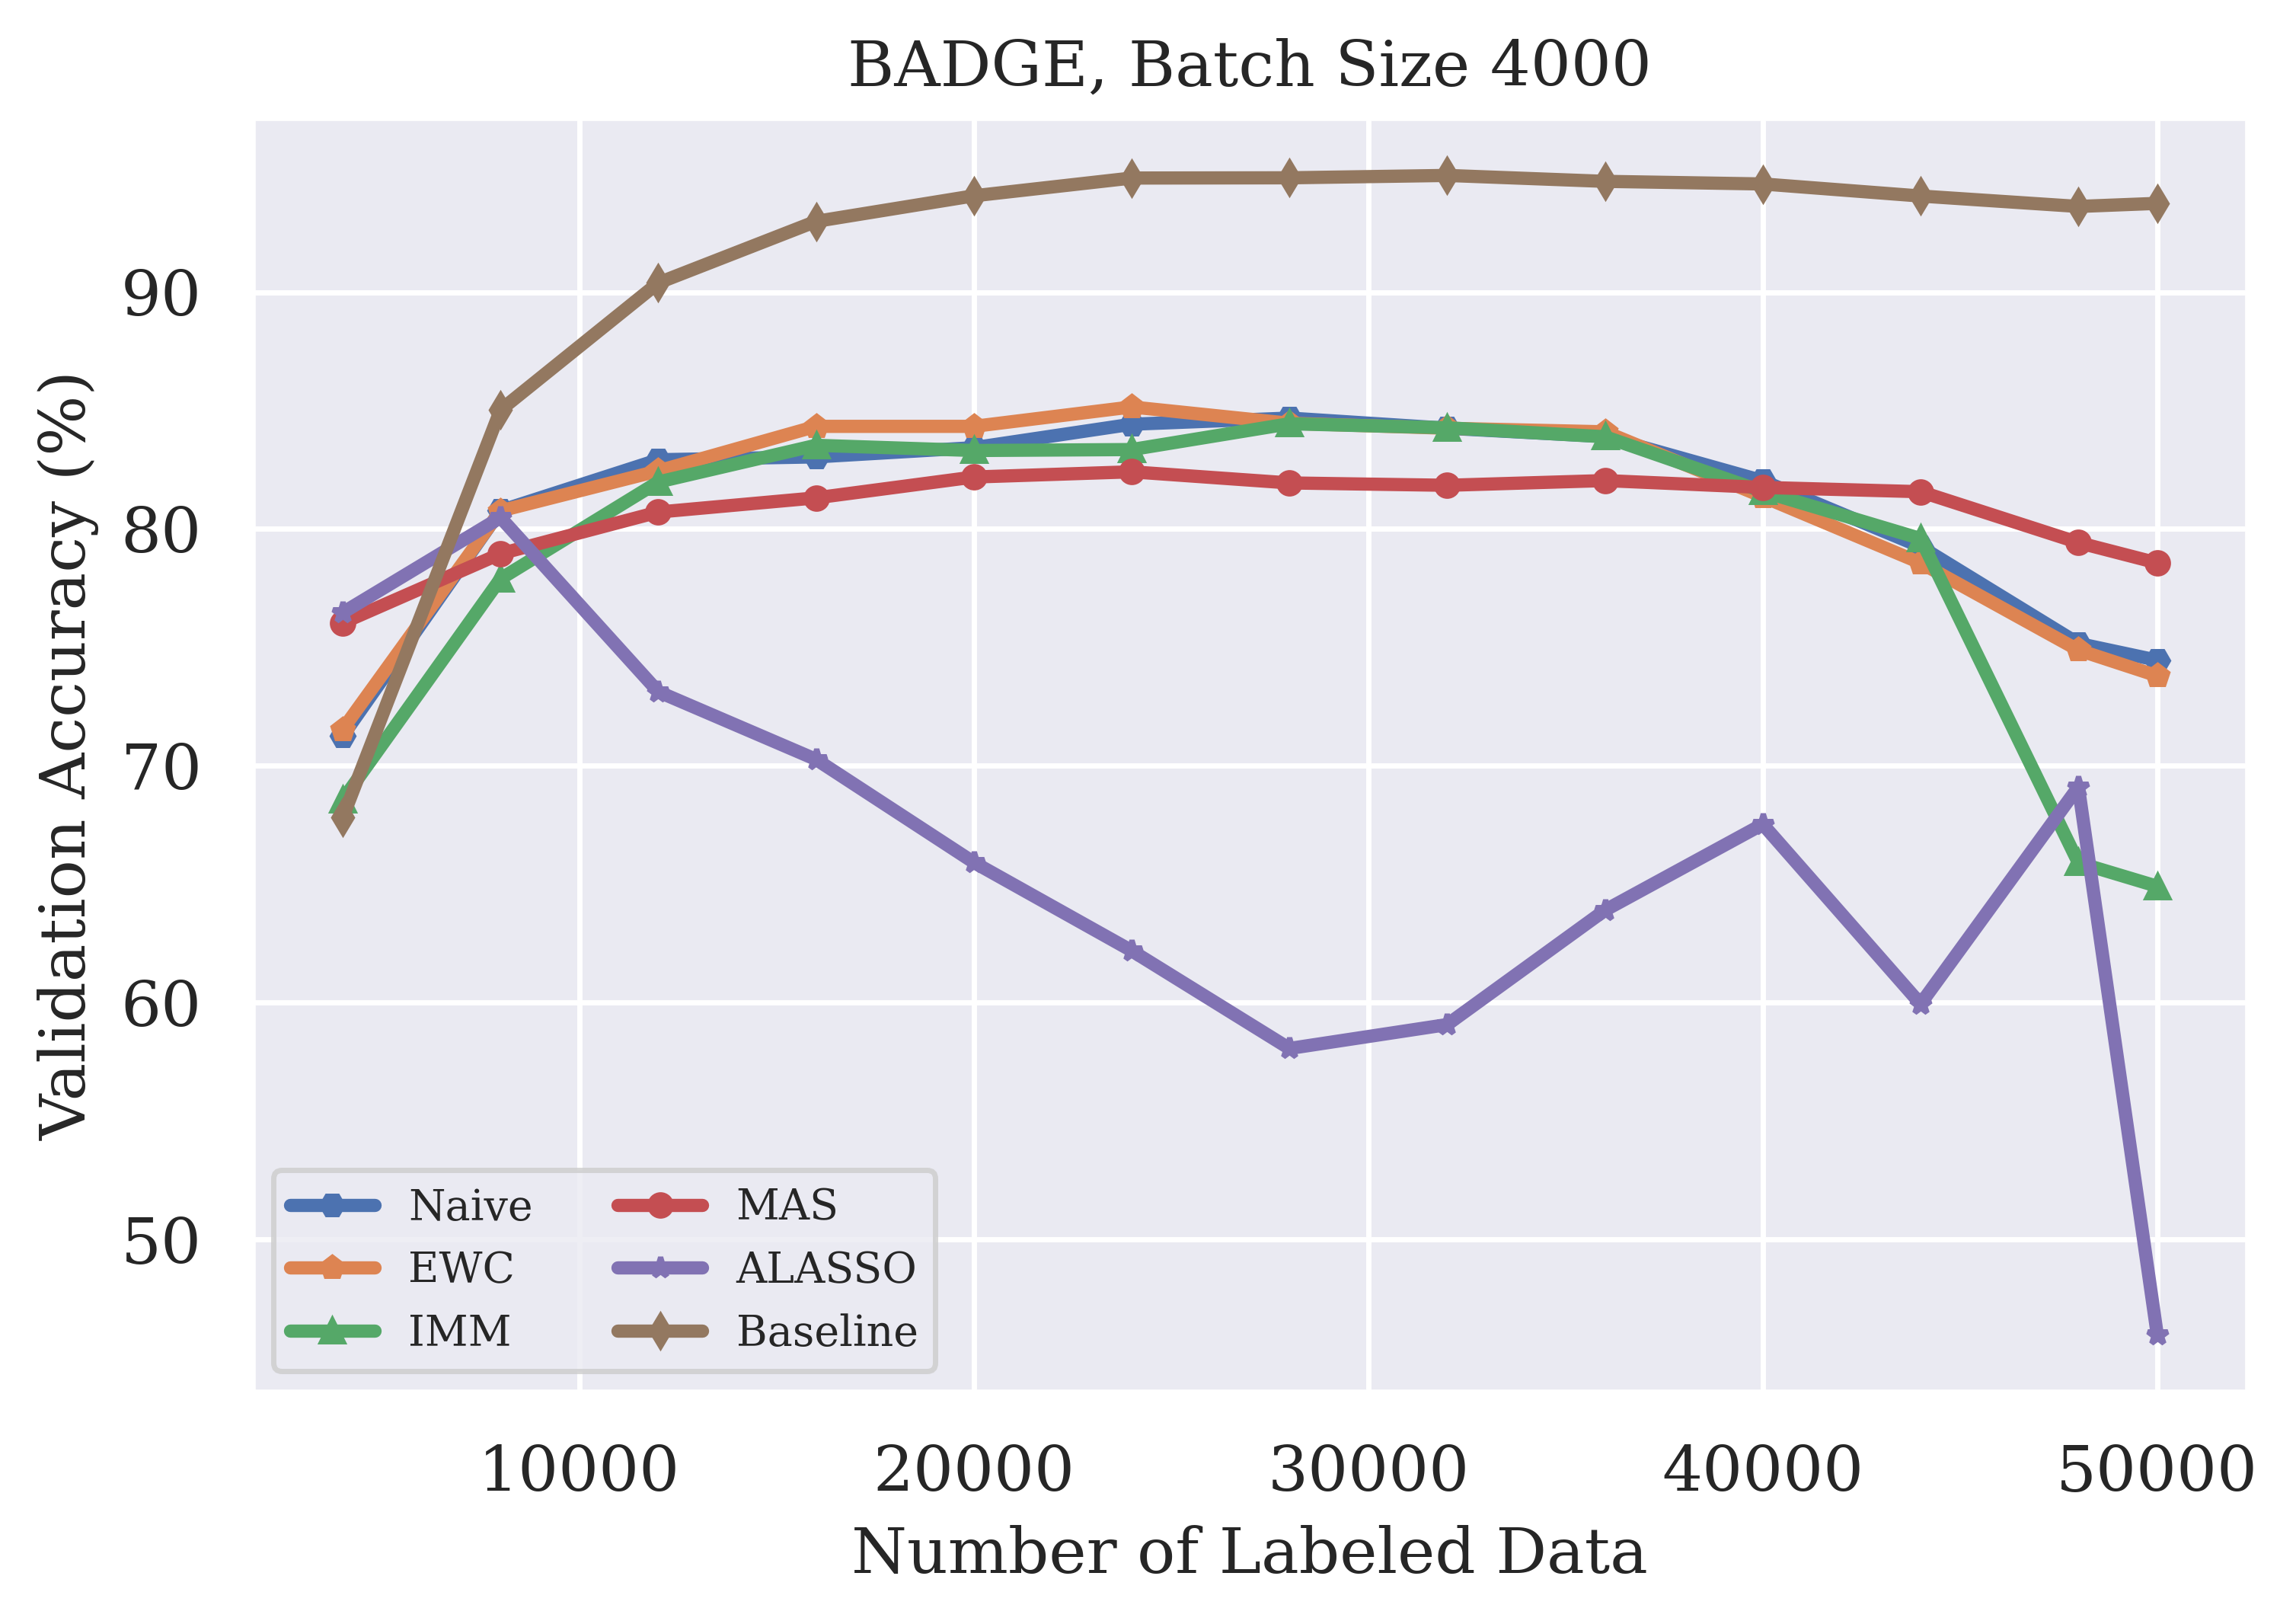
\includegraphics[width=0.32\linewidth]{images/results_CAL/badge_4000b_acc.png}
    \caption[Continual Active Learning with \gls{badge} with varying batch size]{Comparison of validation accuracy of Continual Learning strategies used with the Active Learning strategy
    \gls{badge}.}
    \label{fig:Evaluation:CAL:VaryBatchSizeAcc}
\end{figure}


\begin{table}[h]
    \centering
    \begin{tabular}{c | c c c c c c} 
        Batch Size & Baseline & Naive & \gls{ewc} & \gls{imm} & \gls{mas} & \gls{alasso}\\ 
        \hline 
        4000 & 1311 & 497 & 493 & 487 & 501 & 534 \\
        2000 & 1935 & 523 & 513 & 500 & 515 & 547 \\
        1000 & 3171 & 493 & 486 & 501 & 505 & 509 \\
    \end{tabular}
    \caption{Comparison of execution time of regularization-based continual learning strategies
    combined with \gls{badge}.}
    \label{fig:Evaluation:CAL:BadgeVaryBatchSizeTime}
\end{table}

\begin{table}[h]
    \centering
    \begin{tabular}{c | c } 
        $b$ & Total number of training points \\
        \hline 
        1000 & 1275000 \\
        2000 & 650000 \\
        4000 & 362000 \\
    \end{tabular}
    \caption{Total number of training points for varying batch sizes on the CIFAR-10 dataset}
    \label{fig:Evaluation:CAL:NumberOfTrainingPoints}
\end{table}


\subsubsection{Delaying the Start of Continual Learning}
\label{sec:Evaluation:CAL:ALRegCL:Hybrid}
After running the experiments in figure \ref{fig:Evaluation:CAL:4000bAcc}, we notice that all of them demonstrate a significant discrepancy in validation accuracy
between active learning and continual active learning. To further investigate this gap, we evaluate a hybrid approach where we run active learning for the first $i$
iterations before switching to continual active learning. With these experiments, we hope to decrease the gap in validation accuracy to active learning. We vary $i$
between 0 and 6, and perform two sets of experiments, one using the continual learning strategy \gls{mas} and the other using \gls{ewc}. In both experiments, we use
the active learning strategy \gls{badge}. The results of the two sets of experiments can be found in figure  \ref{fig:Evaluation:Results:CAL:DelayedStart}. For \gls{mas}
and \gls{ewc}, the validation accuracy drops immediately after switching from active learning to continual active learning. However, in the long run \gls{mas}
retains validation accuracy better than \gls{ewc}. We also notice that while the validation accuracy does drop after switching to continual active learning, the accuracy
progression after the switch outperforms continual active learning. We attribute these two observations to the regularization effect of \gls{mas} and \gls{ewc}. 
The reason why \gls{mas} performs better than \gls{ewc} in this setting is because it employs heavier regularization than \gls{ewc}, which we observed in previous
experiments. \par

\begin{figure}[h]
    \centering
    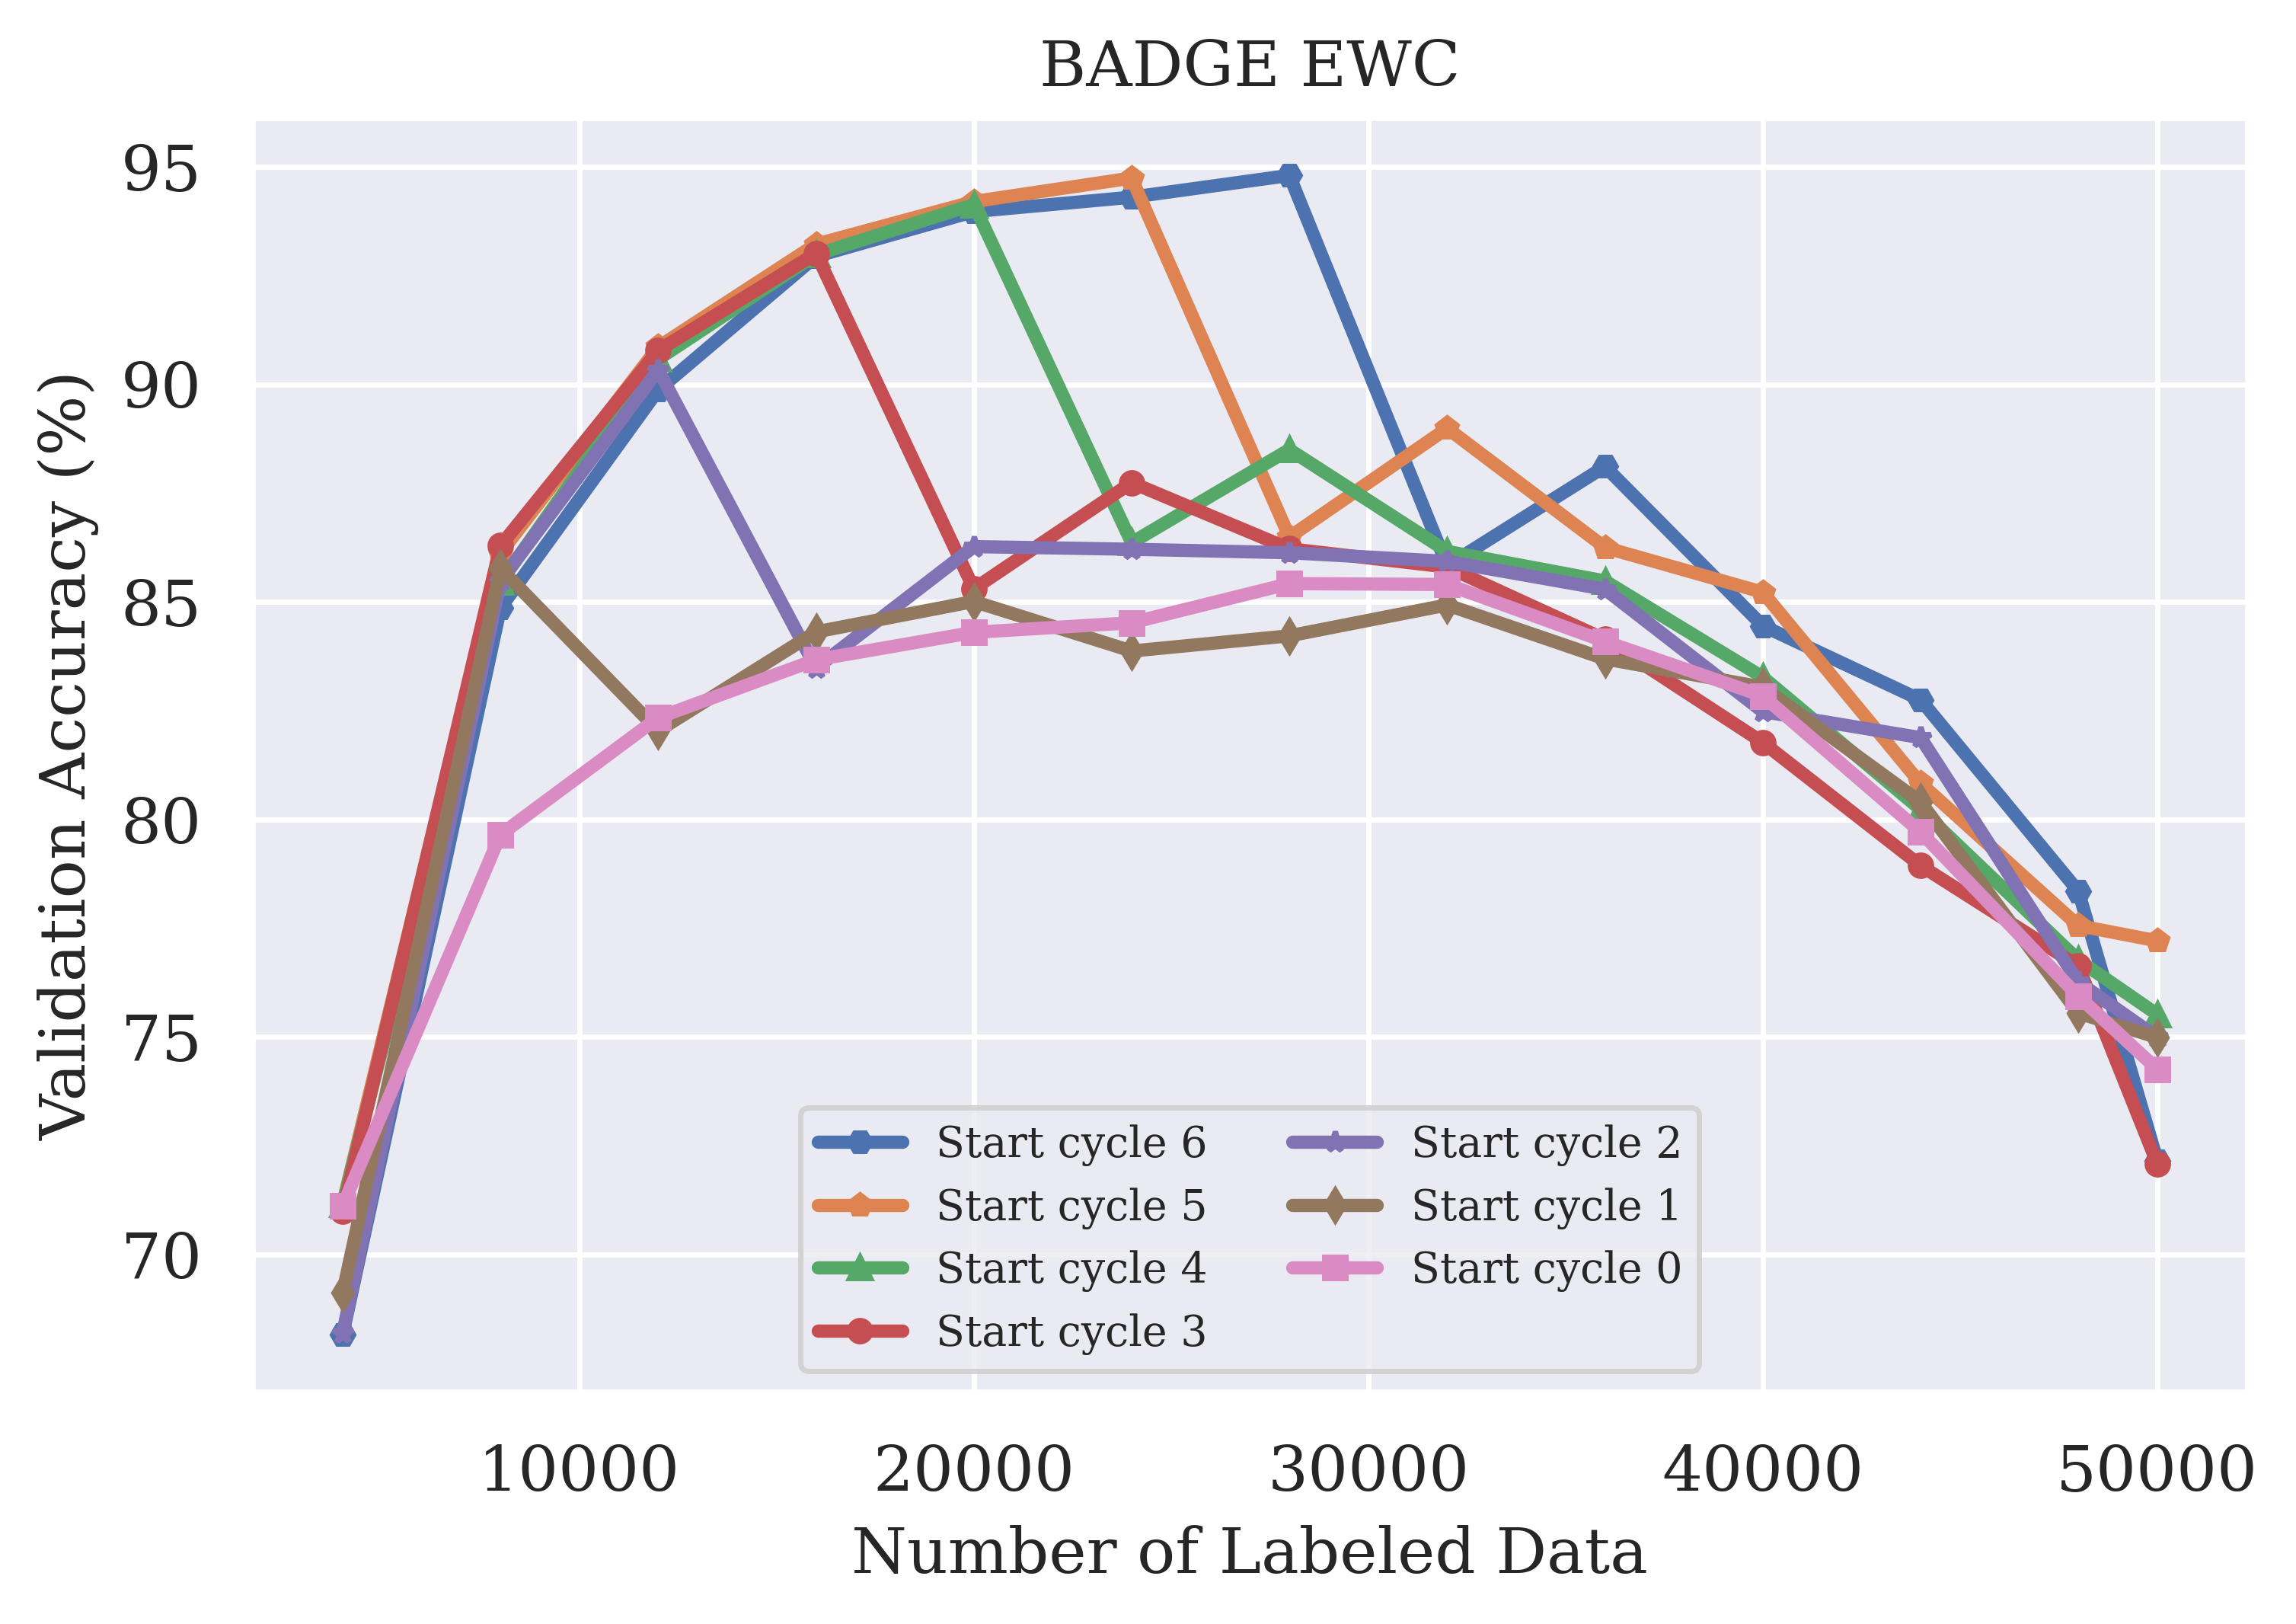
\includegraphics[width=0.45\linewidth]{images/results_CAL/delayed_start_badge_ewc.png} \hfill
    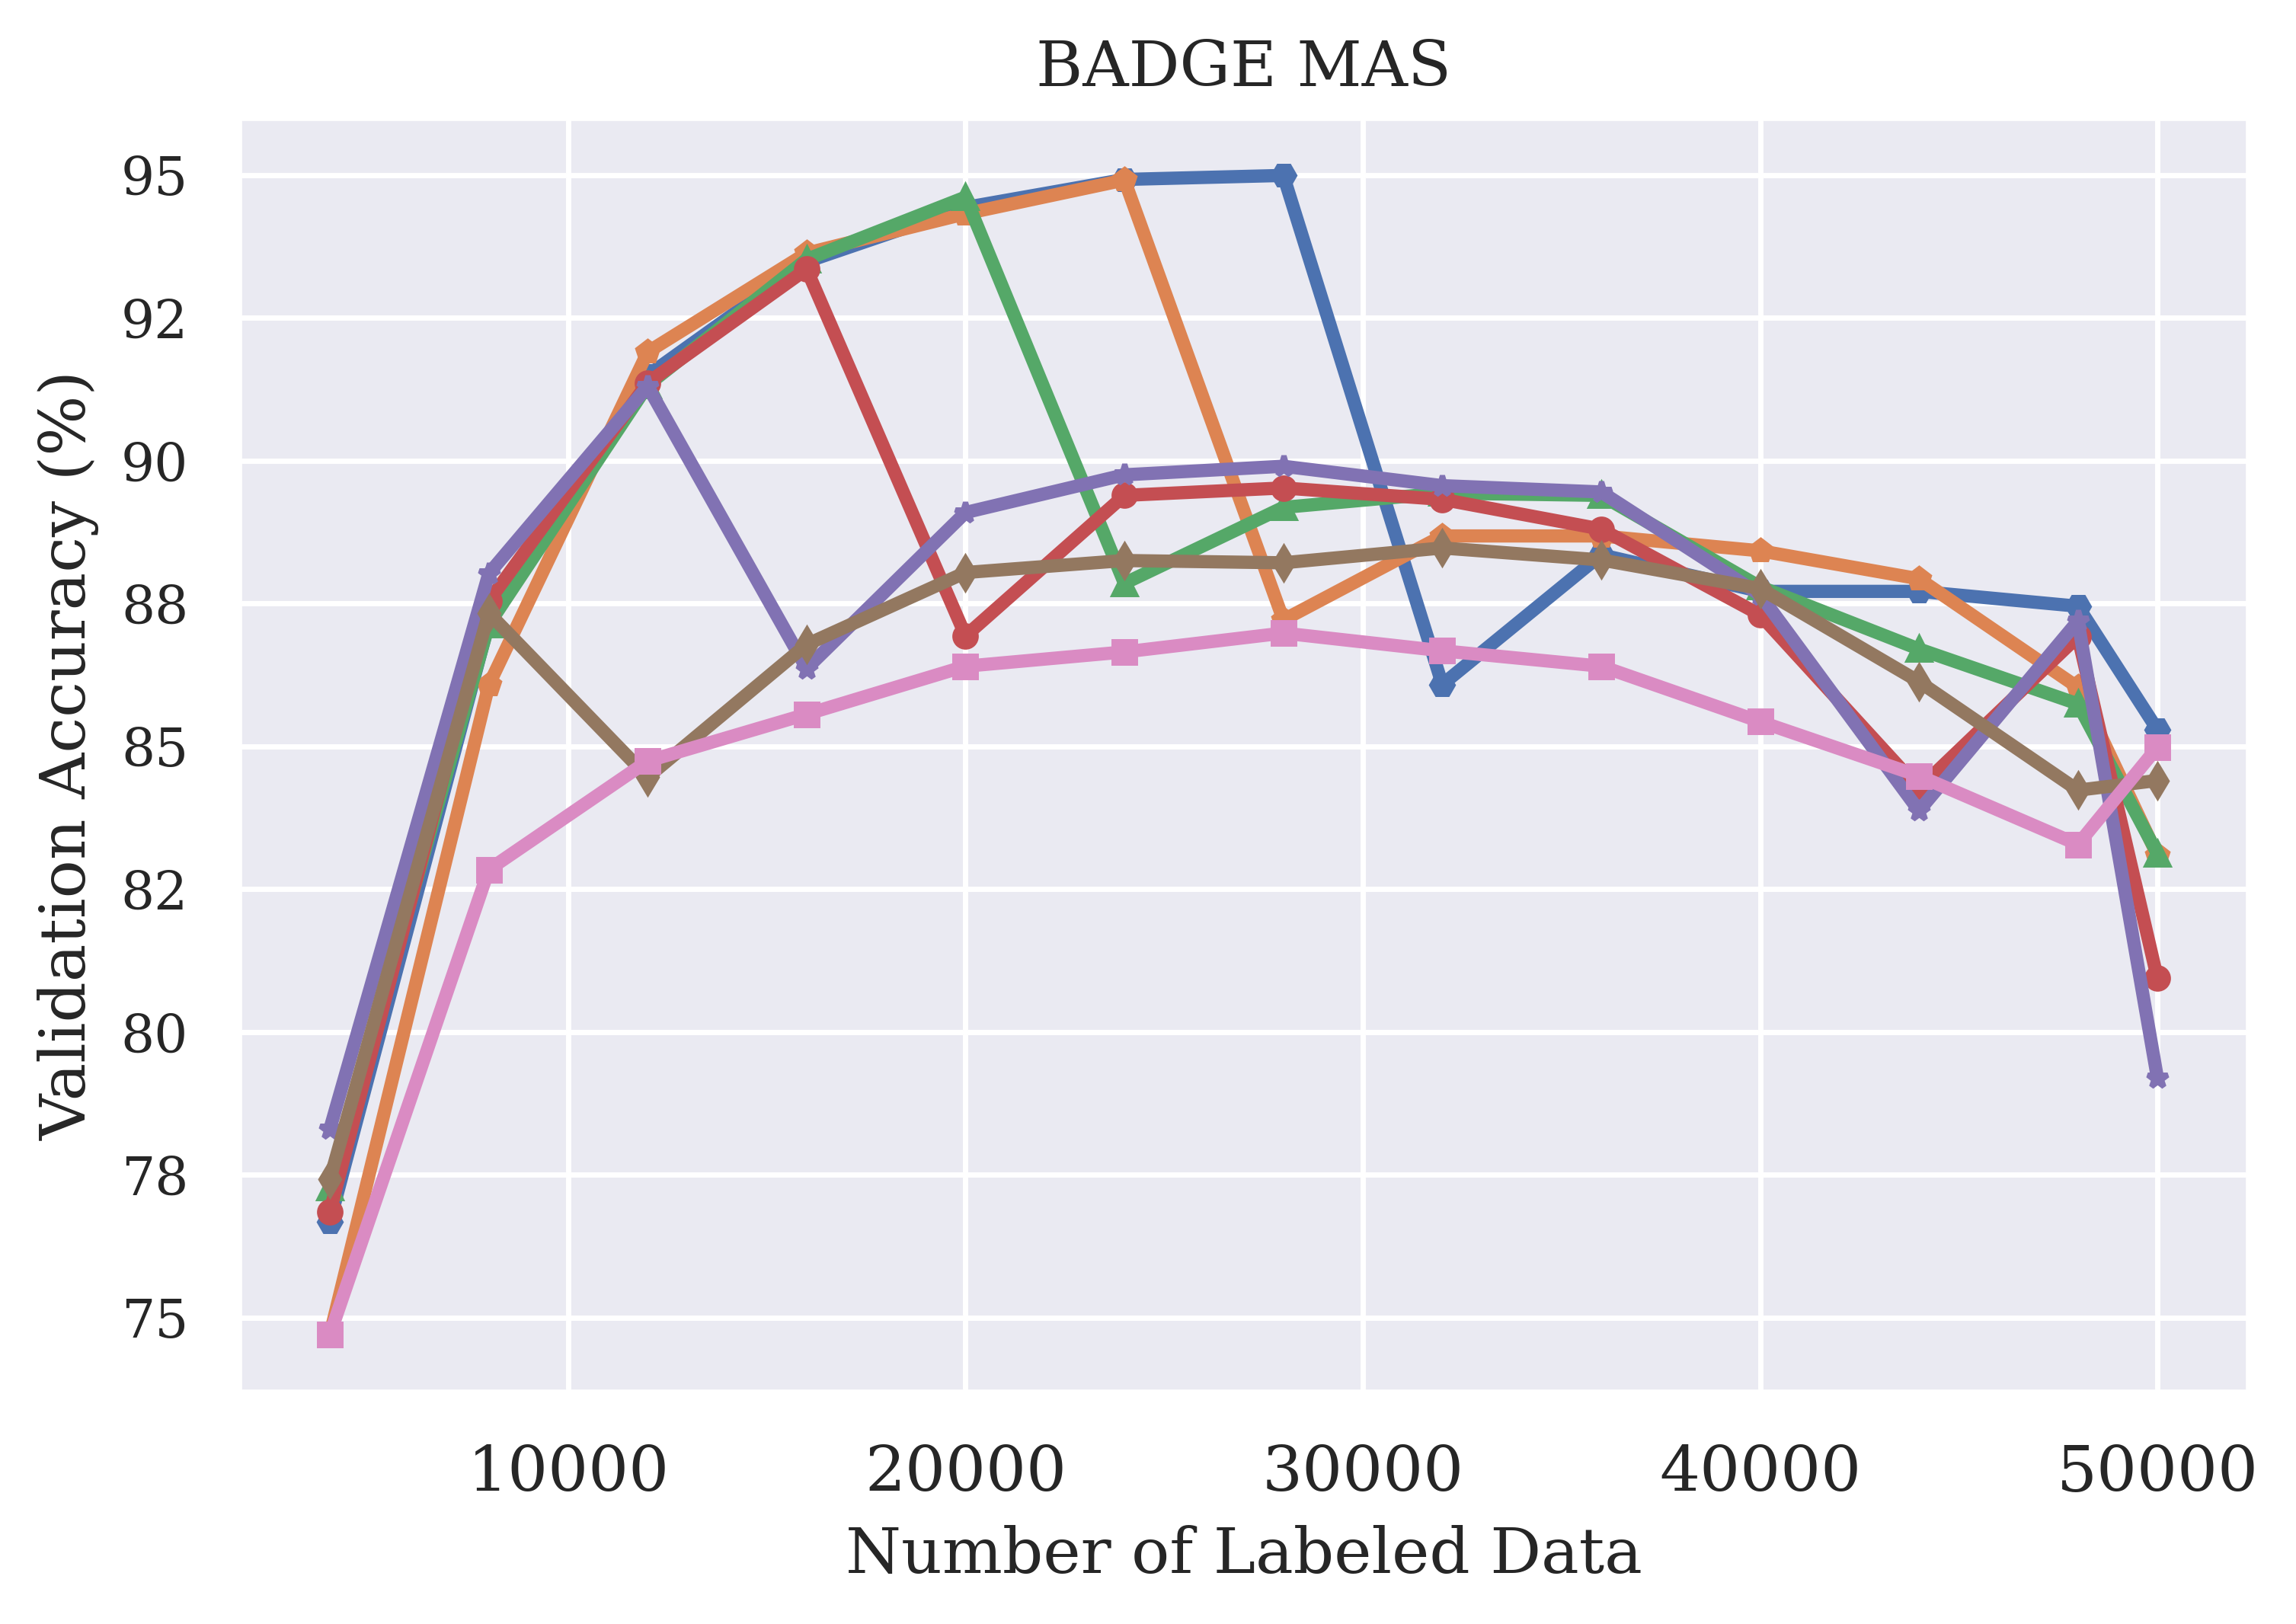
\includegraphics[width=0.45\linewidth]{images/results_CAL/delayed_start_badge_mas.png}
    \caption{Comparison of validation accuracy for a delayed start of Continual Learning.}
    \label{fig:Evaluation:CAL:DelayedStart}
\end{figure}

\subsubsection{Varying the initialization of the labeled pool}
\label{sec:Evaluation:CAL:Initialization}
Motivated by the findings from the previous section, we wonder if the initialization of the labeled pool impacts the validation accuracy of the continual learning strategies.
Beck et al. \cite{beck2021effective} show that using a facility location selection \cite{iyer2021submodular} yields better validation accuracy when training on the initial labeled pool.
We, therefore, test the effect of an initialization using facility location selection compared to our random initialization. As our active learning strategy, we use \gls{badge} with
a batch size of 4000 and \gls{mas} as our continual learning method. The results of the experiment can be found in figure \ref{fig:Evaluation:Results:CAL:FLinit}. While the facility
location approach performs better than random initialization, the difference is marginal. Interestingly, the validation accuracy of the facility location approach is lower than
random initialization in the first iteration. The most significant drawback of the facility location initialization is its resource intensity. Initialization with facility
location takes about 24 hours to complete and requires more than 100GB of memory (compared to <10 seconds and <2GB) for CIFAR-10 using the implementation provided by Beck et al.
\cite{beck2021effective}. \par

\begin{figure}[h]
    \centering
    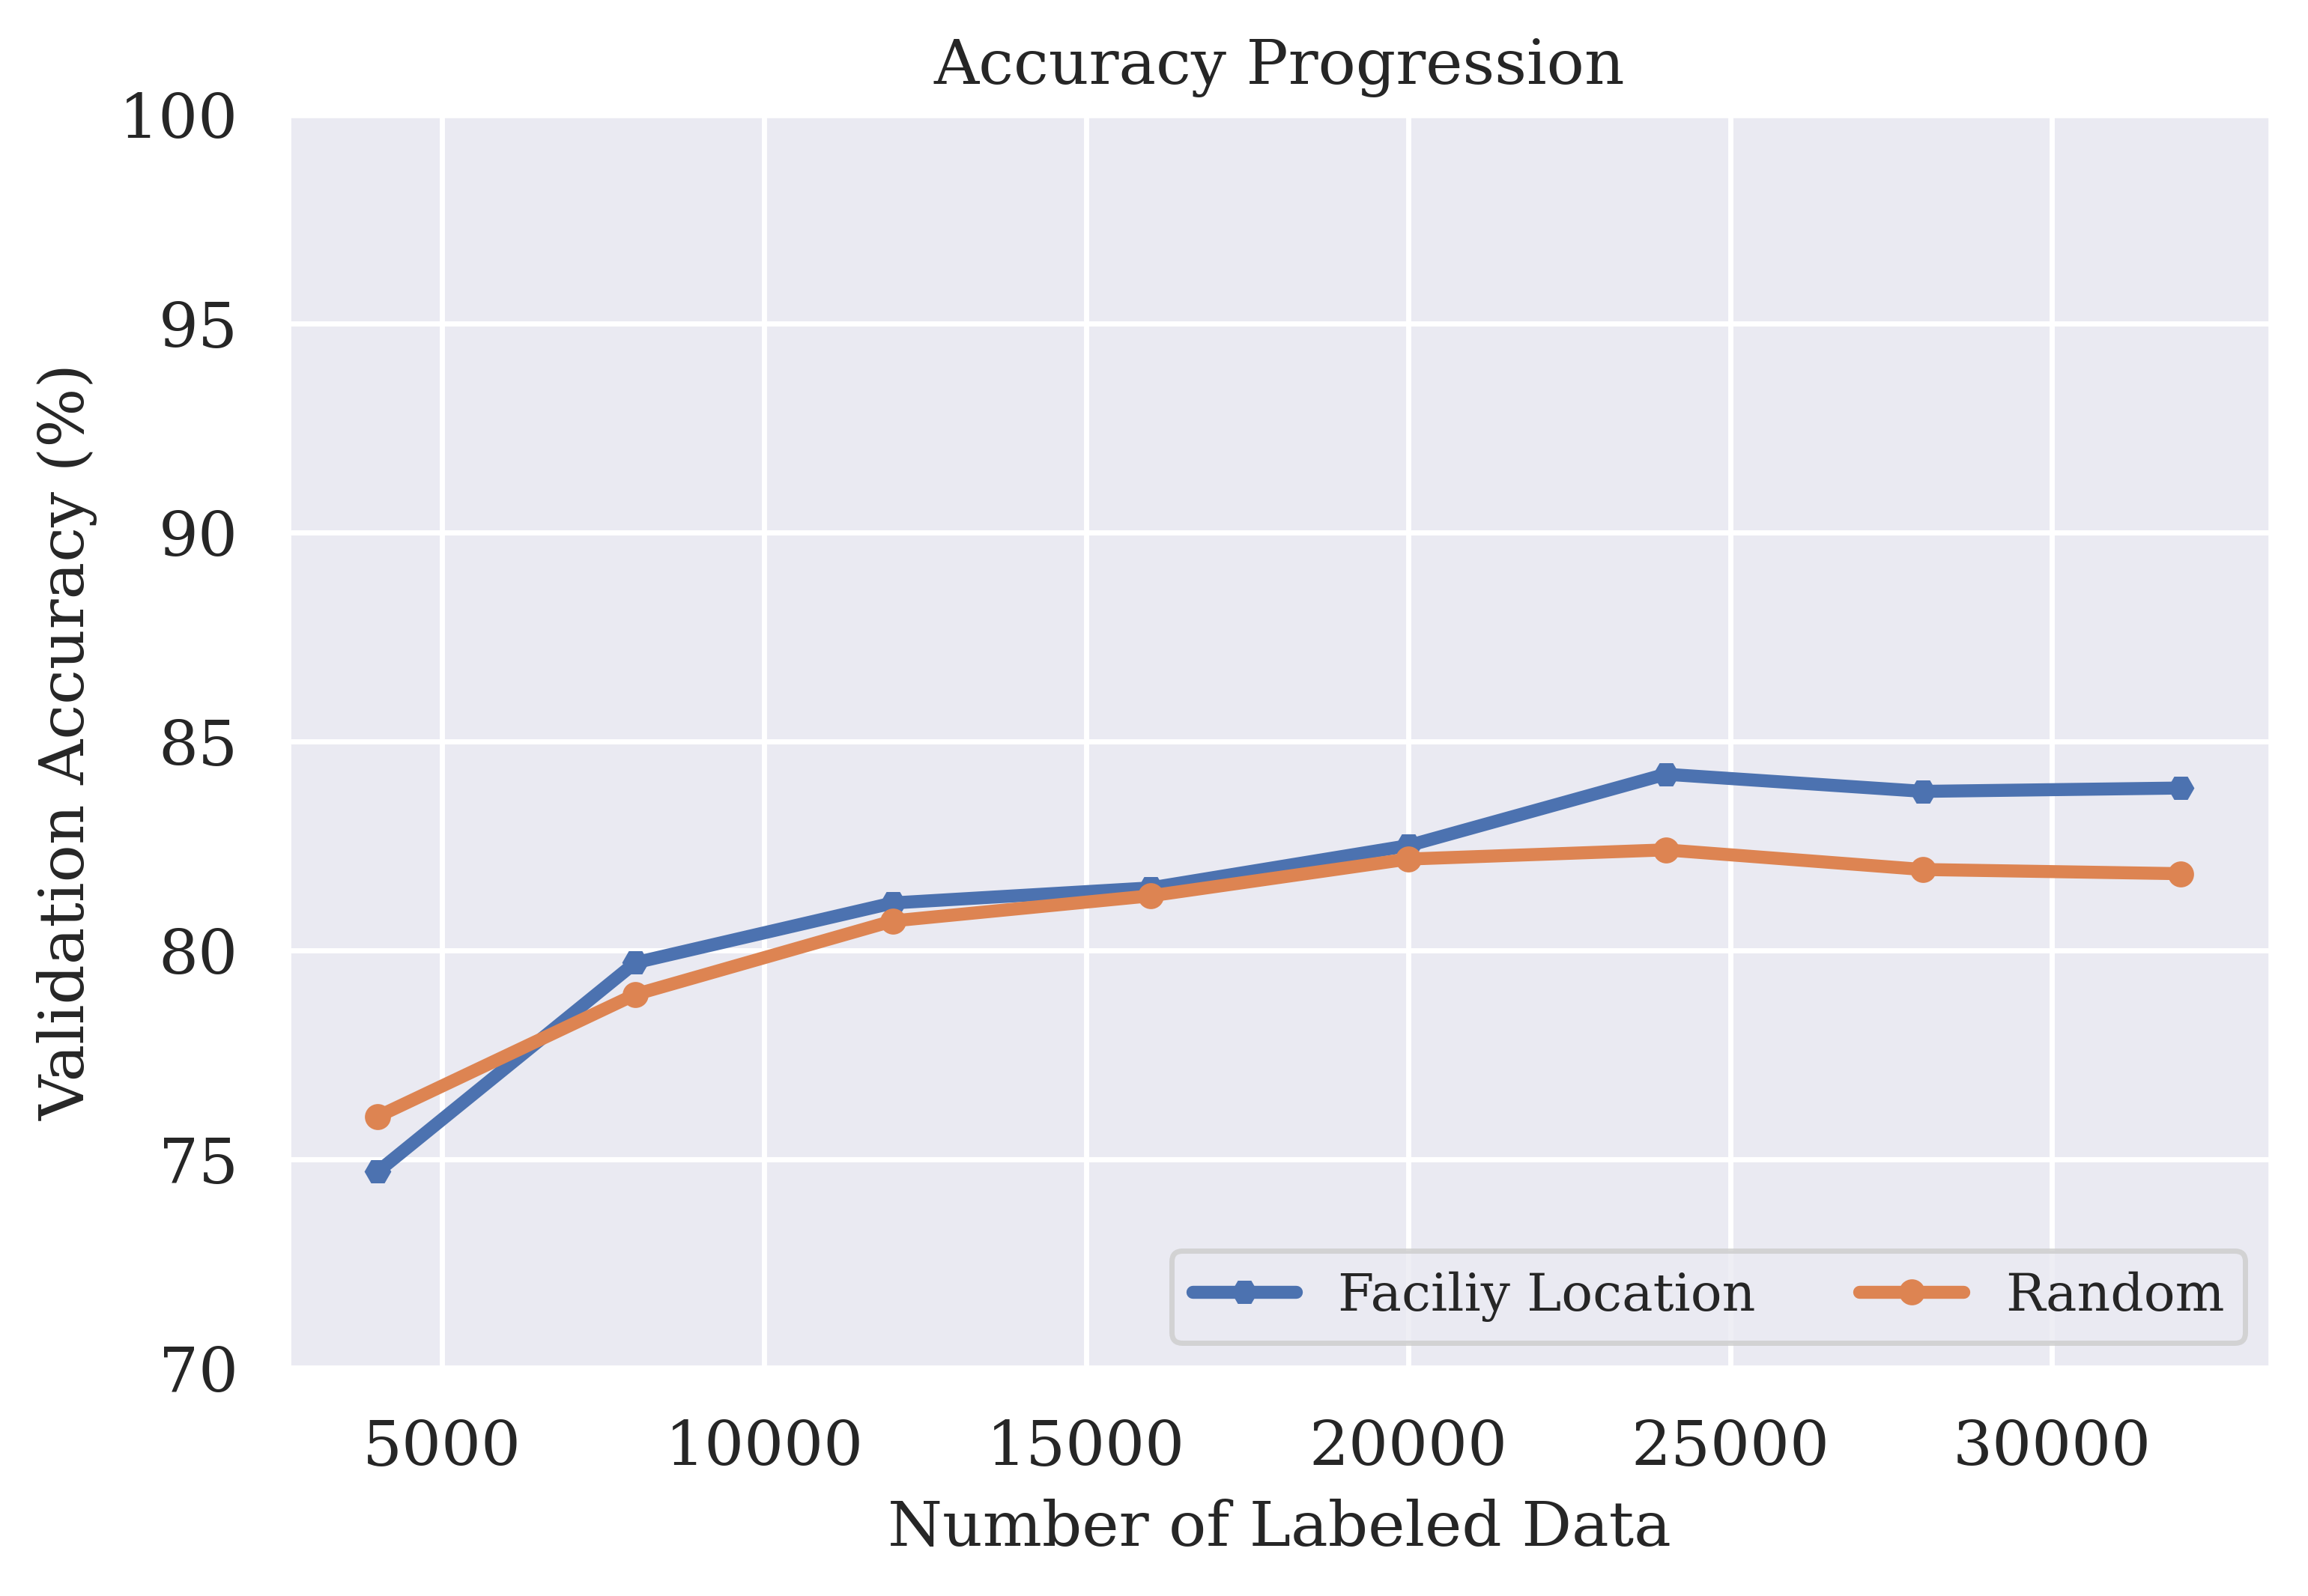
\includegraphics[width=0.6\linewidth]{images/results_CAL/Facility_location_init.png}
    \caption{Comparison of validation accuracy for facility location initialization and random initialization}
    \label{fig:Evaluation:CAL:FLinit}
\end{figure}


\subsection{Replay Continual Learning}
\label{sec:Evaluation:CAL:Replay}
In section \ref{sec:Methodology:ReplayStrategy}, we introduced a custom replay strategy for Continual Active Learning. Using our replay strategy is motivated by the main
finding of section \ref{sec:Evaluation:Results:CAL:BatchSize}: the validation accuracy increases with increased batch size. In this set of experiments, we use the active
learning strategy CoreSet and vary the batch size as well as the size of the replay buffer. Moreover, we investigate the effect of CoreSet selection in the replay buffer
compared to random selection. We present our results in figure \ref{fig:Evaluation:CAL:Replay}. When varying the batch size and buffer size, we notice that increasing either
or both of them yields a higher validation accuracy. However, our replay strategy does not outperform the naive approach when using the same amount of training data
(i.e., batch size + replay buffer size for the replay strategy and batch size for the naive approach). This leads us to believe that the most decisive factor for the performance
of continuous active learning is the amount of training data. For further reasoning, we refer to section \ref{sec:Evaluation:Results:CAL:BatchSize}. \par
To evaluate the importance of CoreSet selection in the buffer compression process, we compare the validation accuracy of our replay strategy when using CoreSet selection and
random selection. We notice that the validation accuracy remains mostly the same for both buffer compression methods, apart from the last 15000 samples, where CoreSet selection
outperforms random selection. This is because the first 25,000 samples queried are informative enough to increase or maintain validation accuracy. Therefore, using random or
CoreSet selection does not influence the validation accuracy at the beginning of the experiment. In the end, however, CoreSet selection ensures that the buffer contains
enough informative samples while random selection does not.  \par


\begin{figure}[h]
    \centering
    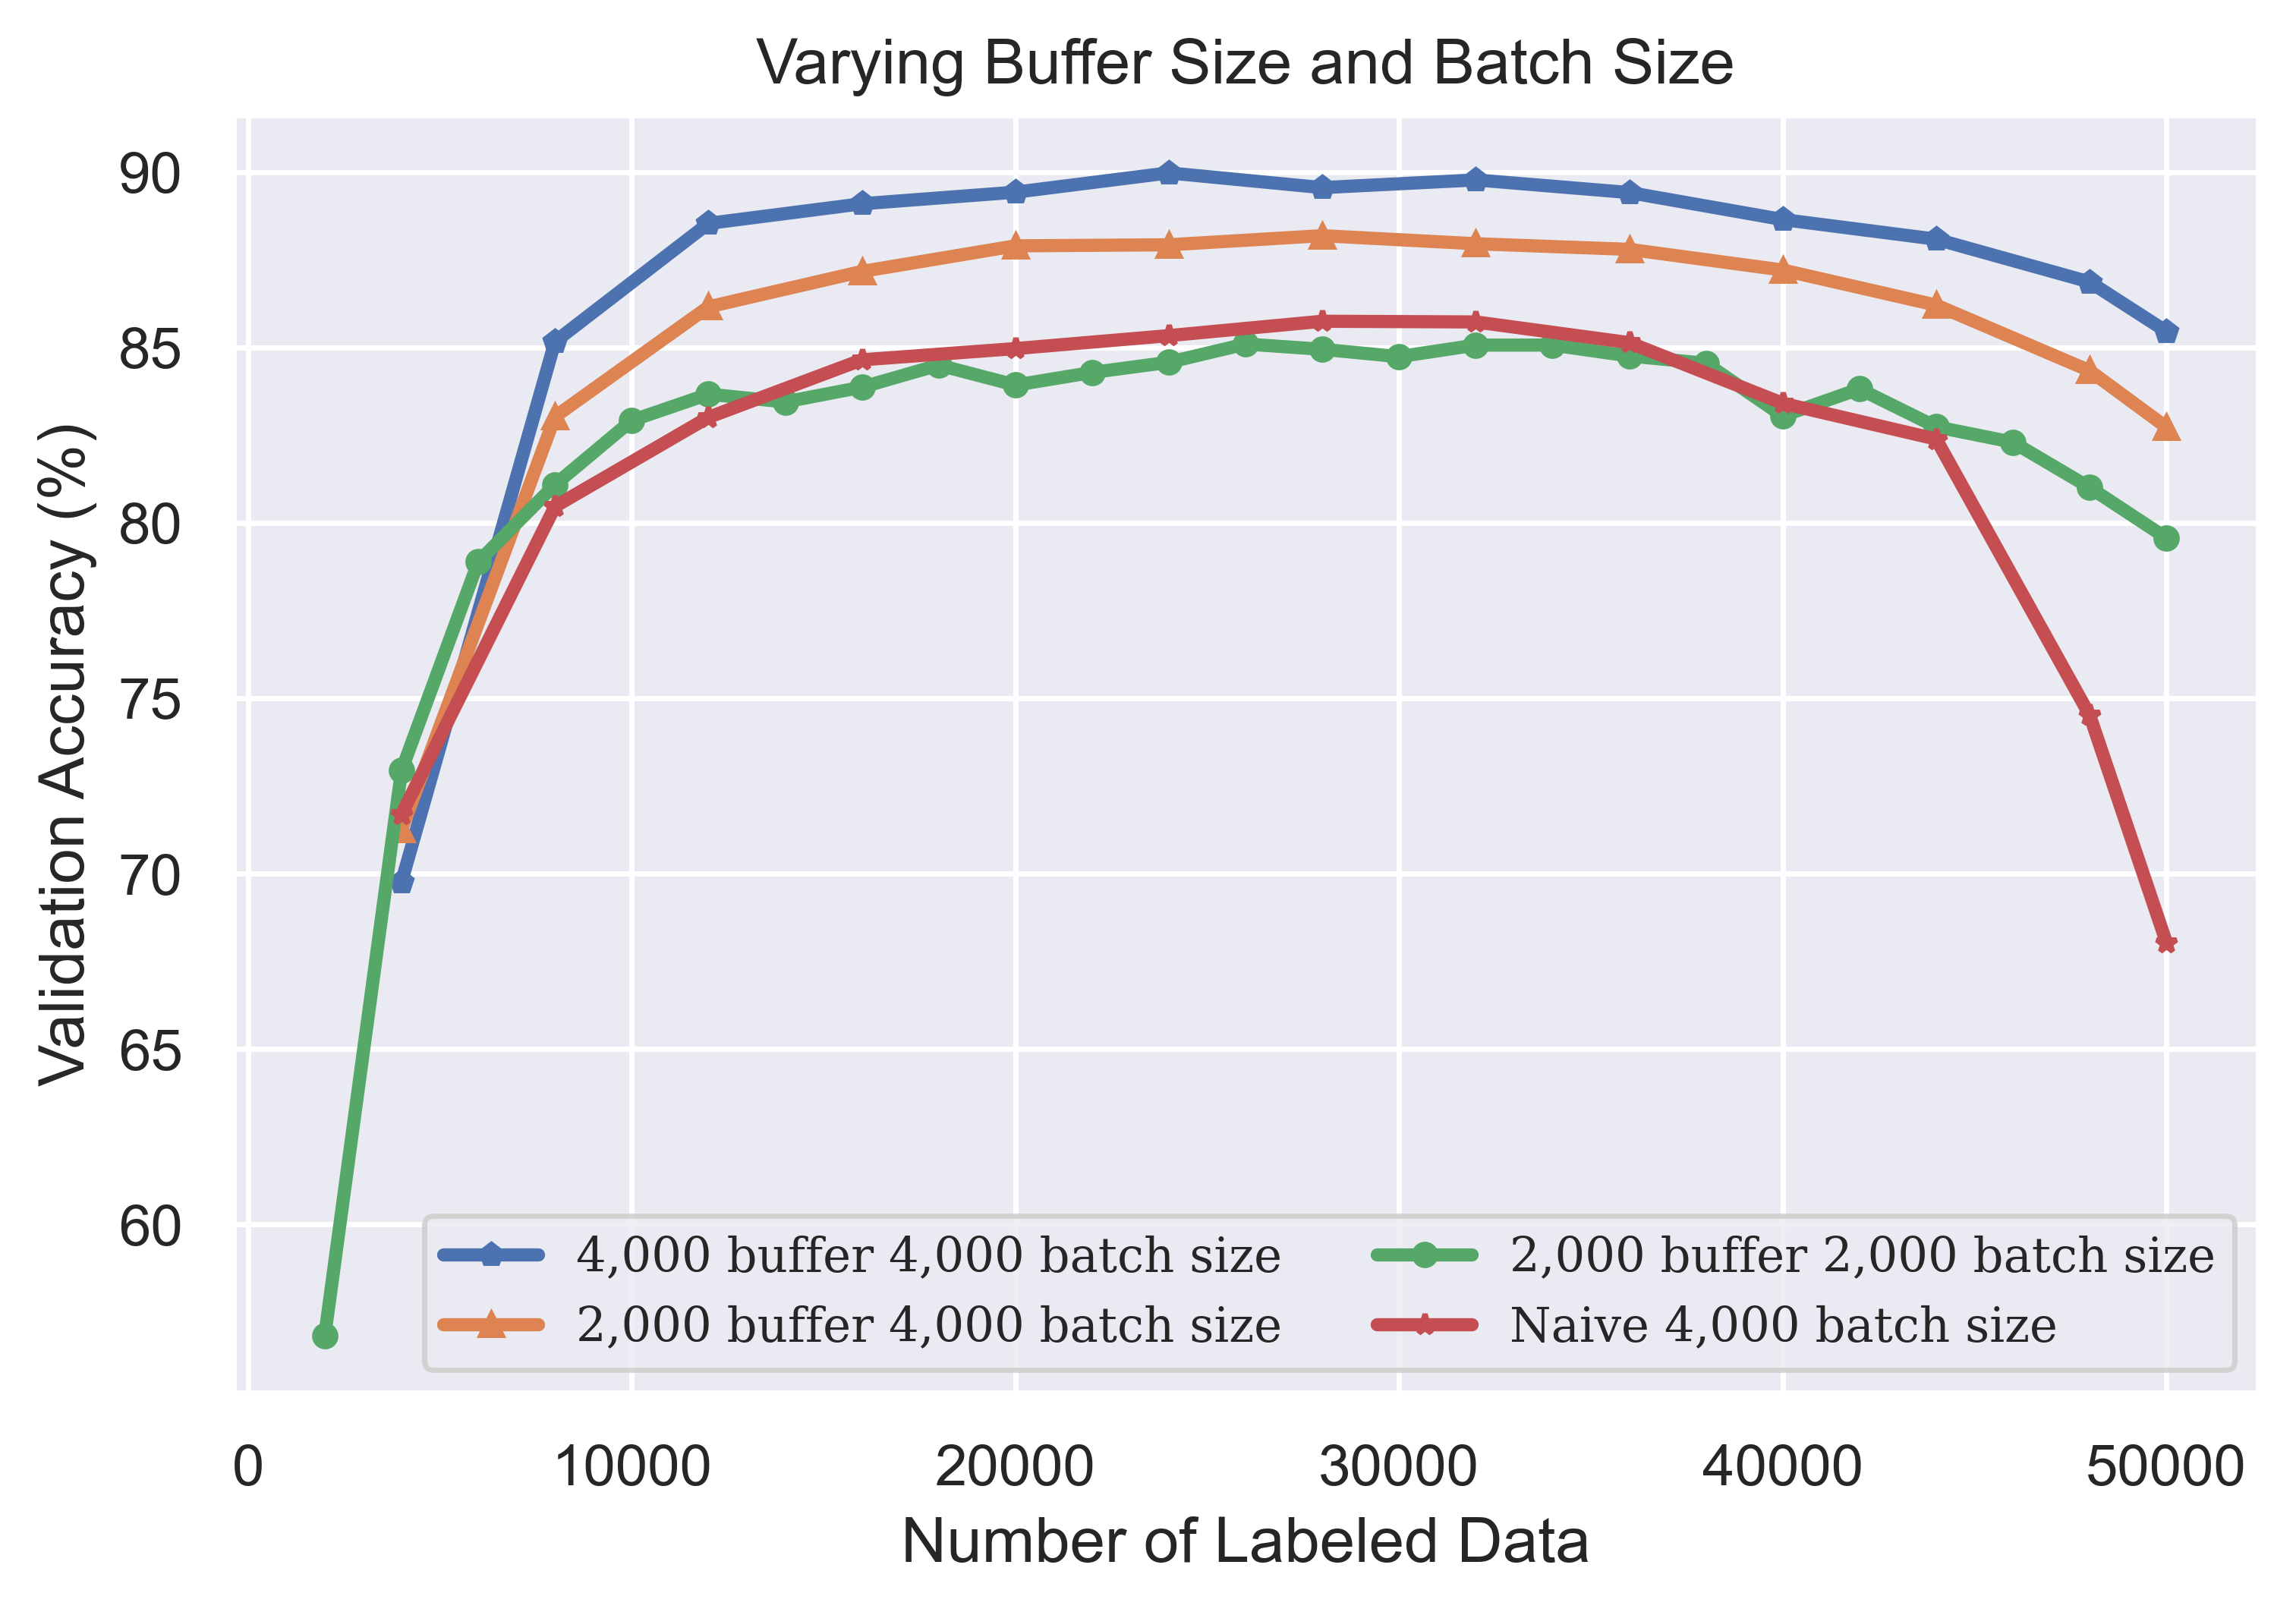
\includegraphics[width=0.45\linewidth]{images/results_CAL/replay_varying_batch_size.png} \hfill
    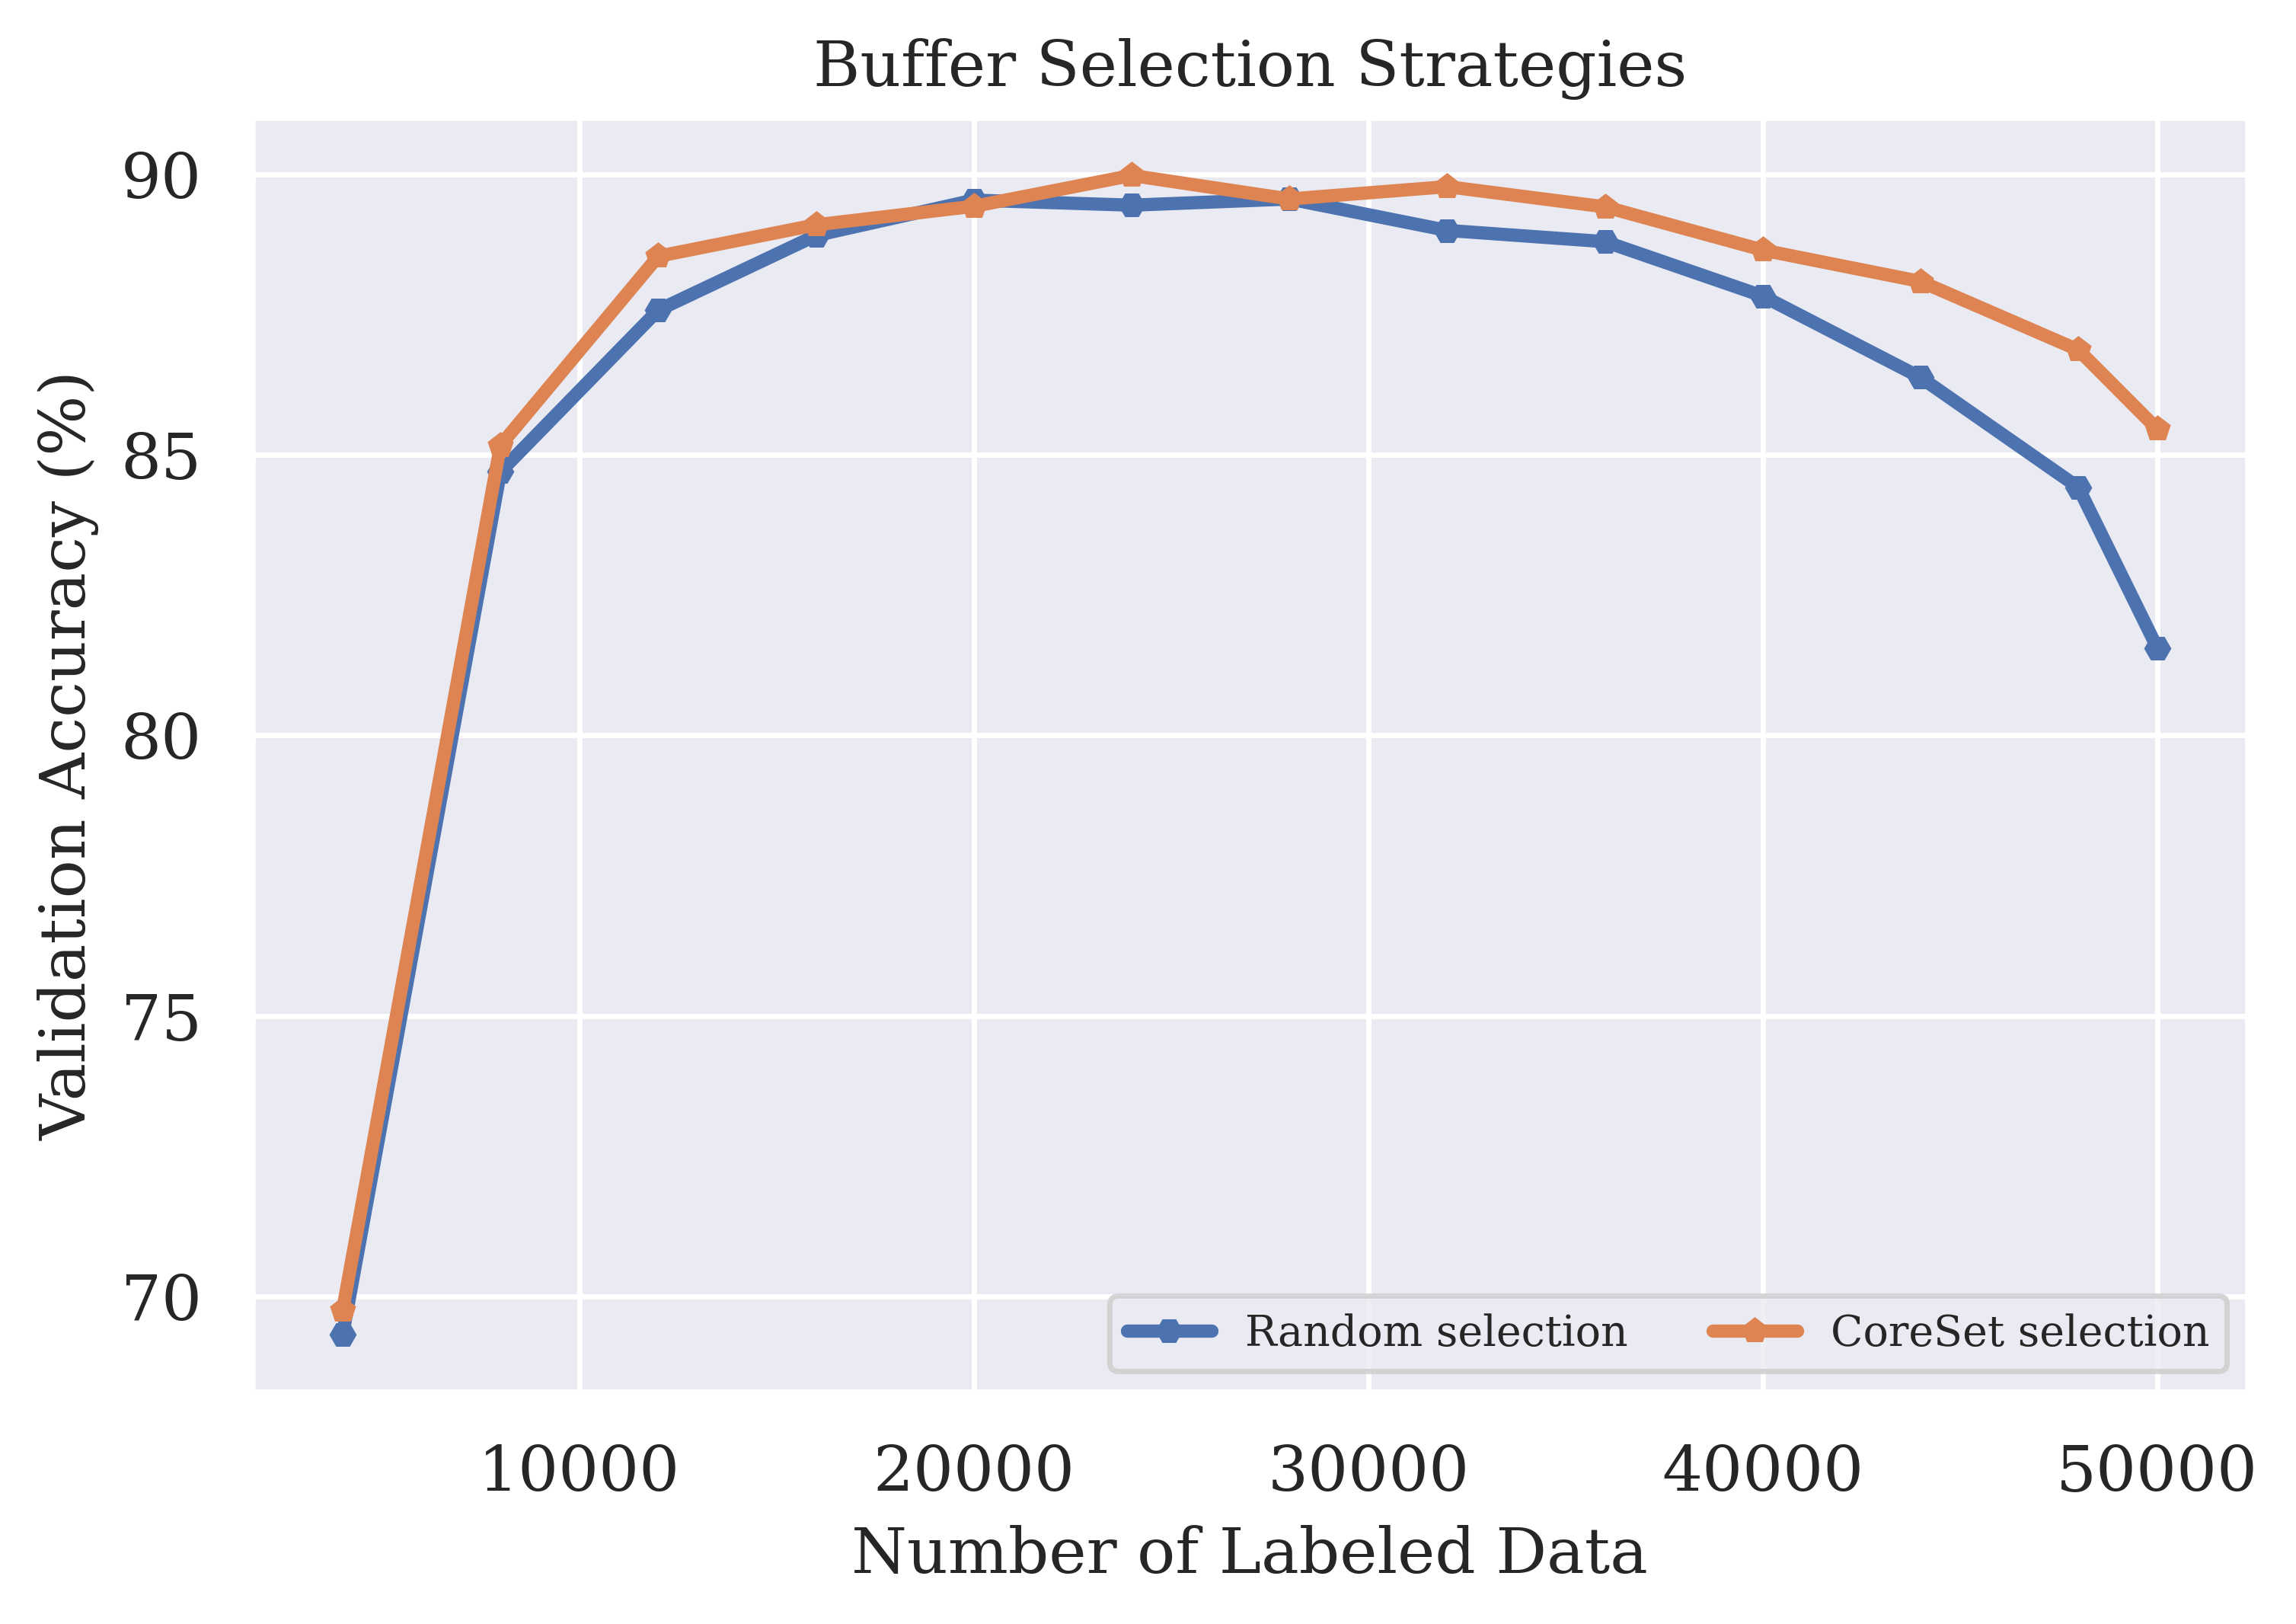
\includegraphics[width=0.45\linewidth]{images/results_CAL/replay_buffer_selection.png}
    \caption{Experiments with our replay strategy}
    \label{fig:Evaluation:CAL:Replay}
\end{figure}

The execution time of our replay strategy is given in table \ref{fig:Evaluation:CAL:Replay_Time}. We notice that the buffer size is the main driver of execution time. This is because
we replay the entire buffer in each iteration, meaning that we train on $\frac{n}{b} \cdot \text{buffer size}$ additional samples, where $n$ is the number of iterations and $b$ is
the batch size. The batch size does not execution time because it does not influence the total number of samples trained on. \par

\begin{table}[h]
    \centering
    \begin{tabular}{c | c  c} 
        Batch size & Buffer size & Execution time\\ 
        \hline 
        4,000 & 4,000 & 121 \\
        4,000 & 2,000 & 107 \\
        2,000 & 2,000 & 130 \\
    \end{tabular}
    \caption{Comparison of execution time using the replay strategy in combination with CoreSet}
    \label{fig:Evaluation:CAL:Replay_Time}
\end{table}


\subsection{Exemplar Rehearsal Continual Learning and Representation-based Active Learning}
\label{sec:Evaluation:CAL:VAAL_AGEM}
Unsatisfied with the results from previous experiments, we decide to implement additional continual and active learning strategies. We perform an extensive literature search,
investigating the suitability of representation-based active learning strategies and continual learning strategies from the exemplar rehearsal category in the summary paper
by Mundt et al. \cite{mundt2020wholistic}. The active learning strategy which we implement is \gls{vaal} \cite{sinha2019variational}, and the continual learning strategy is
\gls{a-gem} \cite{chaudhry2018efficient}. We decide to implement \gls{vaal} because it is the only representation-based active learning strategy that consistently performs
better than random sampling (apart from CoreSet, which we have already implemented). We choose to implement \gls{a-gem} as our continual learning strategy as it
is one of the few exemplar rehearsal strategies applicable to (semi-) supervised learning (many other strategies focus on reinforcement learning). Furthermore, \gls{a-gem}
is computationally efficient and demonstrates strong performance in the experiments by Chaudhry et al. \cite{chaudhry2018efficient}. \par
First, we analyze the performance of \gls{vaal} as an active learning strategy. We run \gls{vaal} with a batch size of 4,000 and compare it to Random and CoreSet. We choose
Random because it is the baseline for active learning strategies and CoreSet because it is among the best performing active learning methods used before. The results are depicted in the left plot in figure \ref{fig:Evaluation:Results:CAL:VAAL}. While \gls{vaal} outperforms random sampling by a large margin, it is outperformed by about the
same margin by CoreSet. To ensure that the results are not due to a suboptimal hyperparameter choice, we run \gls{vaal} training \gls{vae} and discriminator for 20 epochs in
one run and 100 epochs in another. Because we are interested in the performance of \gls{vaal} in our continual active learning setting, we use continual active learning with
a batch size of 4,000 and the continual learning strategy Naive. We present the results in the right plot of figure \ref{fig:Evaluation:Results:CAL:VAAL}.
Surprisingly, the training time of the discriminator and \gls{vae} marginally impacts validation accuracy. If anything, the validation accuracy is higher when training for
20 epochs. We attribute the performance gap between CoreSet and \gls{vaal} to the fact that the samples from the labeled and unlabeled pool are too similar. This also
explains why training discriminator and \gls{vae} for more epochs does not increase validation accuracy. \par

\begin{figure}[h]
    \centering
    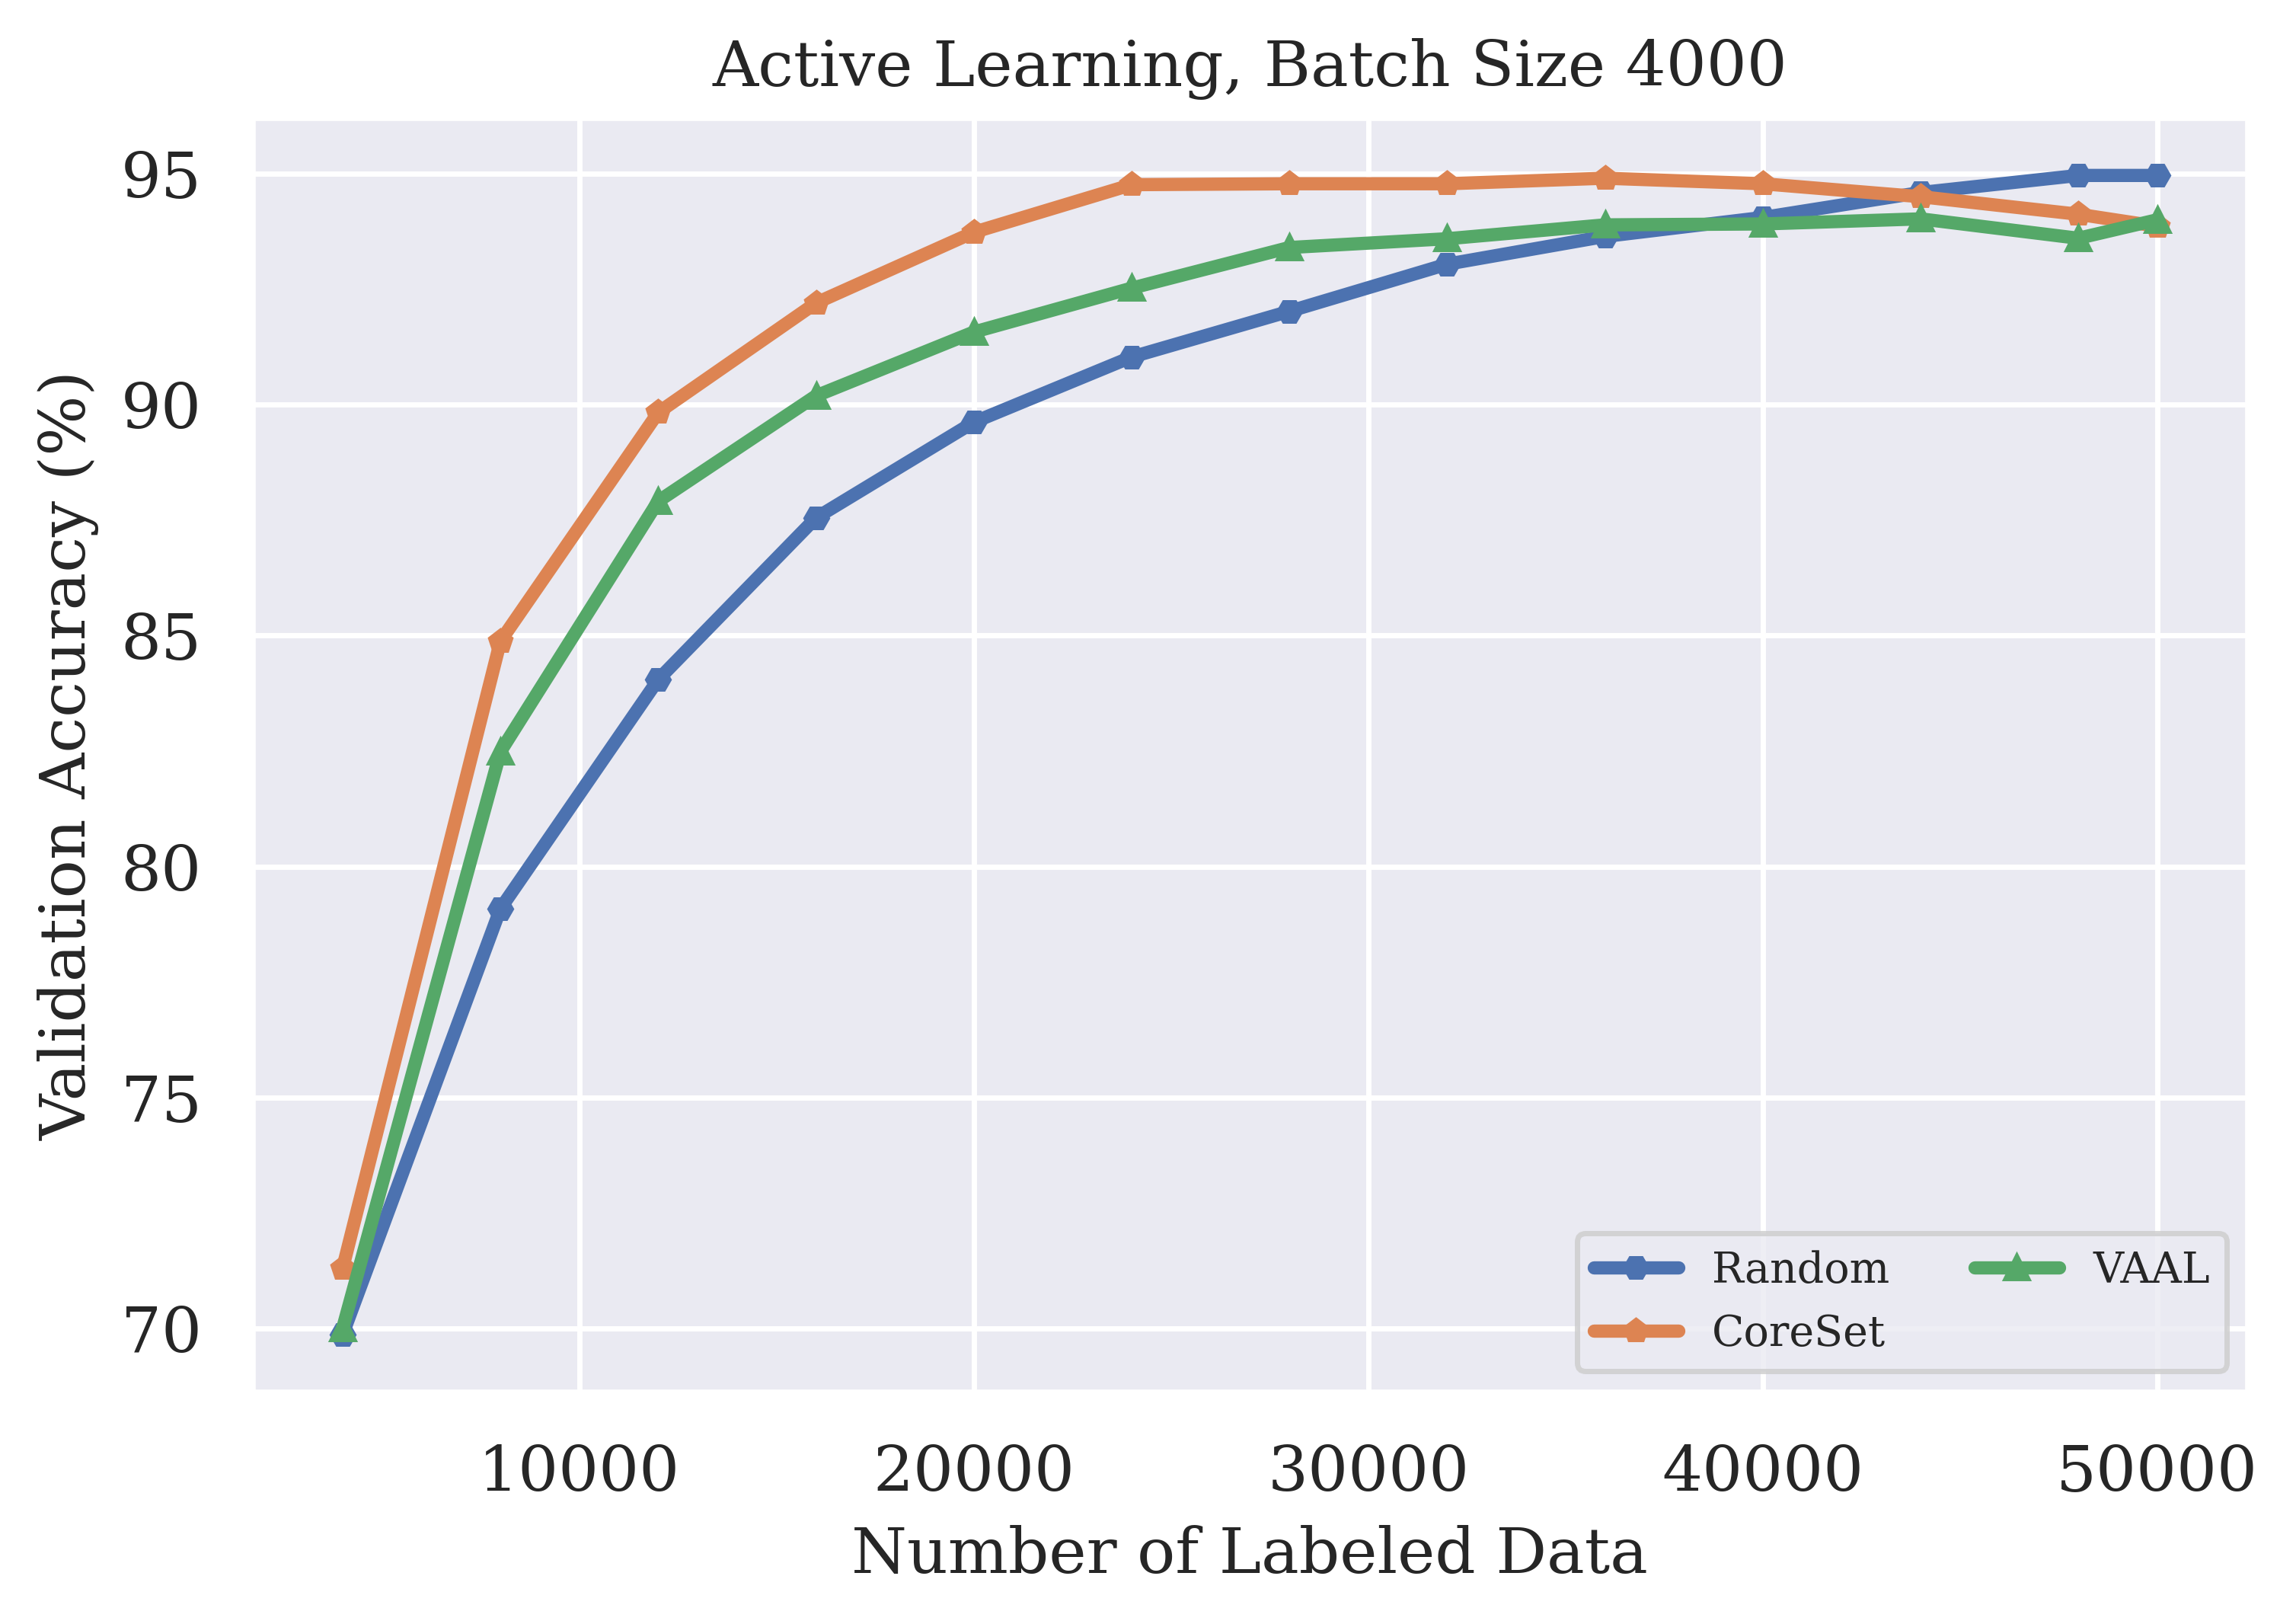
\includegraphics[width=0.46\linewidth]{images/results_CAL/vaal_al.png} \hfill
    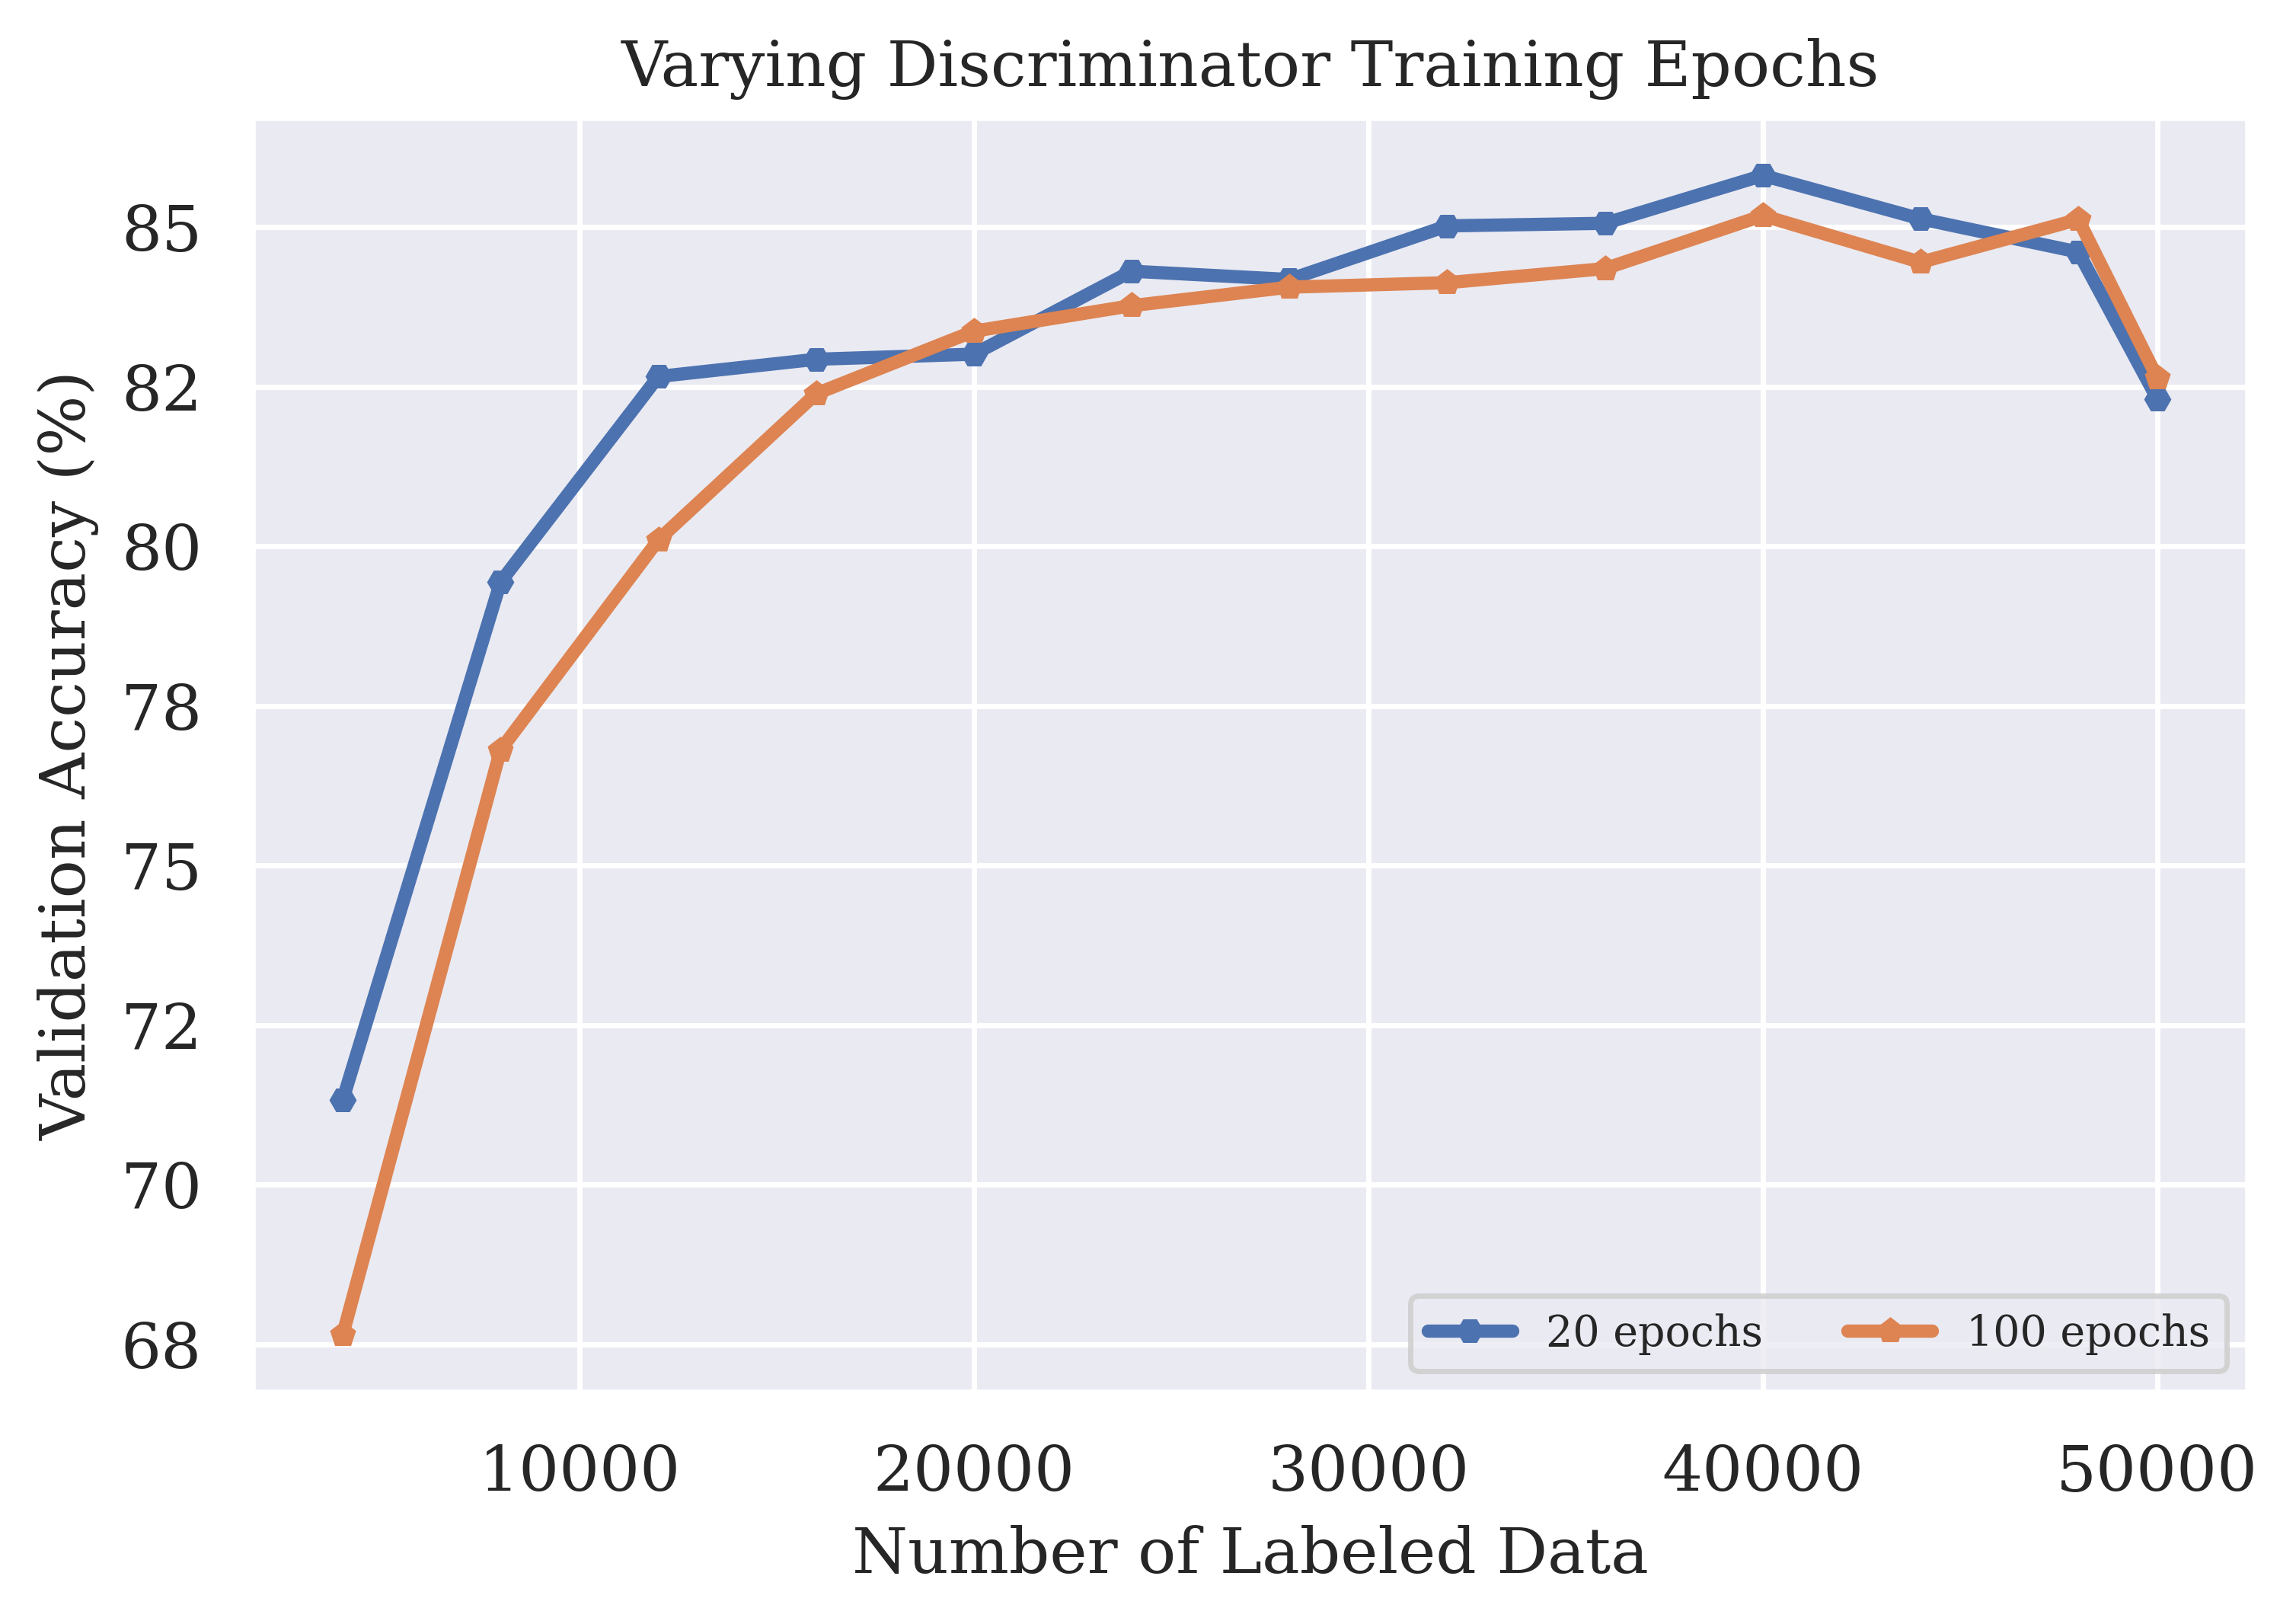
\includegraphics[width=0.46\linewidth]{images/results_CAL/vaal_disc_epochs.png}
    \caption[Continual Active Learning Custom Replay strategy]{Left: Comparing \gls{vaal} to Random and CoreSet.
    Right: Comparison of validation accuracy when varying the training epochs for \gls{vae} and discriminator.}
    \label{fig:Evaluation:CAL:VAAL}
\end{figure}

Next, we experiment with \gls{a-gem}. \gls{a-gem} has two hyperparameters: $S$,  the number of samples randomly drawn from the memory to compute the reference
gradients, and $P$, the number of data points stored in the memory from each task. We run \gls{a-gem} with the Active Learning strategy \gls{lc} and a batch size
of 2,000. To assess the performance of \gls{a-gem}, we compare its validation accuracy to the naive approach. We vary $S$ and $P$ and present our results in the right plot
of figure \ref{fig:Evaluation:Results:CAL:AGEM}. The validation accuracy increases with increased $S$ and $P$ until about 12,000 samples, after which the validation 
accuracy drops for all values of $S$ and $P$. \gls{a-gem} outperforms the naive approach for the first 15,000 samples but is outperformed by Naive for the remainder of
the experiment. \par
After investigating the influence of \gls{a-gem}'s hyperparameters, we compare the combination of \gls{vaal} and \gls{a-gem} to \gls{vaal} and Naive, using a batch size
of 4,000. The results are shown in the left plot of figure \ref{fig:Evaluation:Results:CAL:AGEM}. Although \gls{a-gem} performs worse than the Naive
approach when using \gls{lc}, it outperforms the naive approach when using \gls{vaal} as the active learning strategy. We believe that \gls{a-gem} profits from the 
representation-based sampling of \gls{vaal} and the increased batch size, which explains the improved performance in this setting. \par

%TODO: Hier plots erneuern sodass sie nicht aus powerpoint kommen
\begin{figure}[h]
    \centering
    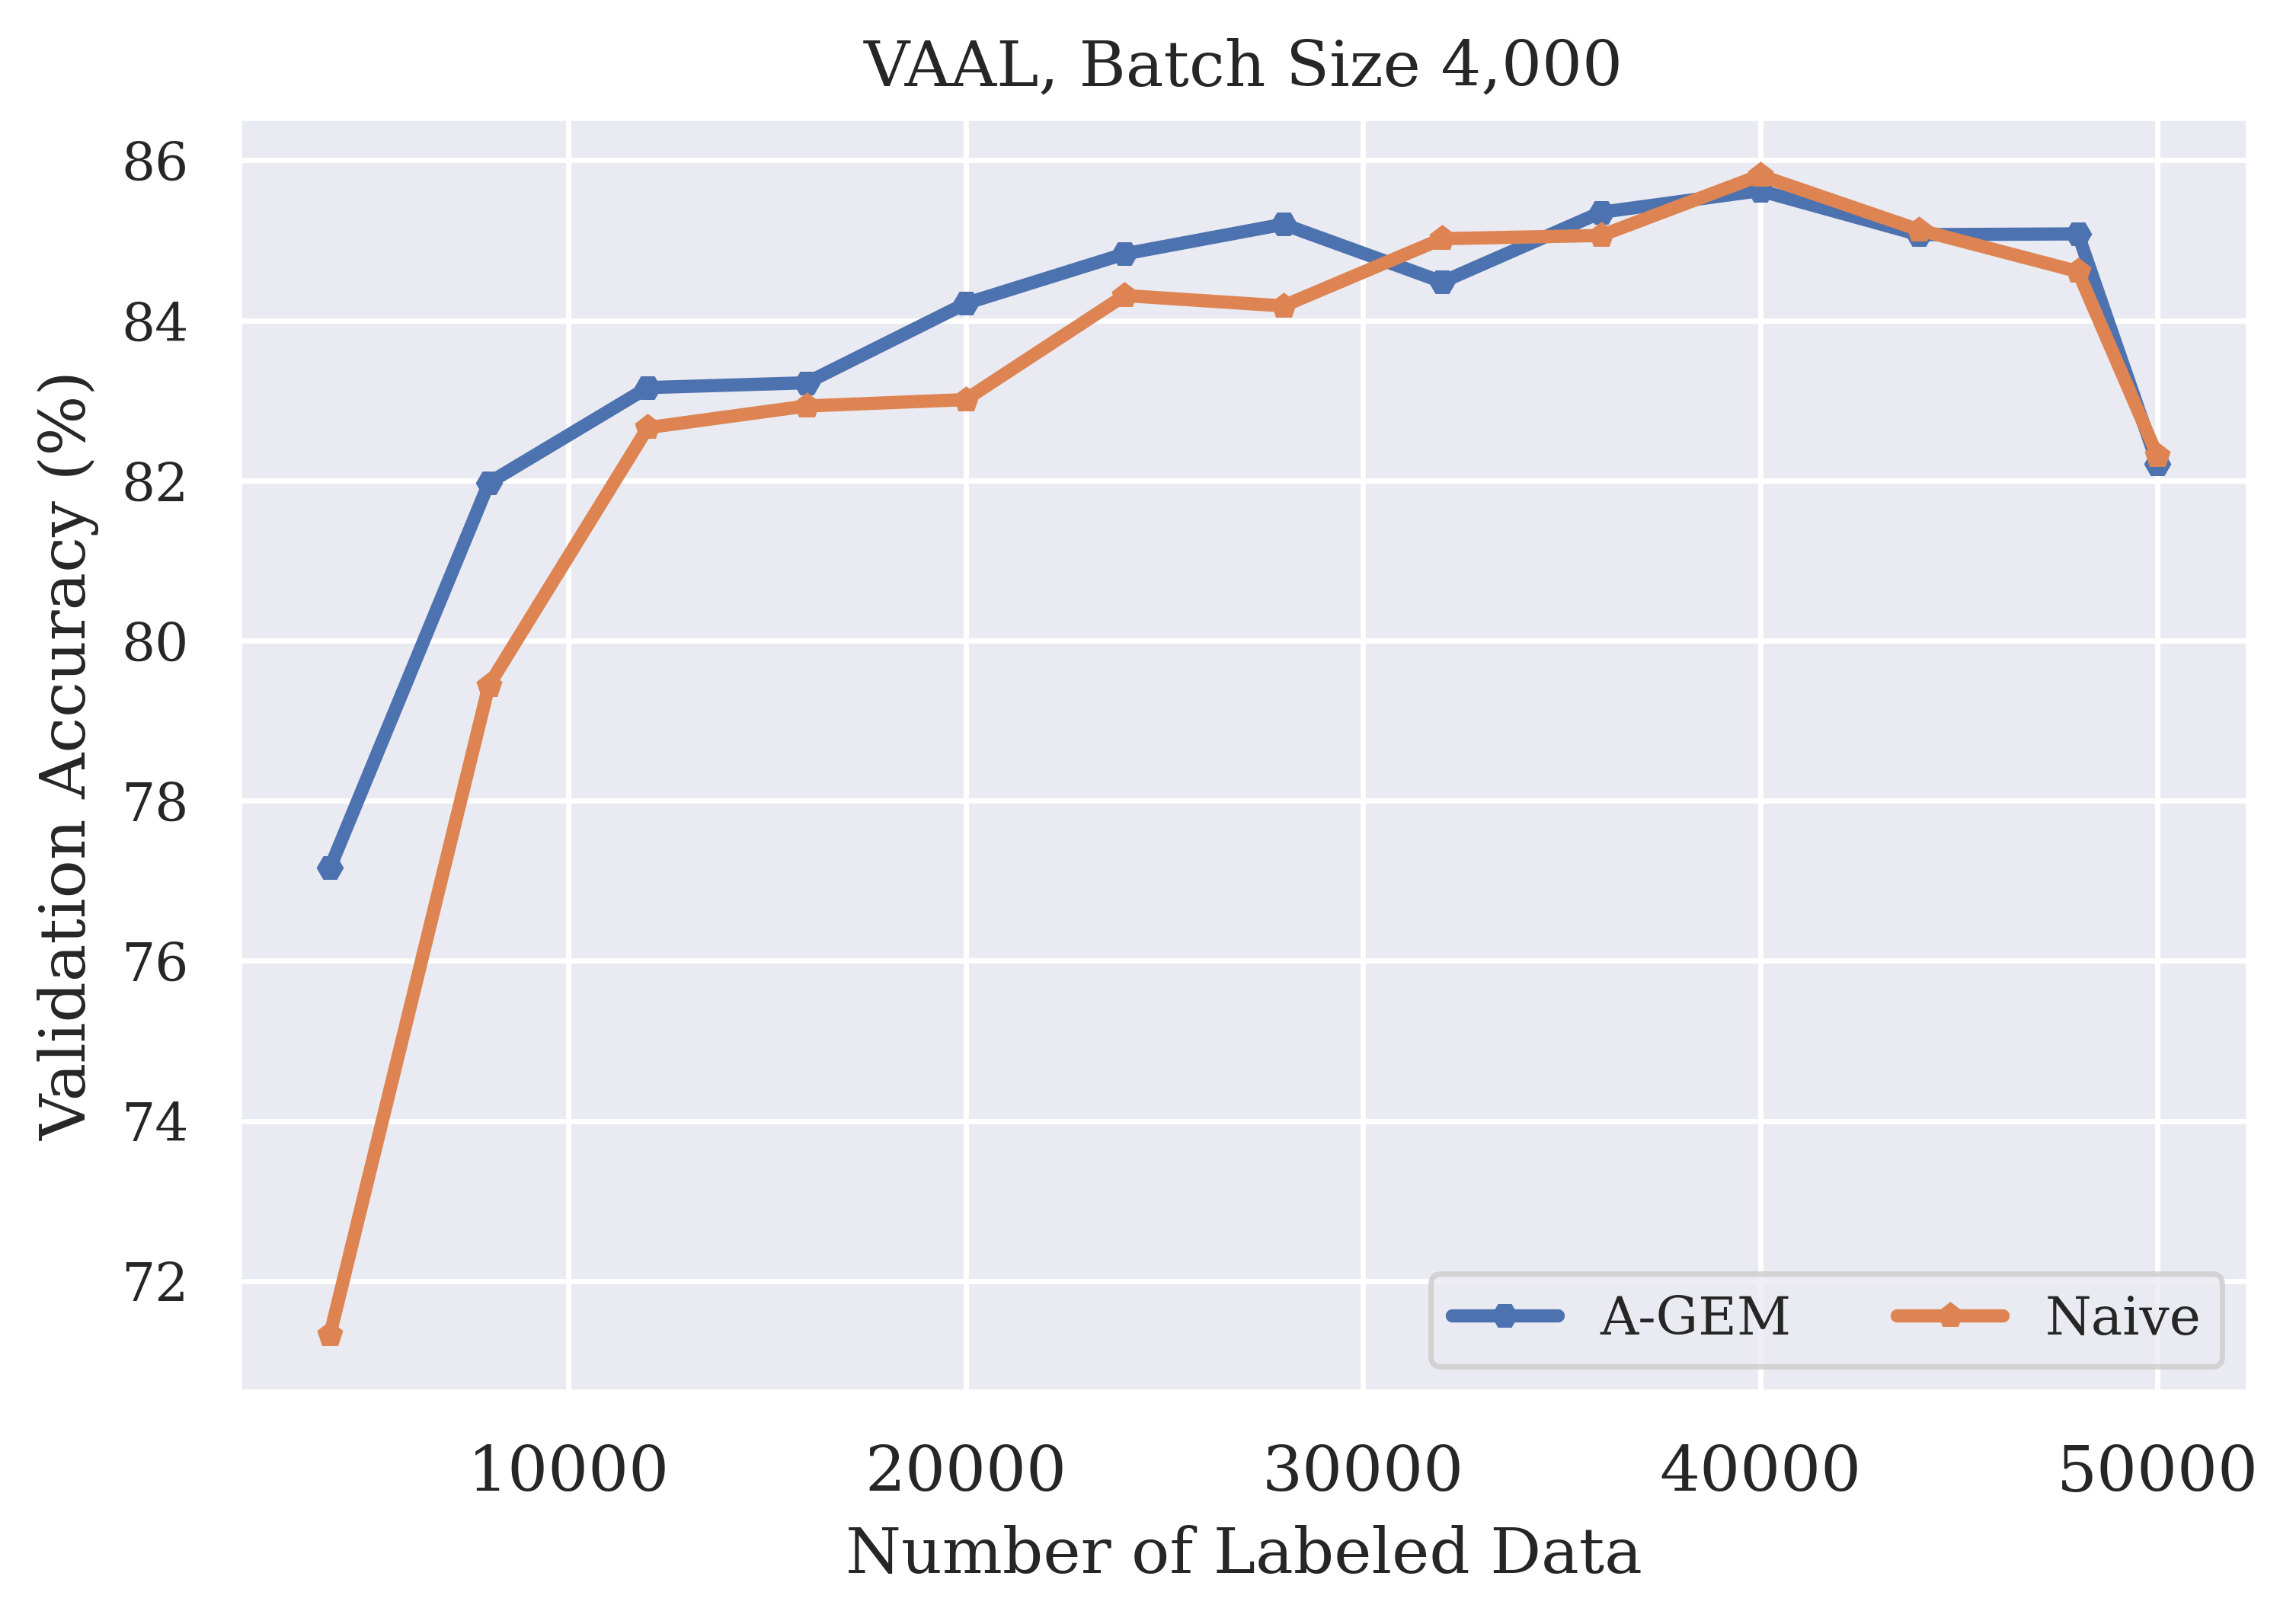
\includegraphics[width=0.48\linewidth]{images/results_CAL/vaal_agem_naive.png} \hfill
    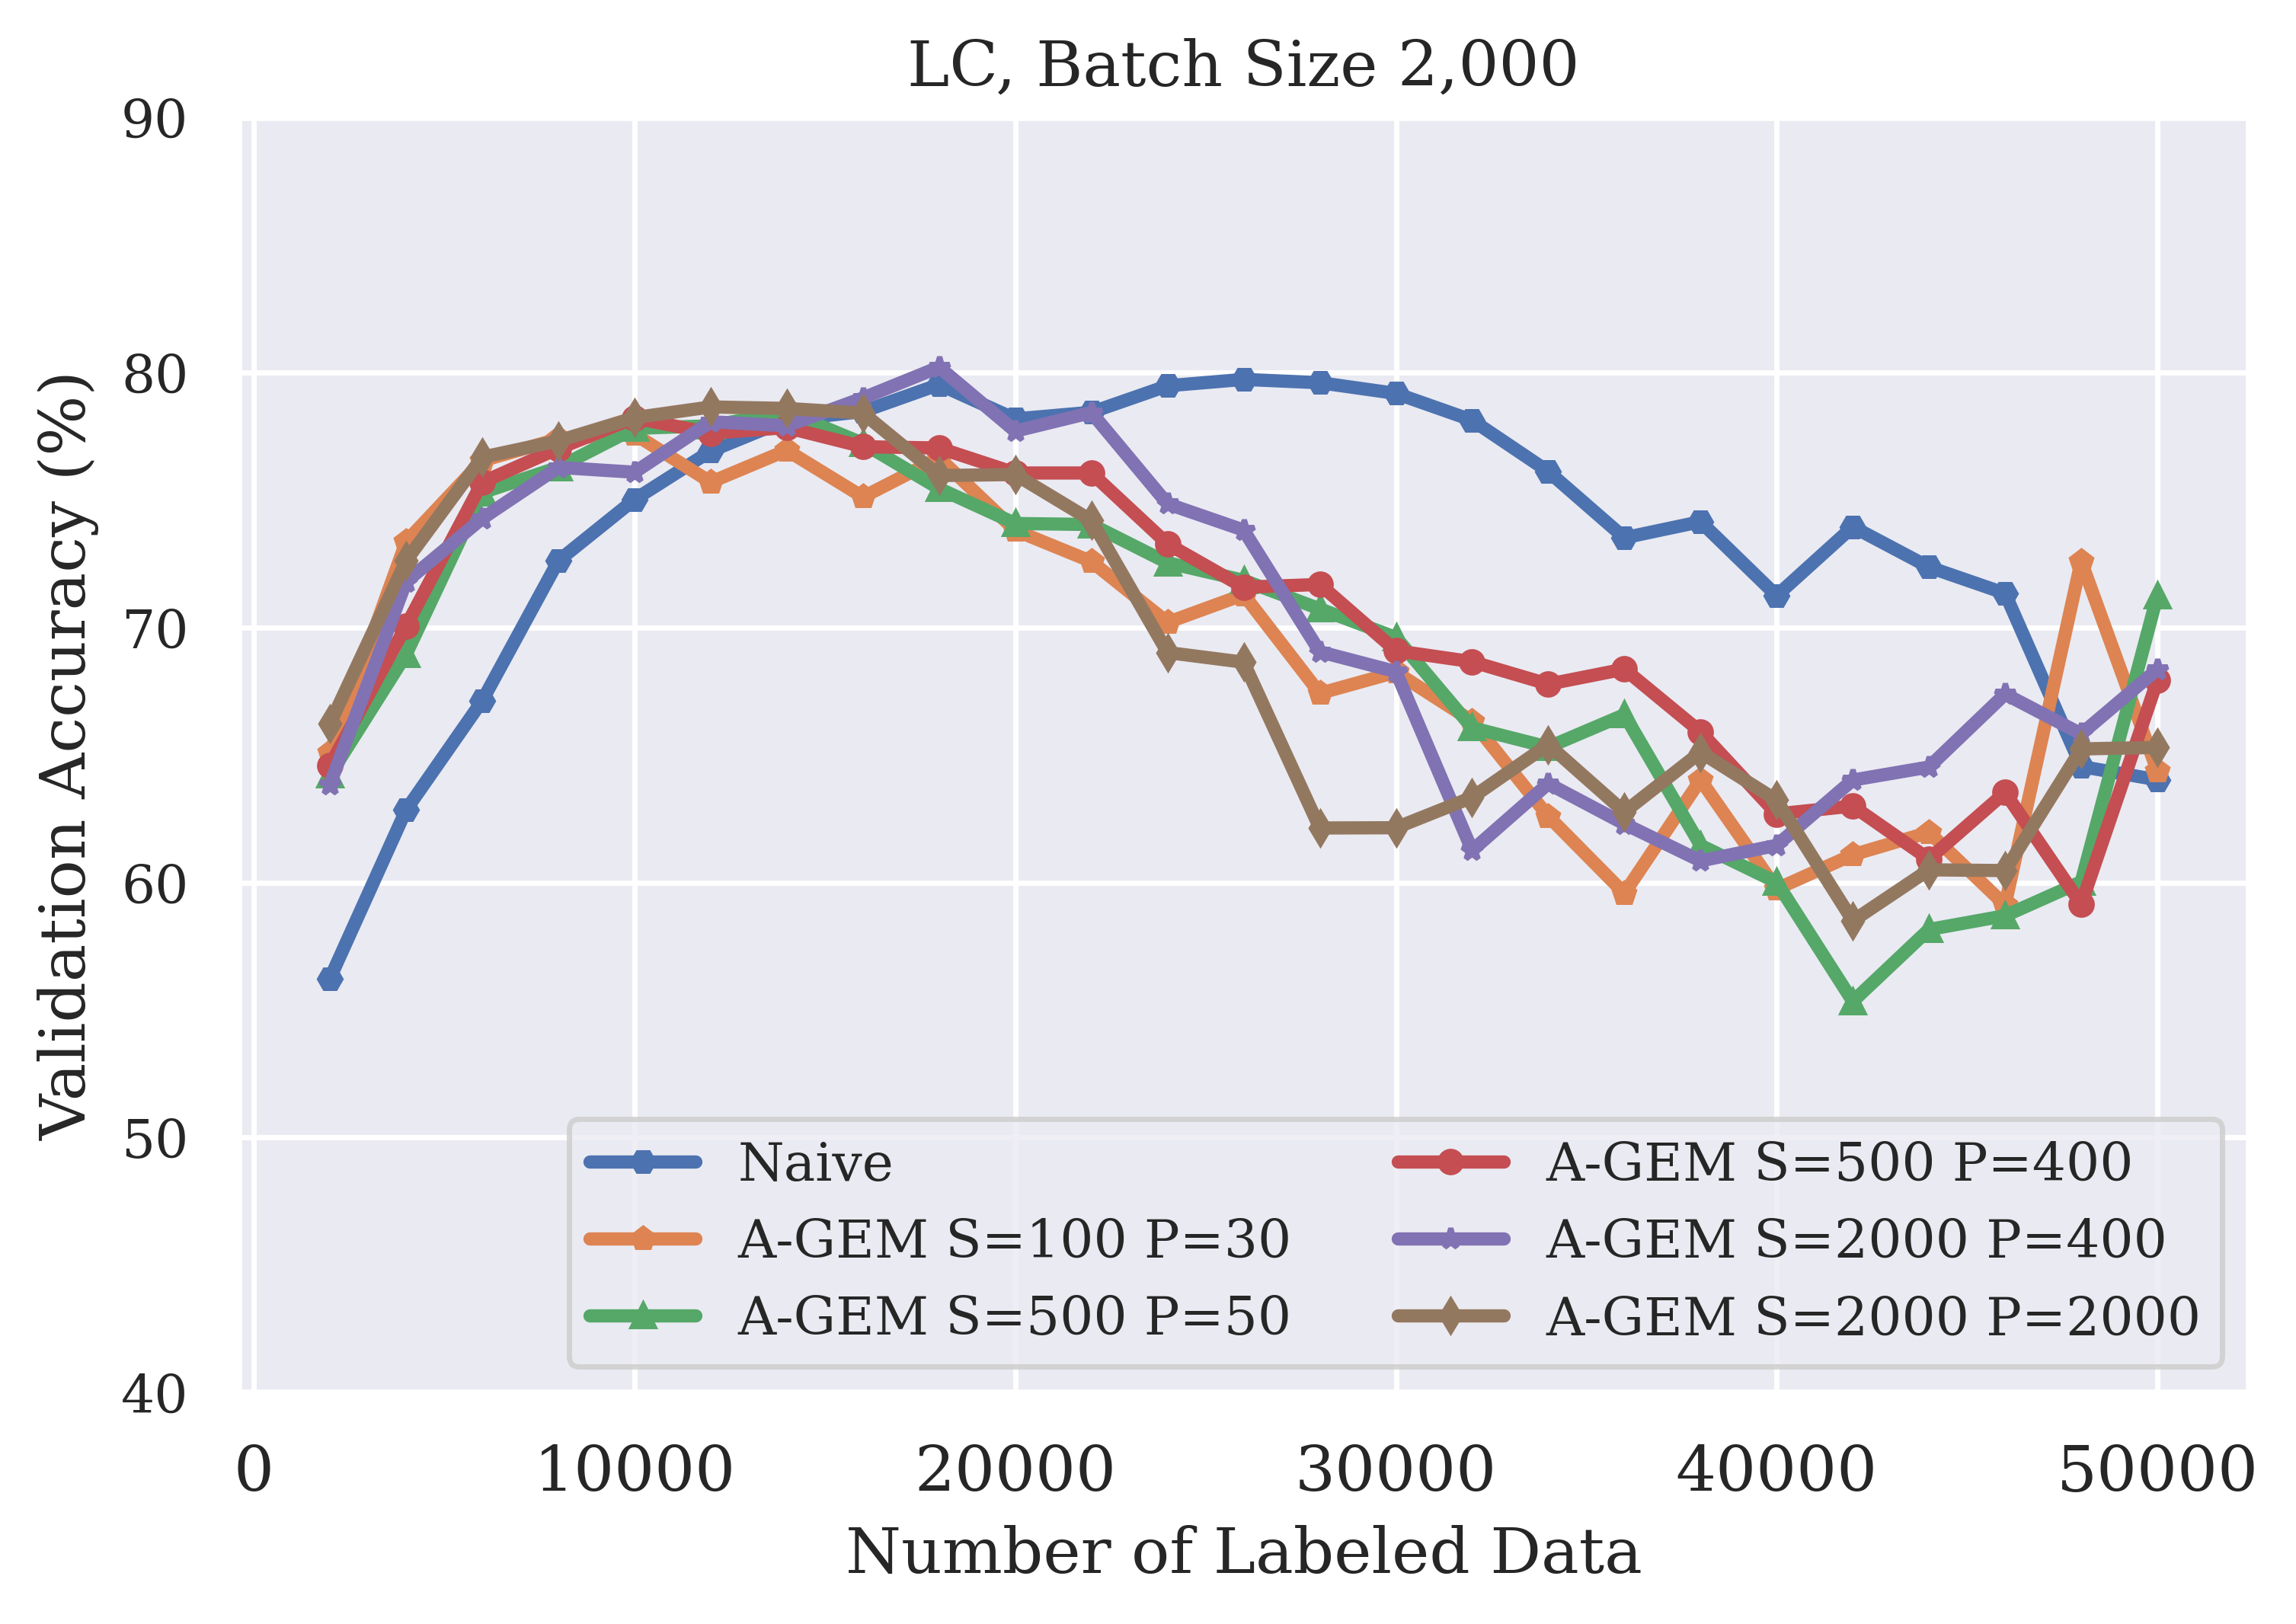
\includegraphics[width=0.48\linewidth]{images/results_CAL/agem_lc.png}
    \caption[Continual Active Learning with \gls{a-gem}]{Left: Comparison of validation accuracy of \gls{a-gem} to Naive with \gls{vaal} as the active learning strategy.
    Right: Validation accuracy of \gls{a-gem} for different values of $S$ and $P$.}
    \label{fig:Evaluation:Results:CAL:AGEM}
\end{figure}

In table \ref{fig:Evaluation:CAL:VAAL_AGEM_Time} we present the execution time of \gls{vaal} with active learning (baseline), \gls{vaal} and Naive as well as \gls{vaal}
and \gls{a-gem}. We notice that \gls{vaal} with \gls{a-gem} is significantly slower than the naive approach because of the costly computation of the reference
gradients. Overall, \gls{vaal} is among the slower active learning strategies due to the extensive training of the \gls{vae} and the discriminator on the
entire dataset. \par

\begin{table}[h]
    \centering
    \begin{tabular}{c | c } 
         & Execution time\\ 
        \hline 
        Baseline & 961 \\
        Naive & 341 \\
        \gls{a-gem} & 862 \\
    \end{tabular}
    \caption{Comparison of execution time using \gls{vaal}}
    \label{fig:Evaluation:CAL:VAAL_AGEM_Time}
\end{table}


\section{Continual Active Learning for Model Stealing}
\label{sec:Evaluation:MS}
After extensively studying continual active learning, we shift the focus of our experiments to model stealing. Since we build our work on the ActiveThief framework,
we first evaluate the performance of the ActiveThief framework, including the influence of model architecture and thief dataset. For these experiments, we refer to
section \ref{sec:Appendix:MS:ActiveThief} of the appendix. After experimenting with the ActiveThief framework, we evaluate the performance of continual active learning
for model stealing attacks. We perform experiments on the datasets MNIST, CIFAR-10, and CIFAR-100. Initially, we planned to compute the same experiments using ImageNet
as our target model dataset. We decided against running the experiments because our thief dataset is a subset of ImageNet, an unrealistic setting in 
the real world. Furthermore, the validation accuracy of the target model would most likely be lower than for CIFAR-100, making it even more challenging to
evaluate the different Continual Active Learning strategies because their performance would not differ significantly. First, we analyze continual active
learning using regularization-based continual learning strategies. Next, we move on to evaluate the combination of exemplar rehearsal continual learning and
representation-based active learning. \par


\subsection{Regularization-based Continual Learning}
\label{sec:Evaluation:MS:Regularization}

In this section, we evaluate the success of model stealing attacks using continual active learning with regularization-based continual learning strategies. 
We perform two sets of experiments: in the first set, the target model returns the predicted class label, and in the second set, the target model returns the
softmax probabilities for each class. The remaining setting for both sets of experiments is as follows: We use the target model datasets MNIST, CIFAR-10, and CIFAR-100,
the active learning strategies Random, \gls{lc}, \gls{bald}, \gls{badge} and CoreSet and the continual learning approaches Naive, \gls{ewc}, \gls{imm}, \gls{mas} and
\gls{alasso}. We use the ActiveThiefConv3 model as the target and substitute model and perform one model stealing attack for each combination of active learning,
continual learning strategy, and target model output. For the baseline runs, we use a batch size of 1,000 with a total query budget of 20,000. The query budget remains identical
for the continual active learning runs, but we increase the batch size to 2,000. \par
The numbers reported in the tables represent the model agreement at the end of each experiment, i.e., after using up the query budget of 20,000. Readers interested
in the progression of the model agreement across the experiments can find the respective plots in appendix \ref{sec:Appendix:CALMS}. As a baseline, we extract the models
using active learning with the strategies mentioned before. To evaluate the active learning strategies and the continual learning strategies, we compute the average
over the model agreement of all continual learning strategies combined with a fixed active learning strategy and the average of all active learning strategies combined
with a fixed continual learning strategy. These numbers are given at the end of each column and row, respectively. The active learning strategy and the continual
learning strategy with the highest average model agreement are highlighted in bold. \par


\subsubsection{Training with Predicted Labels}
\label{sec:Evaluation:MS:Regularization:Predicted}

In the first set of experiments, we perform model stealing attacks using the predicted class labels of the target model. We start with the target model dataset MNIST. 
The results of the experiments with MNIST are shown in table \ref{fig:ModelStealingMNISTLabel}. First, we observe a large margin between the model agreement
of the active learning strategies and the continual active learning strategies. However, the combination of \gls{bald} and Naive comes close to
its baseline. It demonstrates a model agreement of 69.18\%, about seven percentage points lower than the respective baseline. Overall, the naive approach performs
best with an average model agreement of 51.29\% across all active learning strategies. \gls{mas}, \gls{ewc} and \gls{imm} follow in that order, whereas \gls{alasso} 
suffers from exploding gradient problems and performs worst. The best active learning strategy is \gls{bald} with an average model agreement of 55.73\%. \gls{bald}
performs well in this setting because the substitute model, ActiveThiefConv3, contains dropout layers, which allow using Monte Carlo dropout for an accurate estimation
of $\mathbb{E}_{\theta \sim p(\theta \mid L)} [H[y \mid x, \theta]]$. \par

\begin{table}[h]
    \centering
    \begin{tabular}{c | c c c c c | c } 
         & Random & \gls{lc} & \gls{bald} & CoreSet & \gls{badge} & $\varnothing$ \\ 
        \hline
        Baseline & 67.56 & 80.36 & 76.29 & 81.62 & 76.43 & 76.45\\
        \hline
        Naive & 43.44 & 58.84 & 69.18 & 44.88 & 40.12 & \textbf{51.29}\\
        \gls{ewc} &  46.76 & 47.3 & 52.36 & 36.84 & 44.73 & 45.6\\
        \gls{imm} & 47.07 & 10.43 & 58.71 & 51.0 & 47.0 & 42.84\\
        \gls{mas} & 50.52 & 46.79 & 49.51 & 44.96 & 49.47 & 48.25\\
        \gls{alasso} & 10.44 & 46.89 & 48.89 & 16.27 & 10.43 & 26.68\\
        \hline
        $\varnothing$ & 39.65 & 50.97 & \textbf{55.73} & 38.79 & 38.35 & -\\
    \end{tabular}
    \caption{Model agreement of continual learning strategies on MNIST using the predicted class label}
    \label{fig:ModelStealingMNISTLabel}
\end{table}


For the next set of experiments, we use the target model dataset CIFAR-10 and present our results in table \ref{fig:ModelStealingCIFAR10Label}. 
Across the board, the model agreement is lower than in the previous experiment because the CIFAR-10 dataset is more complex than MNIST. Interestingly, the ranking of
the continual learning strategies has changed significantly. \gls{ewc} is now the best performing strategy, followed by \gls{imm} and Naive. \gls{mas} and \gls{alasso}
perform worst. The main reason for the large gap between the naive approach and \gls{ewc} as well as \gls{imm} is the poor performance of \gls{bald} and Naive.
Surprised by the poor performance of this combination, we re-run the experiment and received similar results. We assume that the poor model agreement, initially
caused by the complexity of the dataset, makes it difficult for \gls{bald} to find informative samples. The best active learning strategy is CoreSet, with an average
model agreement of 43.57\%. Random follows next, outperforming \gls{badge}, \gls{lc}, and \gls{bald}. \par

\begin{table}[h]
    \centering
    \begin{tabular}{ c | c c c c c | c } 
         & Random & \gls{lc} & \gls{bald} & CoreSet & \gls{badge} & $\varnothing$\\ 
        \hline
        Baseline & 60.23 & 49.73 & 61.28 & 63.78 & 62.26 & 59.46\\
        \hline
        Naive & 49.84 & 30.03 & 10.18 & 48.44 & 45.25 & 36.75\\
        \gls{ewc} & 50.37 & 47.12 & 50.22 & 47.94 & 49.11 & \textbf{48.95} \\
        \gls{imm} & 49.84 & 44.25 & 43.55 & 49.64 & 48.22 & 47.1\\
        \gls{mas} & 45.76 & 33.27 & 36.87 & 39.98 & 40.24 & 32.02\\
        \gls{alasso} & 19.05 & 38.16 & 30.91 & 31.86 & 25.04 & 29.0\\
        \hline
        $\varnothing$ & 42.97 & 38.57 & 34.35 & \textbf{43.57} & 41.57 & -\\
    \end{tabular}
    \caption{Model agreement of continual learning strategies on CIFAR-10 using the predicted class label}
    \label{fig:ModelStealingCIFAR10Label}
\end{table}


Finally, we compute the model agreement using CIFAR-100 as our target model dataset. When starting experiments with \gls{badge}, we observed that they
took significantly longer than the other experiments. We investigated this further and found the estimated runtime to be more than 40 days using our hardware
This is why we could not deliver results for this combination.  \gls{badge} has a high runtime because its query time scales linearly with the number of classes. Since
CIFAR-100 has 100 classes, the query time is ten times longer than the query time on CIFAR-10, which took four days. We present our results in table 
\ref{fig:ModelStealingCIFAR100Label}. Across the board, the model agreement has decreased compared to the previous experiment, which is again due to increased dataset
complexity. While the absolute gap between the continual learning methods and the baseline is smaller than in the previous experiments, the relative gap has increased
significantly. The baseline strategies boast a model agreement of 20.42\% on average, whereas the best continual learning strategy, which is \gls{imm}, demonstrates a
model agreement of 8.07\% on average. \gls{imm} significantly outperforms both the naive approach and \gls{ewc}, which exhibit almost identical performance. We were surprised
by the poor performance of \gls{ewc} and \gls{bald}, which is why we conducted this experiment one more time, however, we achieved similar results. The remaining
continual learning strategies, \gls{mas} and \gls{alasso}, perform worse than the naive approach. Remarkably, \gls{alasso} outperforms \gls{mas}, making this the
only set of experiments in which \gls{alasso} is not the worst-performing continual learning strategy. Another surprise is the performance of the random sampling,
which outperforms the remaining active learning strategies. CoreSet, which demonstrated strong performance in previous experiments, falls behind
Random and \gls{lc}, outperforming only \gls{bald} by about one percentage point. CoreSet fails to perform in this setting because the uncertainty of its query
selection increases with the number of classes \cite{sener2017active}. \par

\begin{table}[h]
    \centering
    \begin{tabular}{ c | c c c c | c } 
         & Random & \gls{lc} & \gls{bald} & CoreSet & $\varnothing$\\ 
        \hline
        Baseline & 21.65 & 19.5 & 19.64 & 20.9 & 20.42\\
        \hline
        Naive & 7.93 & 7.63 & 4.98 & 4.82 & 6.34\\
        \gls{ewc} & 8.79 & 6.55 & 2.07 & 7.77 & 6.3\\
        \gls{imm} & 8.59 & 8.44 & 7.18 & 8.05 & \textbf{8.07}\\
        \gls{mas} & 5.37 & 5.44 & 5.3 & 4.52 & 5.16\\
        \gls{alasso} & 5.28 & 6.11 & 5.72 & 5.51 & 5.66\\
        \hline
        $\varnothing$ & \textbf{7.19} & 6.83 & 5.05 & 6.13 & -\\
    \end{tabular}
    \caption{Model agreement of continual learning strategies on CIFAR-100 using the predicted class label}
    \label{fig:ModelStealingCIFAR100Label}
\end{table}




\subsubsection{Training with Softmax Probabilities}
\label{sec:Evaluation:MS:Regularization:Softmax}

We move on to the second set of experiments, in which we train the substitute model using the softmax probabilities of the target model. First, we compute model agreement
on the MNIST dataset. The results of this experiment can be found in table \ref{fig:ModelStealingMNISTSoftmax}. In terms of the model agreement, all continual
active learning attacks perform significantly worse than the baseline. The best-performing attack \gls{bald} with \gls{mas}, achieving a model
agreement of 67.84\%. The most performant active learning strategy is \gls{bald} with an average model agreement of 52.52\%, whereas the best continual learning strategy is
\gls{mas}. \gls{mas} achieves an average model agreement of 57.73\%. While the continual learning strategies struggled to outperform the naive approach in previous experiments,
most of them outperform the naive approach in the Model Stealing setting. The only exception to this is \gls{alasso} which experiences exploding gradient problems. Overall,
the model agreement is about ten percentage points higher than training with the predicted label. This is because the softmax probabilities reveal more about the target model's
learned prediction function than the predicted label. \par 

\begin{table}[h]
    \centering
    \begin{tabular}{ c | c c c c c | c } 
         & Random & \gls{lc} & \gls{bald} & CoreSet & \gls{badge} & $\varnothing$\\ 
        \hline
        Baseline & 87.91 & 82.39 & 83.64 & 91.22 & 79.68 & 84.97\\
        \hline
        Naive & 47.74 & 43.02 & 59.61 & 58.36 & 48.89 & 51.52\\
        \gls{ewc} &  59.26 & 53.67 & 59.18 & 56.13 & 50.28 & 55.7\\
        \gls{imm} & 48.18 & 62.95 & 49.71 & 63.43 & 58.76 & 56.61 \\
        \gls{mas} &  64.42 & 50.27 & 67.84 & 55.58 & 50.54 & \textbf{57.73}\\
        \gls{alasso} & 28.04 & 15.5 & 26.28 & 10.39 & 12.8 & 20.6\\
        \hline
        $\varnothing$ & 49.57 & 45.08 & \textbf{52.52} & 48.78 & 44.24 & -\\
    \end{tabular}
    \caption{Model agreement of continual learning strategies on MNIST using softmax output}
    \label{fig:ModelStealingMNISTSoftmax}
\end{table}


We move on to the dataset CIFAR-10. Our results are shown in table \ref{fig:ModelStealingCIFAR10Softmax}. Similar to our findings from previous experiments, the baseline outperforms 
the continual active learning approaches. However, the difference in performance between them is marginal at a maximum of 12 percentage points.
\gls{alasso} is an exception to this, performing significantly worse than the other continual learning strategies due to exploding gradient problems. The best continual active
learning strategy is \gls{ewc} with an average model agreement of 60.14\%. At the same time, \gls{ewc} is the only continual learning strategy to outperform the naive approach,
albeit the margin between the two is only 0.48 percentage points. Overall, CoreSet is the most performant active learning strategy, achieving an average model agreement of 54.12\%. \par

\begin{table}[h]
    \centering
    \begin{tabular}{ c | c c c c c | c } 
         & Random & \gls{lc} & \gls{bald} & CoreSet & \gls{badge} & $\varnothing$\\ 
        \hline 
        Baseline & 71.58 & 70.04 & 71.96 & 71.45 & 71.44 & 71.29\\
        \hline
        Naive & 60.8 & 56.62 & 61.84 & 61.61 & 57.42 & 59.66 \\
        \gls{ewc} & 58.67 & 56.8 & 61.57 & 61.79 & 61.88 & \textbf{60.14}\\
        \gls{imm} & 60.78 & 52.24 & 60.32 & 61.39 & 56.98 & 58.34 \\
        \gls{mas} & 50.32 & 51.45 & 52.09 & 52.23 & 55.68 & 52.35\\
        \gls{alasso} & 17.26 & 24.87 & 28.24 & 33.59 & 32.93 & 27.38\\
        \hline
        $\varnothing$ & 49.57 & 48.4 & 52.81 & \textbf{54.12} & 52.98 & -\\
    \end{tabular}
    \caption{Model agreement of Continual Learning strategies on CIFAR-10 using softmax output}
    \label{fig:ModelStealingCIFAR10Softmax}
\end{table}


Finally, we experiment with the CIFAR-100 dataset. As in section \ref{sec:Evaluation:MS:Regularization:Predicted}, we omit the results for \gls{badge} due to their high runtime.
The results for the remaining combinations can be found in table \ref{fig:ModelStealingCIFAR100Softmax}. Across the board, the model agreement is
significantly lower than for MNIST and CIFAR-10, caused by the complexity of this dataset. In this setting,
\gls{ewc} outperforms the remaining continual learning strategies, and it is one of two continual learning strategies, which outperform the naive approach.
The other strategy is \gls{imm}, which puts on a performance in between \gls{ewc} and the naive approach. \gls{mas} follows behind the naive approach
and \gls{alasso} is left behind. The best active learning strategy is CoreSet, which outperforms \gls{bald} by 0.57 percentage points.\par

\begin{table}[h]
    \centering
    \begin{tabular}{ c | c c c c | c } 
         & Random & \gls{lc} & \gls{bald} & CoreSet & $\varnothing$\\ 
        \hline
        Baseline & 25.43 & 26.92 & 28.01 & 27.48 & 26.96 \\
        \hline
        Naive & 18.46 & 18.48 & 16.8 & 17.69 & 17.86\\
        \gls{ewc} & 19.45 & 17.46 & 20.67 & 19.98 & \textbf{19.39}\\
        \gls{imm} & 18.16 & 17.9 & 20.39 & 18.75 & 18.8\\
        \gls{mas} & 15.75 & 14.85 & 14.72 & 15.45 & 15.19\\
        \gls{alasso} & 5.2 & 4.95 & 6.7 & 10.24 & 6.77\\
        \hline
        $\varnothing$ & 15.4 & 14.73 & 15.85 & \textbf{16.42} & -\\
    \end{tabular}
    \caption{Model agreement of continual learning strategies on CIFAR-100 using softmax output}
    \label{fig:ModelStealingCIFAR100Softmax}
\end{table}



\subsection{Exemplar Rehearsal Continual Learning and Representation-based Active Learning}
\label{sec:Evaluation:CALMS:VAAL_AGEM}

After conducting our experiments with regularization-based continual learning strategies, we test the combination of the active learning strategy \gls{vaal}
with the continual learning strategy \gls{a-gem}. We motivate this experiment by the performance of \gls{vaal} and \gls{a-gem} in the classic continual
learning setup, given in figure \ref{fig:Evaluation:Results:CAL:AGEM}. We conduct the experiments with the same hyperparameters as in section 
\ref{sec:Evaluation:MS:Regularization}. To evaluate the performance of \gls{vaal} and \gls{a-gem}, we compare the results to the best performing active
learning strategy from the experiments in section \ref{sec:Evaluation:MS:Regularization}, CoreSet, and the combination of the best
performing continual learning strategy and the most performant active learning strategy, which are \gls{ewc} and CoreSet, respectively. The results are given
in Table \ref{fig:ModelStealingVAALAGEM}. We present the model agreement progression with \gls{vaal} and \gls{a-gem} in appendix
\ref{sec:Appendix:CALMS:VAALAGEM}. While \gls{vaal} and \gls{a-gem} cannot keep up with the performance of the baseline, it outperforms CoreSet and \gls{ewc}
in three out of six experiments while being outperformed in the remaining three. \par

\begin{table}[h]
    \centering
    \begin{tabular}{c | c  c  | c  c | c  c } 
        \multirow{2}*{Attack strategy}& \multicolumn{2}{c |}{MNIST} & \multicolumn{2}{c |}{CIFAR-10} & \multicolumn{2}{c}{CIFAR-100}  \\ 
         & Softmax & Label & Softmax & Label & Softmax & Label \\
        \hline 
        \gls{vaal} \gls{a-gem} & 52.54 & 53.8 & 61.48 & 50.5 & 18.29 & 8.77\\
        CoreSet \gls{ewc} & 56.13 & 36.84 & 61.79 & 47.94 & 19.98 & 7.77 \\
        Coreset Baseline & 90.65 & 77.58 & 71.61 & 61.68 & 27.52 & 20.96\\
    \end{tabular}
    \caption{Comparison of model agreement using \gls{vaal} and \gls{a-gem}}
    \label{fig:ModelStealingVAALAGEM}
\end{table}
